\documentclass[12pt, letter]{article}	
\renewcommand*\rmdefault{bch}
\usepackage{amssymb}
\usepackage[utf8]{inputenc}
\usepackage[ignorehead]{geometry}
\usepackage{amsmath}
\usepackage{bbm}
\usepackage{amsfonts}
\usepackage{graphicx}
\usepackage[doublespacing]{setspace}
\usepackage{appendix}
\usepackage{fancybox}
\usepackage{ltxtable}
\usepackage{acronym}
\usepackage{eurosym}
\usepackage{textcomp}
\usepackage{appendix}
\usepackage[justification=justified]{caption}
\usepackage[dvipsnames,table]{xcolor}
\usepackage[final]{pdfpages}
\usepackage{eso-pic}
\usepackage{everyshi}
\usepackage{booktabs}
\usepackage{fancyhdr}
\usepackage{tabu}
\usepackage{threeparttable}
\usepackage{bbm}
\usepackage{amssymb}
\usepackage{multirow}
\usepackage{indentfirst}
\usepackage{float}
\usepackage{placeins}
\usepackage{natbib}
\usepackage{mdframed}
\usepackage{rotating}
\usepackage{tabularx}
\usepackage{comment}
%\usepackage[maxbibnames=99]{biblatex}
%\bibliographystyle{elsarticle-harv}
%\usepackage{hyperref}
\usepackage[colorlinks=true,citecolor=Blue,linkcolor=black,urlcolor=teal,linktoc=all]{hyperref} %Allows links to URLs
	\definecolor{darkblue}{rgb}{0.0,0.0,0.3}
	\hypersetup{urlcolor=darkblue}
\setcounter{MaxMatrixCols}{30}
\usepackage{subfig}
\usepackage{tikz}
\usetikzlibrary{decorations.pathreplacing}

\usepackage[stable]{footmisc}


\usepackage{epigraph}
\usepackage{lscape} % Makes a single page landscape

\setlength\epigraphwidth{16cm}
\setlength\epigraphrule{0pt}

% change the url font to the normal font
\usepackage{url} \urlstyle{same}
% force url to break like normal text (not just at slash)
\expandafter\def\expandafter\UrlBreaks\expandafter{\UrlBreaks%  save the current one
  \do\a\do\b\do\c\do\d\do\e\do\f\do\g\do\h\do\i\do\j%
  \do\k\do\l\do\m\do\n\do\o\do\p\do\q\do\r\do\s\do\t%
  \do\u\do\v\do\w\do\x\do\y\do\z\do\A\do\B\do\C\do\D%
  \do\E\do\F\do\G\do\H\do\I\do\J\do\K\do\L\do\M\do\N%
  \do\O\do\P\do\Q\do\R\do\S\do\T\do\U\do\V\do\W\do\X%
  \do\Y\do\Z}

\usepackage{array}
\usepackage{tabularx}
				\newcolumntype{C}{>	{\centering\arraybackslash}X}% Horizonal center, vertical center
				\newcolumntype{L}{>	{\raggedright\arraybackslash}X}% Horizonal left, vertical center
				\newcolumntype{R}{>	{\raggedleft\arraybackslash}X}% Horizonal right, vertical center
				\newcolumntype{T}{>	{\hsize=.25\hsize}X}% raggedleft column X

\providecommand{\U}[1]{\protect\rule{.1in}{.1in}}

\newtheorem{theorem}{Theorem}
\newtheorem{acknowledgement}{Acknowledgement}
\newtheorem{algorithm}{Algorithm}
\newtheorem{assumption}{Assumption}
\newtheorem{axiom}{Axiom}
\newtheorem{case}{Case}
\newtheorem{claim}{Claim}
\newtheorem{conclusion}{Conclusion}
\newtheorem{condition}{Condition}
\newtheorem{conjecture}{Conjecture}
\newtheorem{corollary}{Corollary}
\newtheorem{criterion}{Criterion}
\newtheorem{definition}{Definition}
\newtheorem{example}{Example}
\newtheorem{exercise}{Exercise}
\newtheorem{lemma}{Lemma}
\newtheorem{notation}{Notation}
\newtheorem{problem}{Problem}
\newtheorem{proposition}{Proposition}
\newtheorem{remark}{Remark}
\newtheorem{solution}{Solution}
\newtheorem{summary}{Summary}
\newenvironment{proof}[1][Proof]{\noindent\textbf{#1.} }{\ \rule{0.5em}{0.5em}}
\geometry{margin=1in,top=1in,bottom=1in}
\renewcommand{\thesection}{\arabic{section}}
\renewcommand{\thesubsection}{\arabic{section}.\arabic{subsection}}
\renewcommand{\thesubsubsection}{\arabic{section}.\arabic{subsection}.\arabic{subsubsection}}
%\renewcommand{\thefootnote}{\fnsymbol{footnote}}
\onehalfspacing
\makeatletter
\def\@biblabel#1{\hspace*{-\labelsep}}
\def\hyph{-\penalty0\hskip0pt\relax}
\makeatother
%\pagenumbering{roman}
\renewcommand*\thetable{\arabic{table}}
\renewcommand*\thefigure{\arabic{figure}}
\mathchardef\mhyphen="2D

\interfootnotelinepenalty=10000


%Displaystyle
	\newcommand{\ds}{\displaystyle}
	\DeclareMathOperator*{\mean}{mean}




\begin{document}

%\title{Learning by Doing and Technological Path: Industrial Policies in the Chinese Solar Panel Industry}
\title{Learning-by-Doing and Industrial Policies: Evidence from China's Solar Panel Industry}
\author{Dana Golden \and Xiangjun Ma \and  Yiyi Zhou\thanks{Golden: Department of Economics, Stony Brook University, dana.golden@stonybrook.edu. Ma: School of Finance and Trade, Liaoning University, aqj474@gmail.com. Zhou: Department of Economics, Stony Brook University, yiyi.zhou@stonybrook.edu.}}

\maketitle

\begin{abstract}

\singlespacing 

Crystalline silicon (c-Si) technology has dominated in the solar panel manufacturing and the production costs have declined by \textcolor{blue}{XX\%} over the past decade. This study investigates the role of learning-by-doing (LBD) in driving this cost reduction and forming the technological pathway of the industry, and its interaction with input price and government subsidy policies.



\thispagestyle{empty}

\begin{description}
\item[Keywords:] 

\item[JEL Classification Codes:] 
\end{description}
\end{abstract}

%\newpage\tableofcontents

\clearpage
\setcounter{page}{1}

\section{Introduction}

The development of solar energy plays a crucial role in the transition to a sustainable and low-carbon electricity grid and the mitigation of climate change. In recent decades, production costs of solar panel have fallen by \textcolor{blue}{XX\%}. Meanwhile, the share of solar panel manufactured using crystalline silicon (c-Si) technology has increased from \textcolor{red}{90\% ?} in 2000 to 98\% in 2020. Industry experts have attributed this technological dominance and this substantial cost reduction largely to learning-by-doing (LBD), the maturing of upstream industries, and industrial policies. Nonetheless, during this period of time, polysilicon, the main input of c-Si technology, experienced a price reduction of 95\% between 2008 and 2013 while the prices of the main input of competing thin-film technology have remained relatively stable.

While industrial policies are often controversial in many sectors, certain important features of renewable energy, such as solar panel in this study, deserve careful consideration. Subsidies on either demand or supply side can be justified due to various market failures, including environmental externalities and knowledge spillovers. In addition, individual countries may benefit from government support or protection when the industry is still in its infancy.
However, how LBD interacts with industrial policies to shape production costs and technological pathways is not well understood. This paper aims to fill this gap by quantifying the extent to which LBD contributes to reducing solar panel cost and driving the growth of the c-Si technology, and by evaluating how industrial policies on both demand and production sides influence solar panel diffusion, the expansion of the c-Si technology, and overall social welfare.

Quantifying LBD is crucial for evaluating the impacts of various industrial policies. 
Subsidies aimed at promoting solar panel adoption have been widely implemented by governments worldwide. LBD creates a positive ``feedback loop", analogous to the mechanism described in \citet{barwick2025drive} on the interaction between the EV subsidies and the LBD in battery manufacturing. In our setting, demand-side subsidies stimulate greater solar panel uptake, which increases manufacturers’ production experience. This accumulated experience strengthens LBD, driving down production costs and solar panel prices, which in turn further increases adoption and magnifies the overall impact of demand-side subsidies.

Industrial policies aimed at fostering the development of upstream industries have been adopted by most governments in recent years. China, for example, supported the establishment of a domestic silicon sector, although initially to provide inputs for semiconductors rather than solar panel. This support was proved to be advantageous when silicon prices spiked in late 2007, which was also the first year the solar industry used more silicon worldwide than the chip industry. More recently, the U.S. has offered generous support to the manufacture of rare earth elements which are key inputs of semiconductors. 
LBD also generates a positive ``feedback loop": falling prices of a key input of a particular technology induce firms to adopt that technology, which increases experience in production of that cheaper-input technology. LBD associated with the enhanced production experience of the cheaper-input technology further reduces the cost of the cheaper-input technology and solar panel price. These cost and price reductions of the cheaper-input technology, in turn, further accelerate the adoption of that technology, amplifying the direct effects of demand- and supply-side policies.
%\textcolor{blue}{But this is more a concern for national security than bringing down the input price??} 
% This support was proved to be advantageous when silicon prices spiked in late 2007, which was also the first year the solar industry used more silicon worldwide than the chip industry. 
%Other examples include semiconductors that are highly dependent on the supply and cost of highly purified silicon and rare earth elements, and electric vehicles that are highly dependent on the efficiency of battery production. 
% In recent years, many governments give preferential treatment of domestic input producers. Taking electric vehicle as an example. China implemented a whitelist policy that restricted EV subsidies to vehicles using batteries from government-approved domestic producers. The U.S. IRA mandates EV models to source a certain fraction of critical minerals and battery components from firms in North American or free-trade agreement partner countries. 

\textcolor{blue}{[Describe our model!]}

Our empirical analysis delivers three key findings. First, the learning rate is estimated to be \textcolor{blue}{XX\%} after controlling for .... That is, doubling solar panel manufactures' production experience would reduce unit production costs by \textcolor{blue}{XX\%}. This implies that LBD alone accounted for \textcolor{blue}{XX\%} of the overall decline in the solar panel costs from 2000 to 2013. \textcolor{blue}{Compare with other studies on learning rates. For example, \citet{barwick2025drive} finds a learning rate of 7.5\% of EV battery production from 2013 to 2020.}

Second, LBD greatly amplifies the impact of the price decline of silicon through positive feedback loops. In the absence of LBD, the price drop of silicon is estimated to increase cumulative solar panel sales by \textcolor{blue}{XX\%} and increase the share of c-Si technology by \textcolor{blue}{XX\%} during the sample period. When LBD was also in effect, solar panel sales surged by \textcolor{blue}{XX\%} and the share of s-Si technology increased by \textcolor{blue}{XX\%} relative to the baseline with neither silicon price drop nor LBD. This combined effect is \textcolor{blue}{XX\%} greater than the sum of the effects from silicon price drop and LBD individually, suggesting their complementarity. 


Third, LBD greatly amplifies the impact of subsidies, including subsidies on installation and subsidies on production costs and entry costs. In the absence of LBD, subsidies across different regions are estimated to increase cumulative solar panel sales by \textcolor{blue}{XX\%} during the sample period. When both subsidies and LBD were in effect, solar panel sales surged by \textcolor{blue}{XX\%} relative to the baseline with neither subsidies nor LBD.  These findings highlight the importance of accounting for LBD when evaluating the efficacy and cost-effectiveness of government policies designed to promote solar panel production and adoption. Ignoring LBD would lead to a substantial underestimation of the long-term benefits of such policies.



\subsection*{Literature}

\paragraph{Industrial Policies of solar panel}
%Our paper contributes to the large literature on industrial policy in general. Most previous studies examine the pros and cons of an industrial policies and which industries should be targeted. For example, XXX analyzes trade policies, XXX studies R\&D subsidies, and XX examine environmental subsidies. Exceptions include \citet{barwick2025industrial} on the Chinese shipbuilding industry, \citet{bai2020quid} on the Chinese Auto industry, \citet{barwick2024attribute} on electric vehicles, and \citet{barwick2025drive} on the global EV battery industry. 

Our paper contributes to the growing literature that studies policies in the solar panel industry. Many of these studies, including \citet{de2019subsidies}, focus on the impact of demand-side subsidies. One exception is
\citet{bollinger2025strategic}, who examines how import tariffs affect market equilibrium outcomes and compares import tariffs to supply-side subsidies. 
To the best of our knowledge, our study is the first to study the impact of both demand- and supply-side policies on the production cost and technological pathways, explicitly accounting for LBD. Our results highlight that ignoring LBD would significantly underestimate the impact of government policies on solar panel adoption.


\paragraph{Learning by Doing}
Our paper contributes to the empirical literature on LBD that has been documented in a variety of industries, for example, \citet{head1994infant} and \citet{ohashi2005learning} on steel, \citet{thompson2001much} and \citet{thornton2001learning} on shipbuilding, \citet{benkard2000learning} and \citet{benkard2004dynamic} on aircraft, \citet{su2025LBD} on space launch and etc. Almost all previous studies relied on data on input requirements or costs associated with producing a product, but these data are often hard to obtain for researchers. Exceptions include \citet{covert2022winds} and \citet{barwick2025drive}. Our approach is in the same spirit of theirs by exploiting variations in prices and quantities of the final products (solar panel) and main inputs (polysilicon for c-Si technology and Cadmium and Tellurium for thin-film technology).

In particular, our paper contributes to the growing literature studying learning-by-doing in low-carbon technology sectors, such as solar panel, wind generating systems, and electric vehicles. 
\citet{barwick2025drive} ...
\citet{helveston2022quantifying} estimates a two-factor learning model using the annual installed capacities and prices of solar panel modules in Germany, U.S., and China between 2006 to 2020 and finds that the learning rates are 20\%, 26\%, and 33\% in these three countries, respectively.

\paragraph{Technological Path}


%\paragraph{Supply Chain}
%\citet{barwick2025drive} examines how the industrial policies of downstream (electric vehicles) market and the learning-by-doing of upstream (battery) production affect the production cost of upstream (battery). In contrast, our paper studies how the price decline of upstream product (silicon), and the learning-by-doing and industrial policies of downstream (solar panel) production affect the production cost and the technological pathways of downstream (solar panel).


\paragraph{Estimation of Dynamic Games}
Finally, our paper is build on the literature on the estimation of dynamic games, including \citet{bajari2007estimating}, \citet{ryan2012costs}, and \citet{sweeting2013dynamic}.

\section{Solar Panel Industry and Data}
\label{sec:institution_data}

\subsection{Technologies of Solar Panel Manufacturing}
\label{subsec:inst_PV_tech}

There have been two major technologies to manufacture solar panel in the past three decades.  The first one is the crystalline silicon technology (c-Si), which was invented by scientists at Bell labs in 1954. Crystalline silicon technology was initially utilized in space installations before being used in the first solar building at the University of Delaware in 1973. Silicon panels quickly improved from below 10\% efficiency at inception to 20\% efficiency in the field currently. Crystalline silicon benefits greatly from its durability and efficiency. A power plant developed using crystalline silicon will require a significantly smaller area than a power plant developed using thin-film technology. The technology was invented and first commercialized in the United States with the United States still the largest manufacturer through 2010 before becoming a technology dominated by China in the 2010s.

Most c-Si solar panels are  produced by vertically integrated manufacturers that use polysilicon to manufacture wafers, then process these wafers into solar cells that generate electricity through the photovoltaic effect, and finally assemble the cells into solar panels (or ``modules"). Because this technology is highly commoditized, we treat solar panels as homogeneous, conditional on the underlying production technology. This assumption is further supported by \citet{bollinger2025strategic} who analyze a dataset of solar panel shipments to the US, constructed from quarterly IHS Markit data, and find very little price dispersion across manufacturers at any given time. 

Crystalline silicon competes the thin-film technology, which can be made from a variety of materials including Cadmium, Tellurium, and Silver. Compared with c-Si technology, the thin-film technology is less efficient -- that is, it converts a smaller proportion of solar energy into electricity. However, the thin-film technology is more flexible and potentially can be used in a wider variety of configurations. The lower fixed costs and flexibility associated with thin-film technologies made them ideal for traveling outdoors and other adaptable situations. This made them more commonly used in countries like the United States and less commonly used for utility-scale power generation. Moreover, material costs are stable and projected to be cheaper. The major inputs such as Cadmium and Tellurium are the by products of steel production.

Figure \ref{fig:data_sum_two_tech_price_output} displays the price and installed capacity of the two types of solar panel since 2000. Over the last two decades, there has been a significant decrease in global solar panel prices, with the most noticeable decline occurring after 2008. This price decline has spurred the installation of solar panels worldwide. Additionally, the rapid expansion of solar panel installations is driven by government subsidies on a global scale. %A common policy involves providing tax rebates or credits that lower the out-of-pocket expenses for consumers. For instance, the United States initially offered a subsidy covering 30 percent of the system cost, which later increased to 40 percent by the end of the period.  Another prevalent policy is the implementation of feed-in tariffs designed to incentivize solar energy production. These feed-in tariffs can be substantial, reaching up to 50 percent in Japan in 2012. Meanwhile, governments may also impose tariffs on imported solar panel systems to safeguard domestic production, which raises consumer prices. In the past two decades, tariffs were increased due to dumping concerns, with the most significant hikes observed in the United States, reaching 35 percent, and in India, reaching 20 percent. \textcolor{blue}{Make sure the specific time periods of the tariffs.}


%    \begin{figure}
%     \caption{Price and Installed Capacity}
%     \label{fig:data_sum_two_tech_price_output}
%     \centering
%     %\hfill
%     \begin{subfigure}[t]{0.40\textwidth}
%         \centering
%         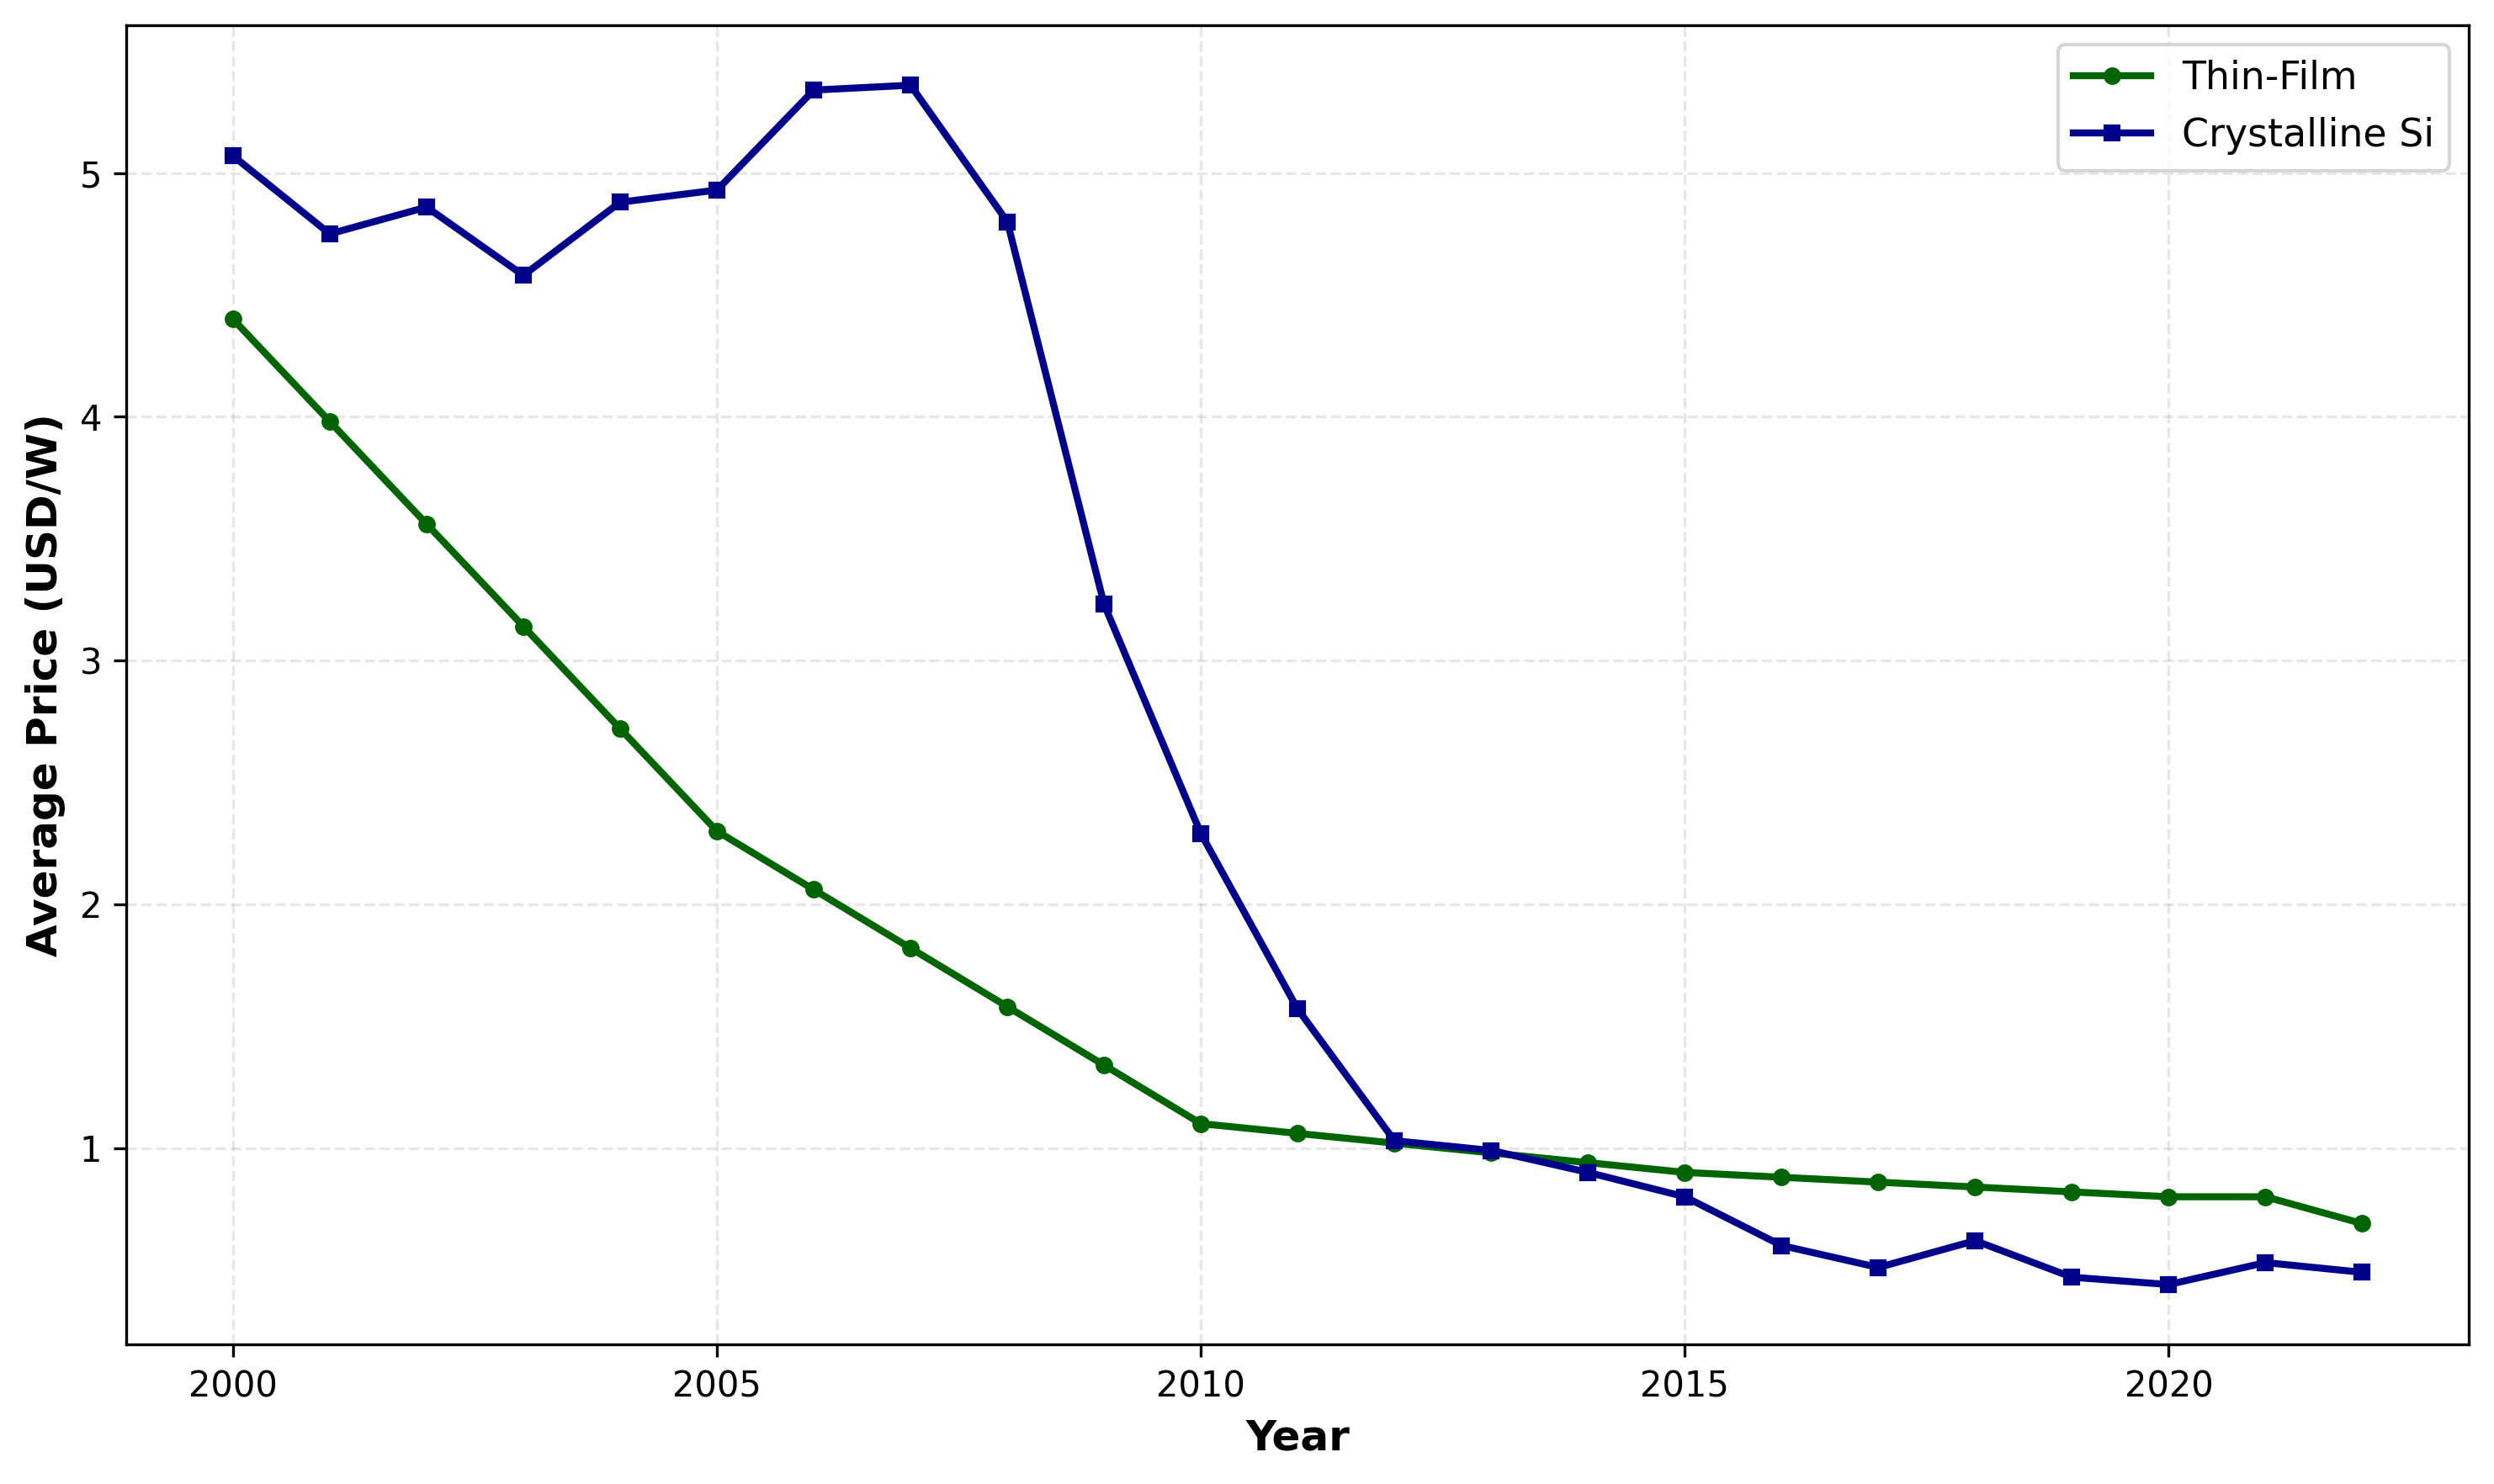
\includegraphics[width=\linewidth]{Figures/price_graph.png}
%         \caption{Price}
%     \end{subfigure}
%     \hspace{0.3cm}
%     \begin{subfigure}[t]{0.5\textwidth}
%         \centering
%         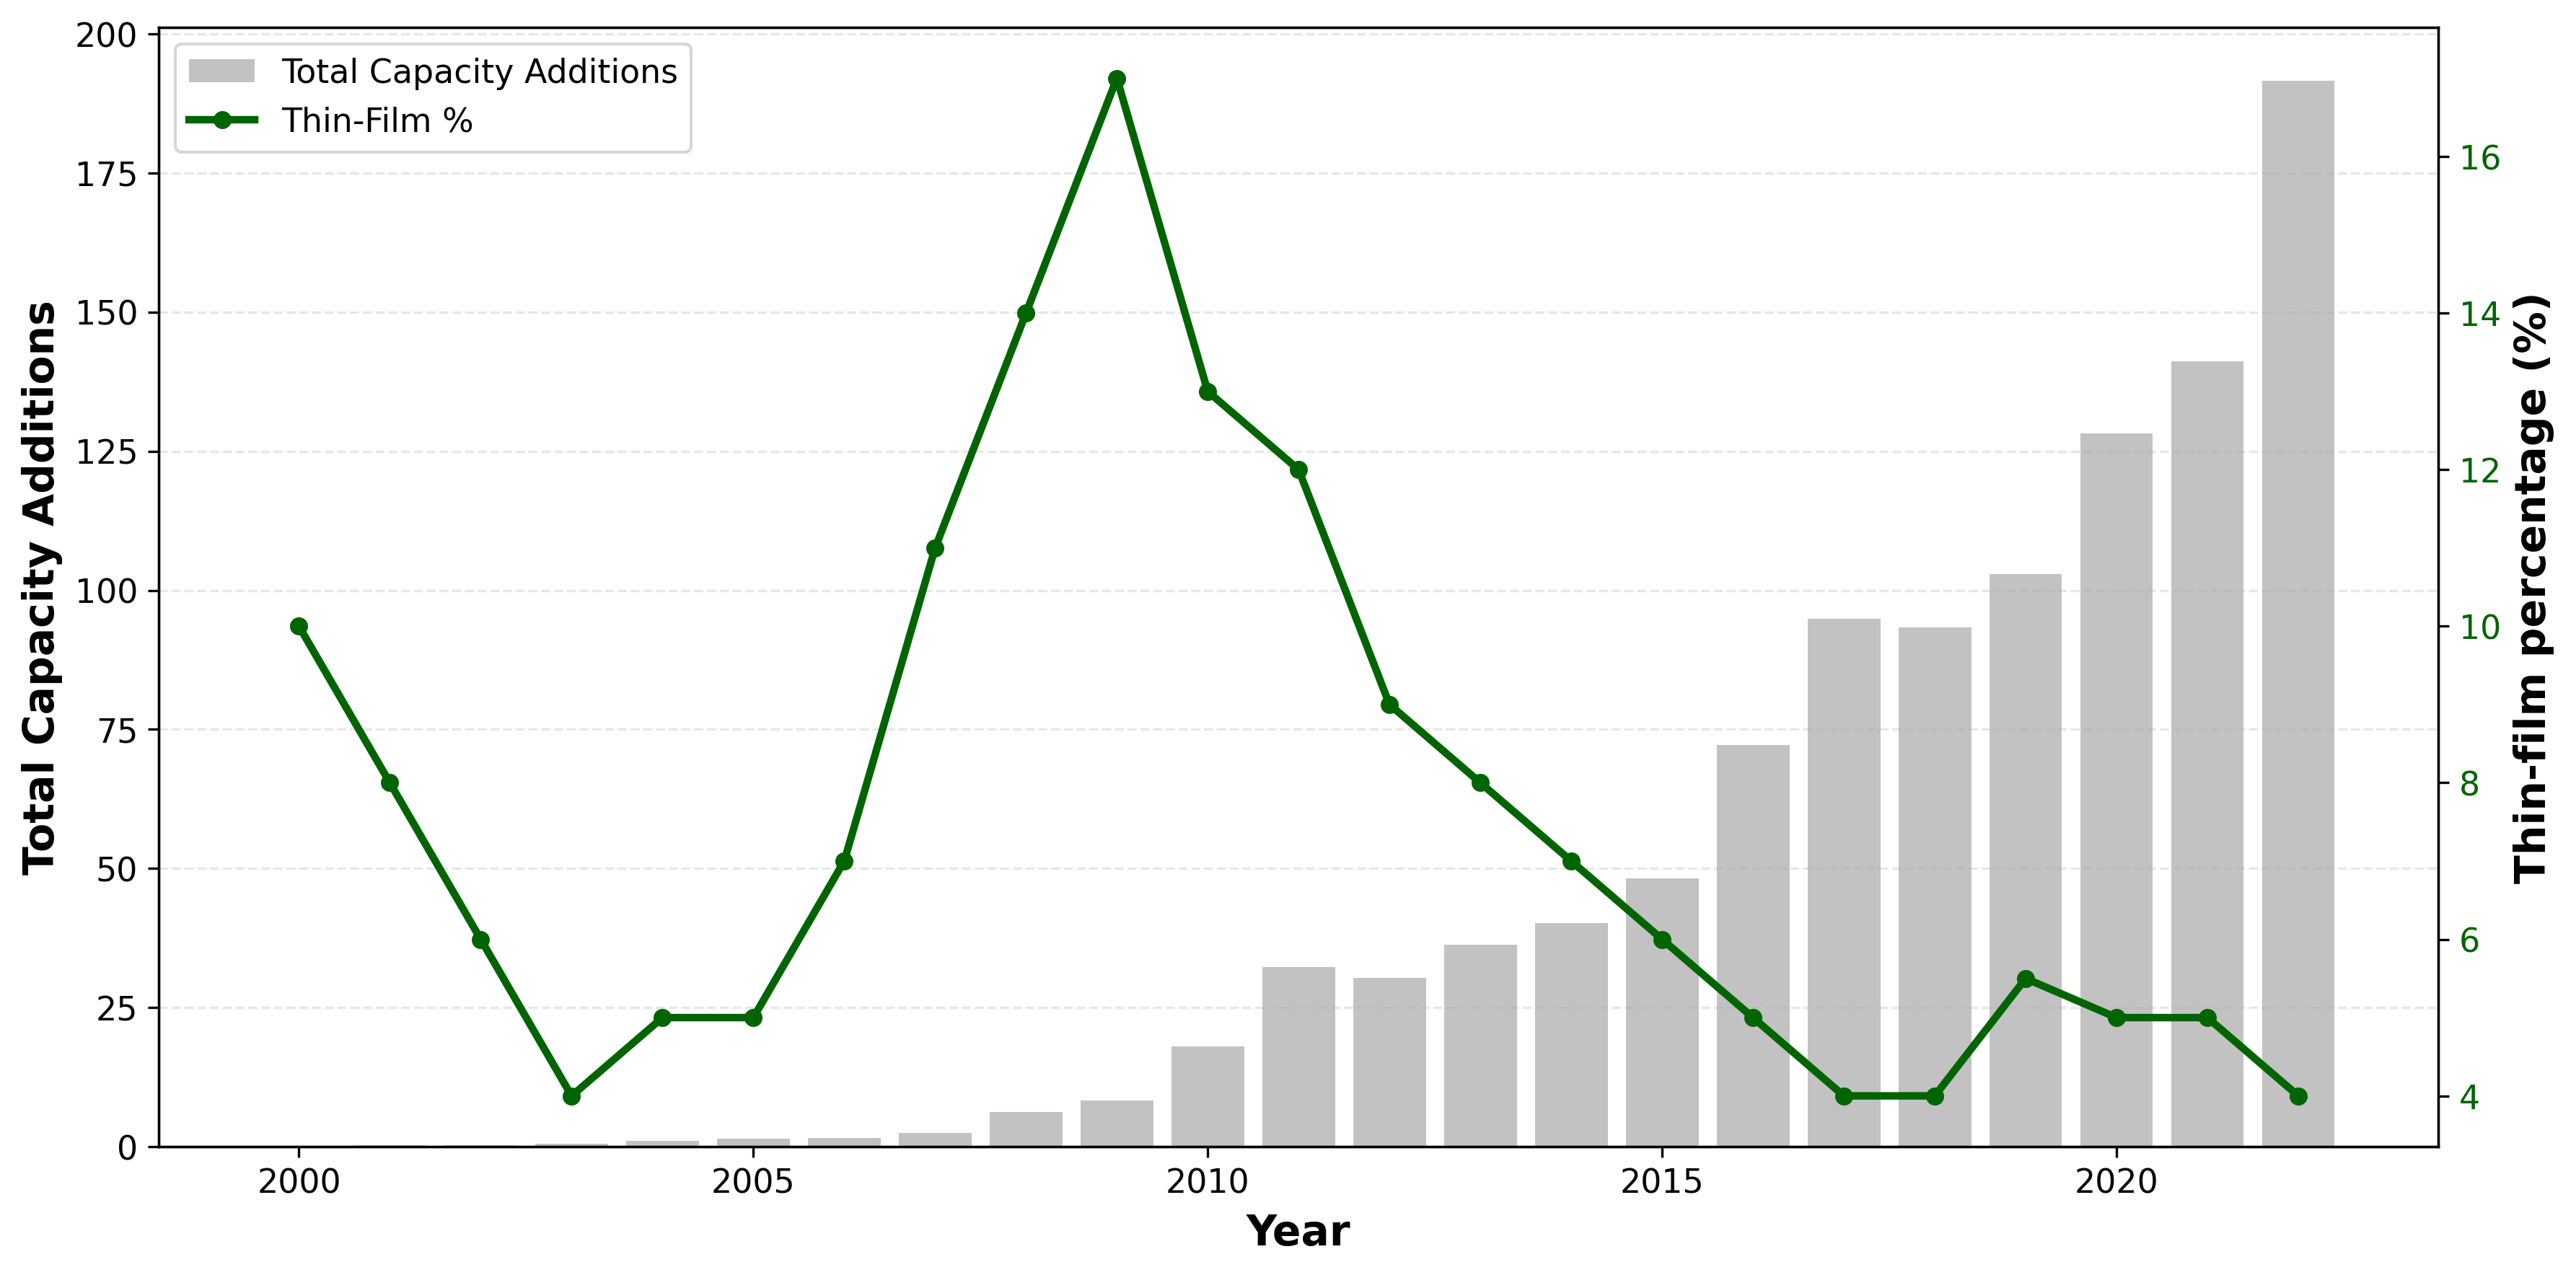
\includegraphics[width=\linewidth]{Figures/capacity_share_graph.png}
%         \caption{Installed Capacity}
%     \end{subfigure}

% \end{figure} 

\begin{figure}[tbh]
\centering
\caption{\label{fig:data_sum_two_tech_price_output}Price and Installed Capacity}
\subfloat[Price]
{\centering
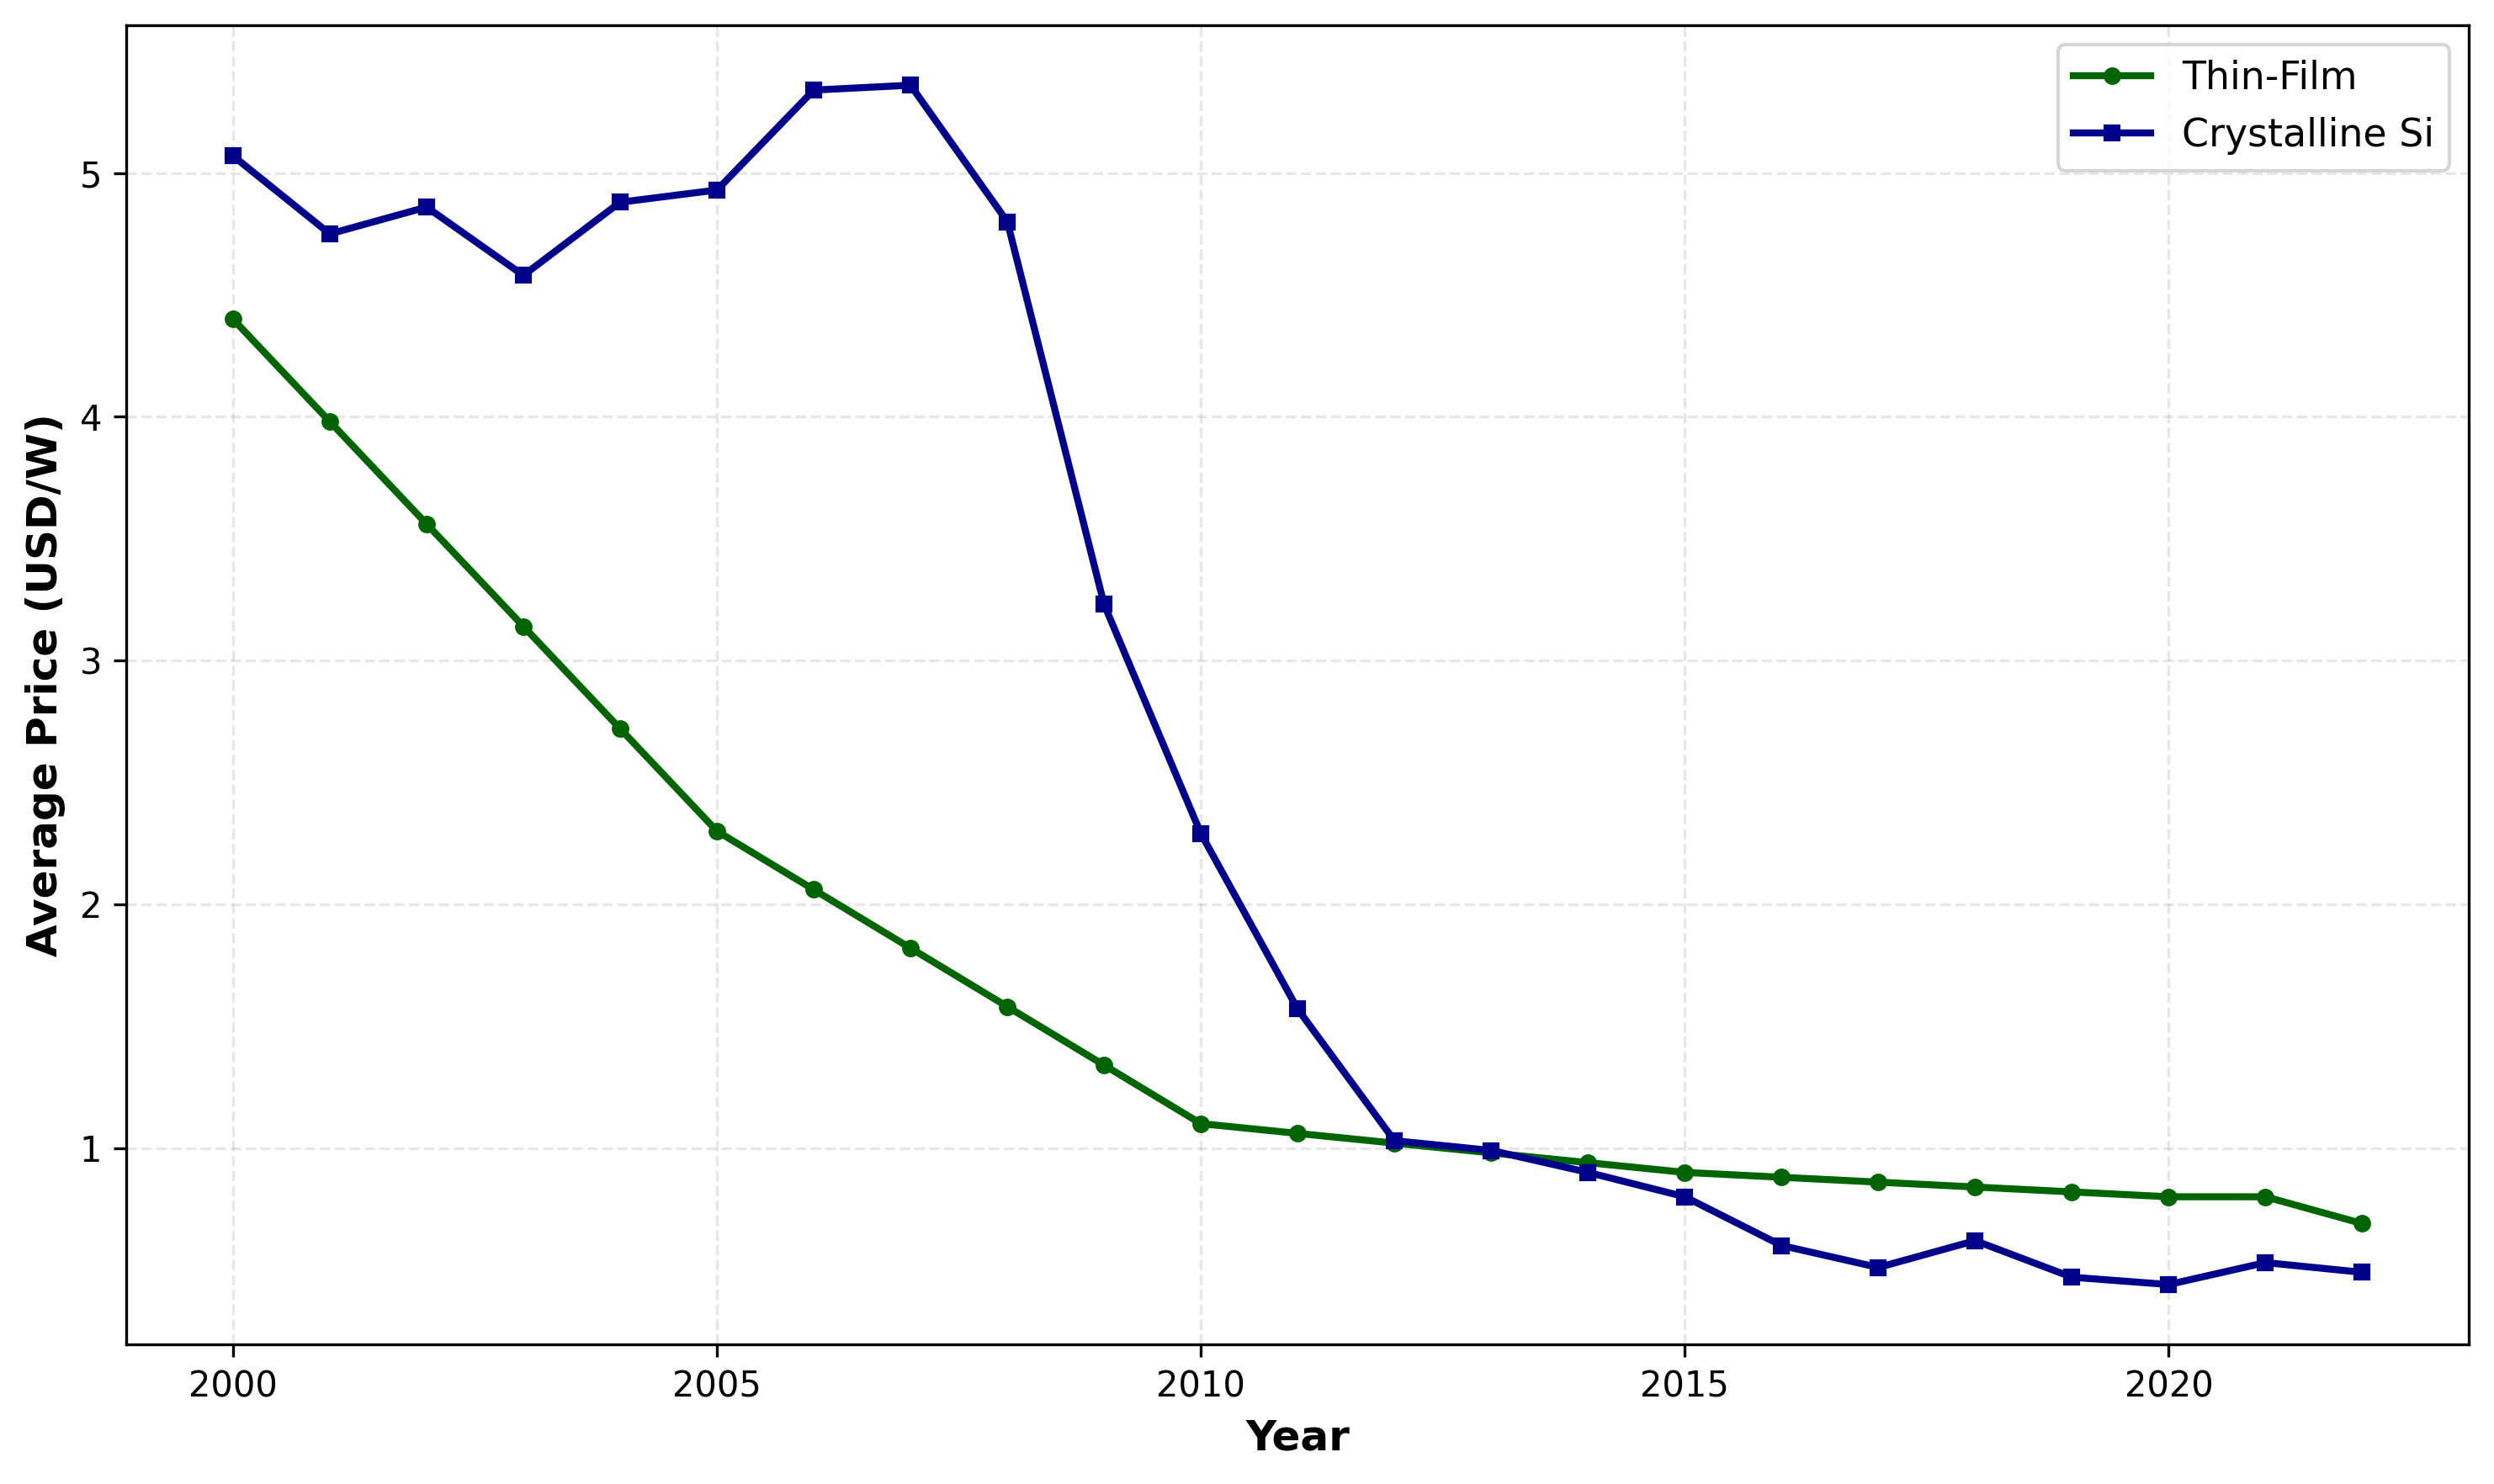
\includegraphics[scale=0.28]{Figures/price_graph.png}
}
\subfloat[Installed Capacity]
{\centering
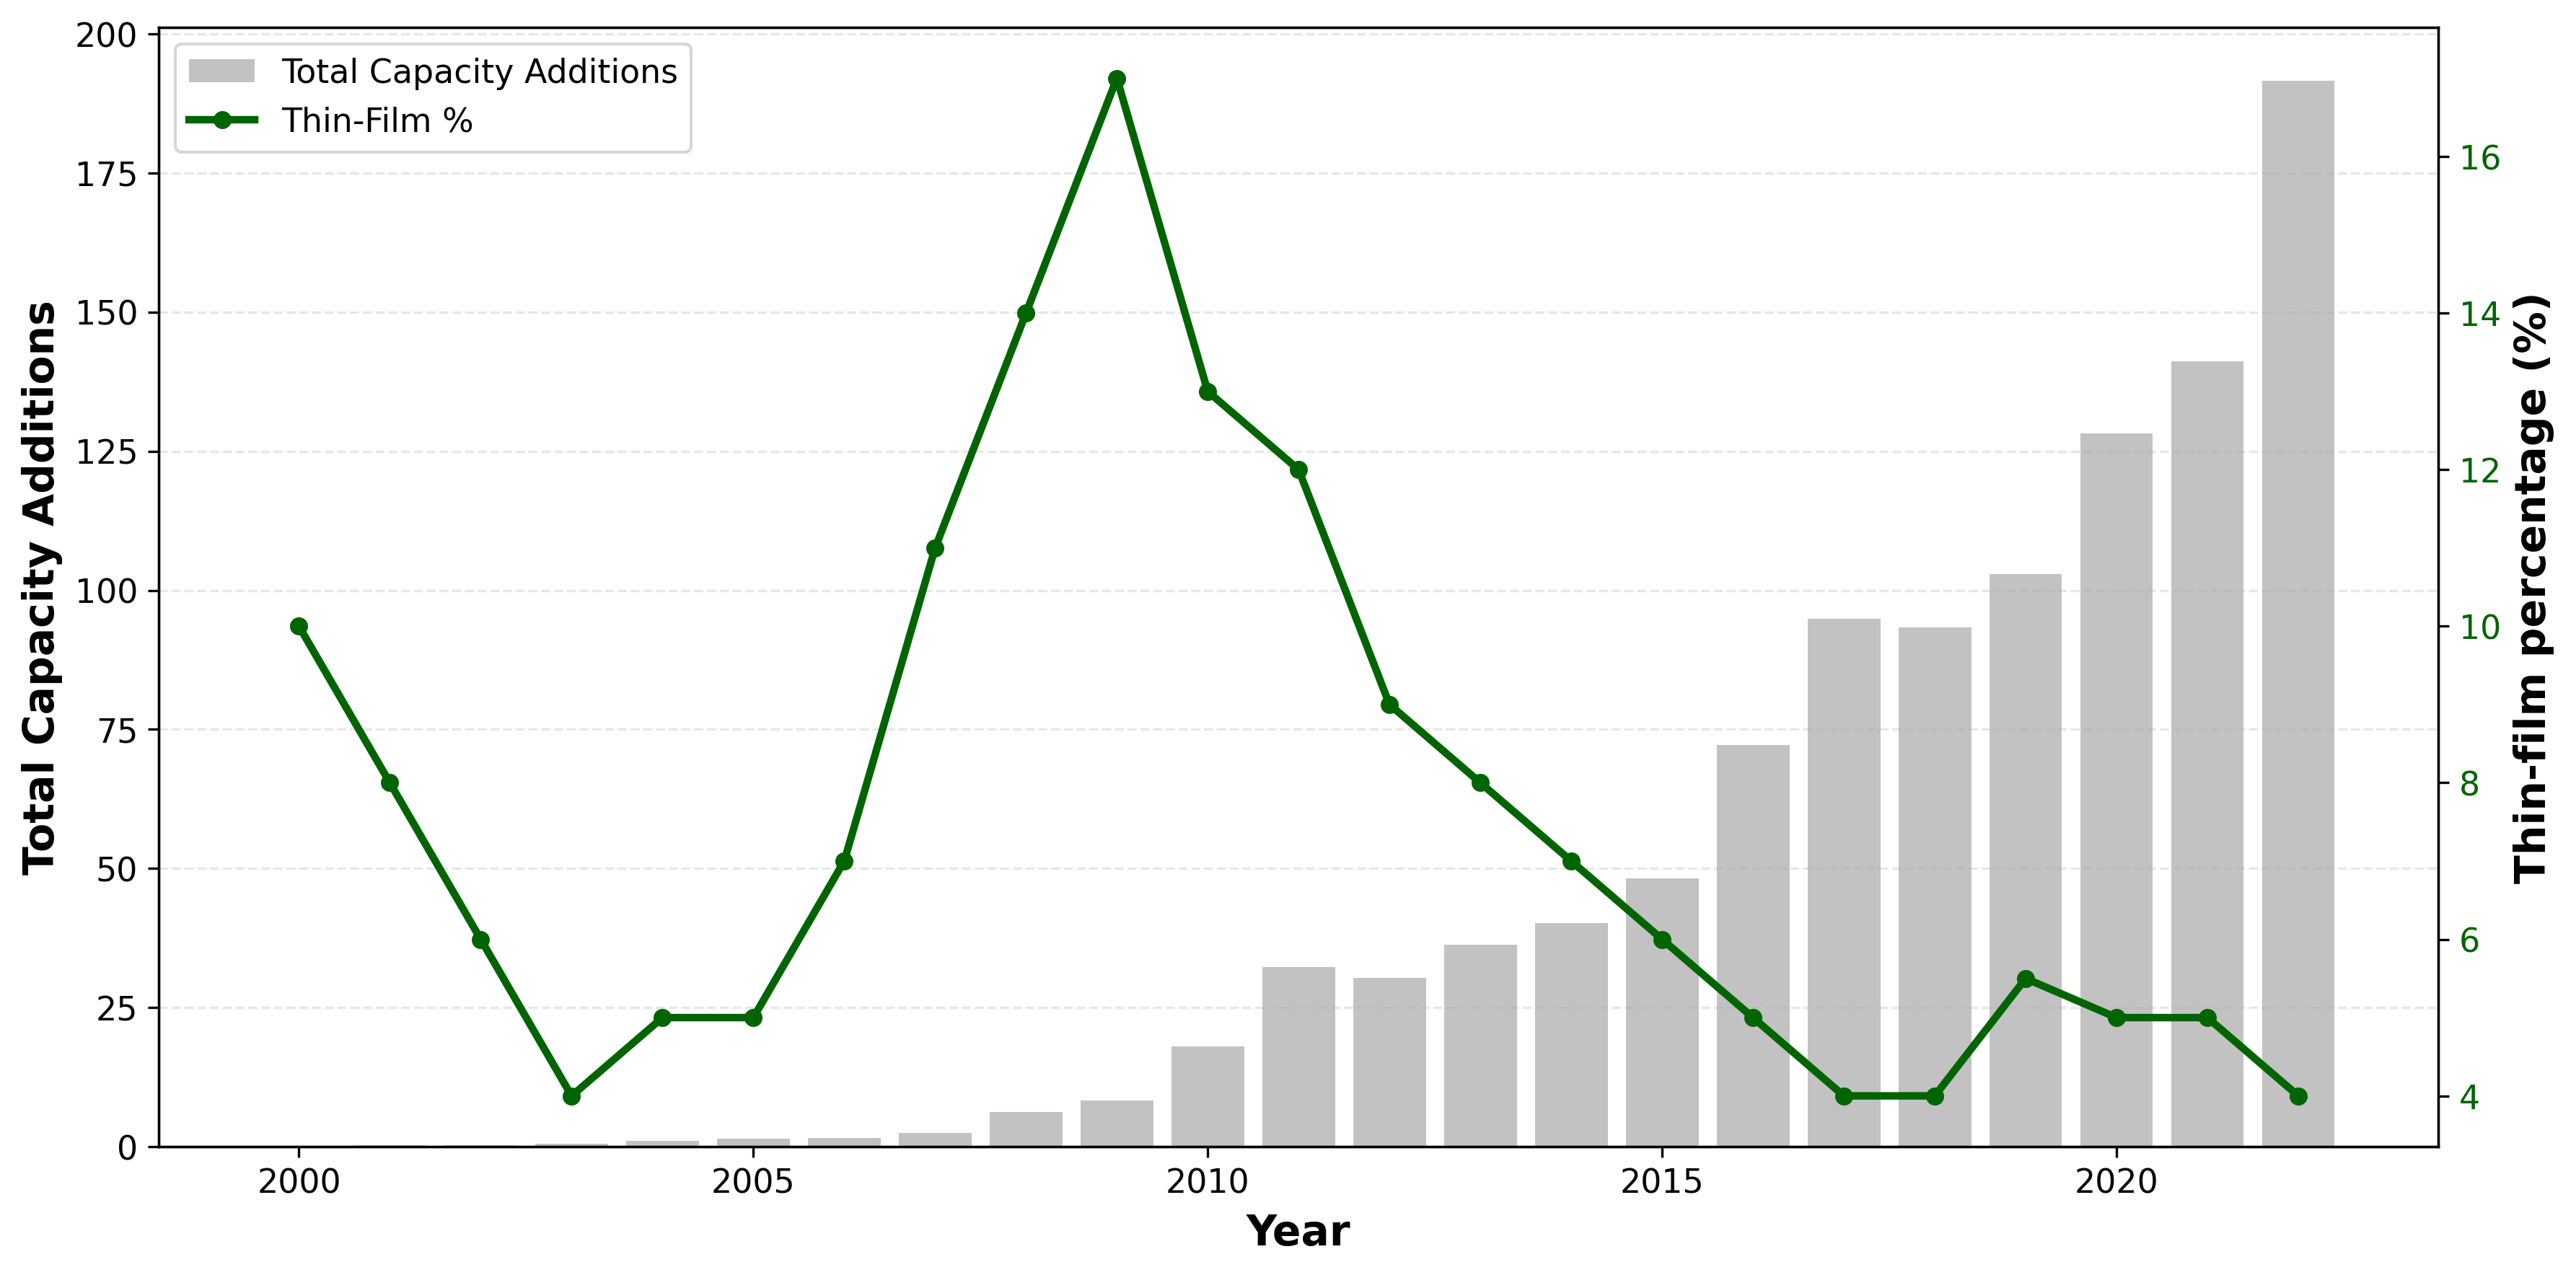
\includegraphics[scale=0.28]{Figures/capacity_share_graph.png}
}
\end{figure}

Noticeably, the price of c-Si solar panels was notably high and even rising before 2008, but it began to drop rapidly after 2008 and has remained low since. A major factor in this trend is the price of polysilicon, the main component of c-Si solar panels, which experienced a sharp increase in late 2007, as shown in Figure \ref{fig:data_sum_two_tech_input_price}(a). This surge was mainly due to the growing demand from the semiconductor sector. 
This situation led to increased investment, which do not depend on polysilicon, and the prices of the primary inputs for this type of solar panels \textcolor{blue}{remained quite stable}, as illustrated in Figure \ref{fig:data_sum_two_tech_input_price}(b).
Meanwhile, it also triggered substantial investments in polysilicon production, primarily in the U.S.. As new production came on line, along with the global recession staring in 2008, the price of polysilicon declined rapidly, falling even below pre-surge levels.  


\begin{figure}[tbh]
\centering
\caption{\label{fig:data_sum_two_tech_input_price}Price of Primary Inputs}
\subfloat[c-Si]
{\centering
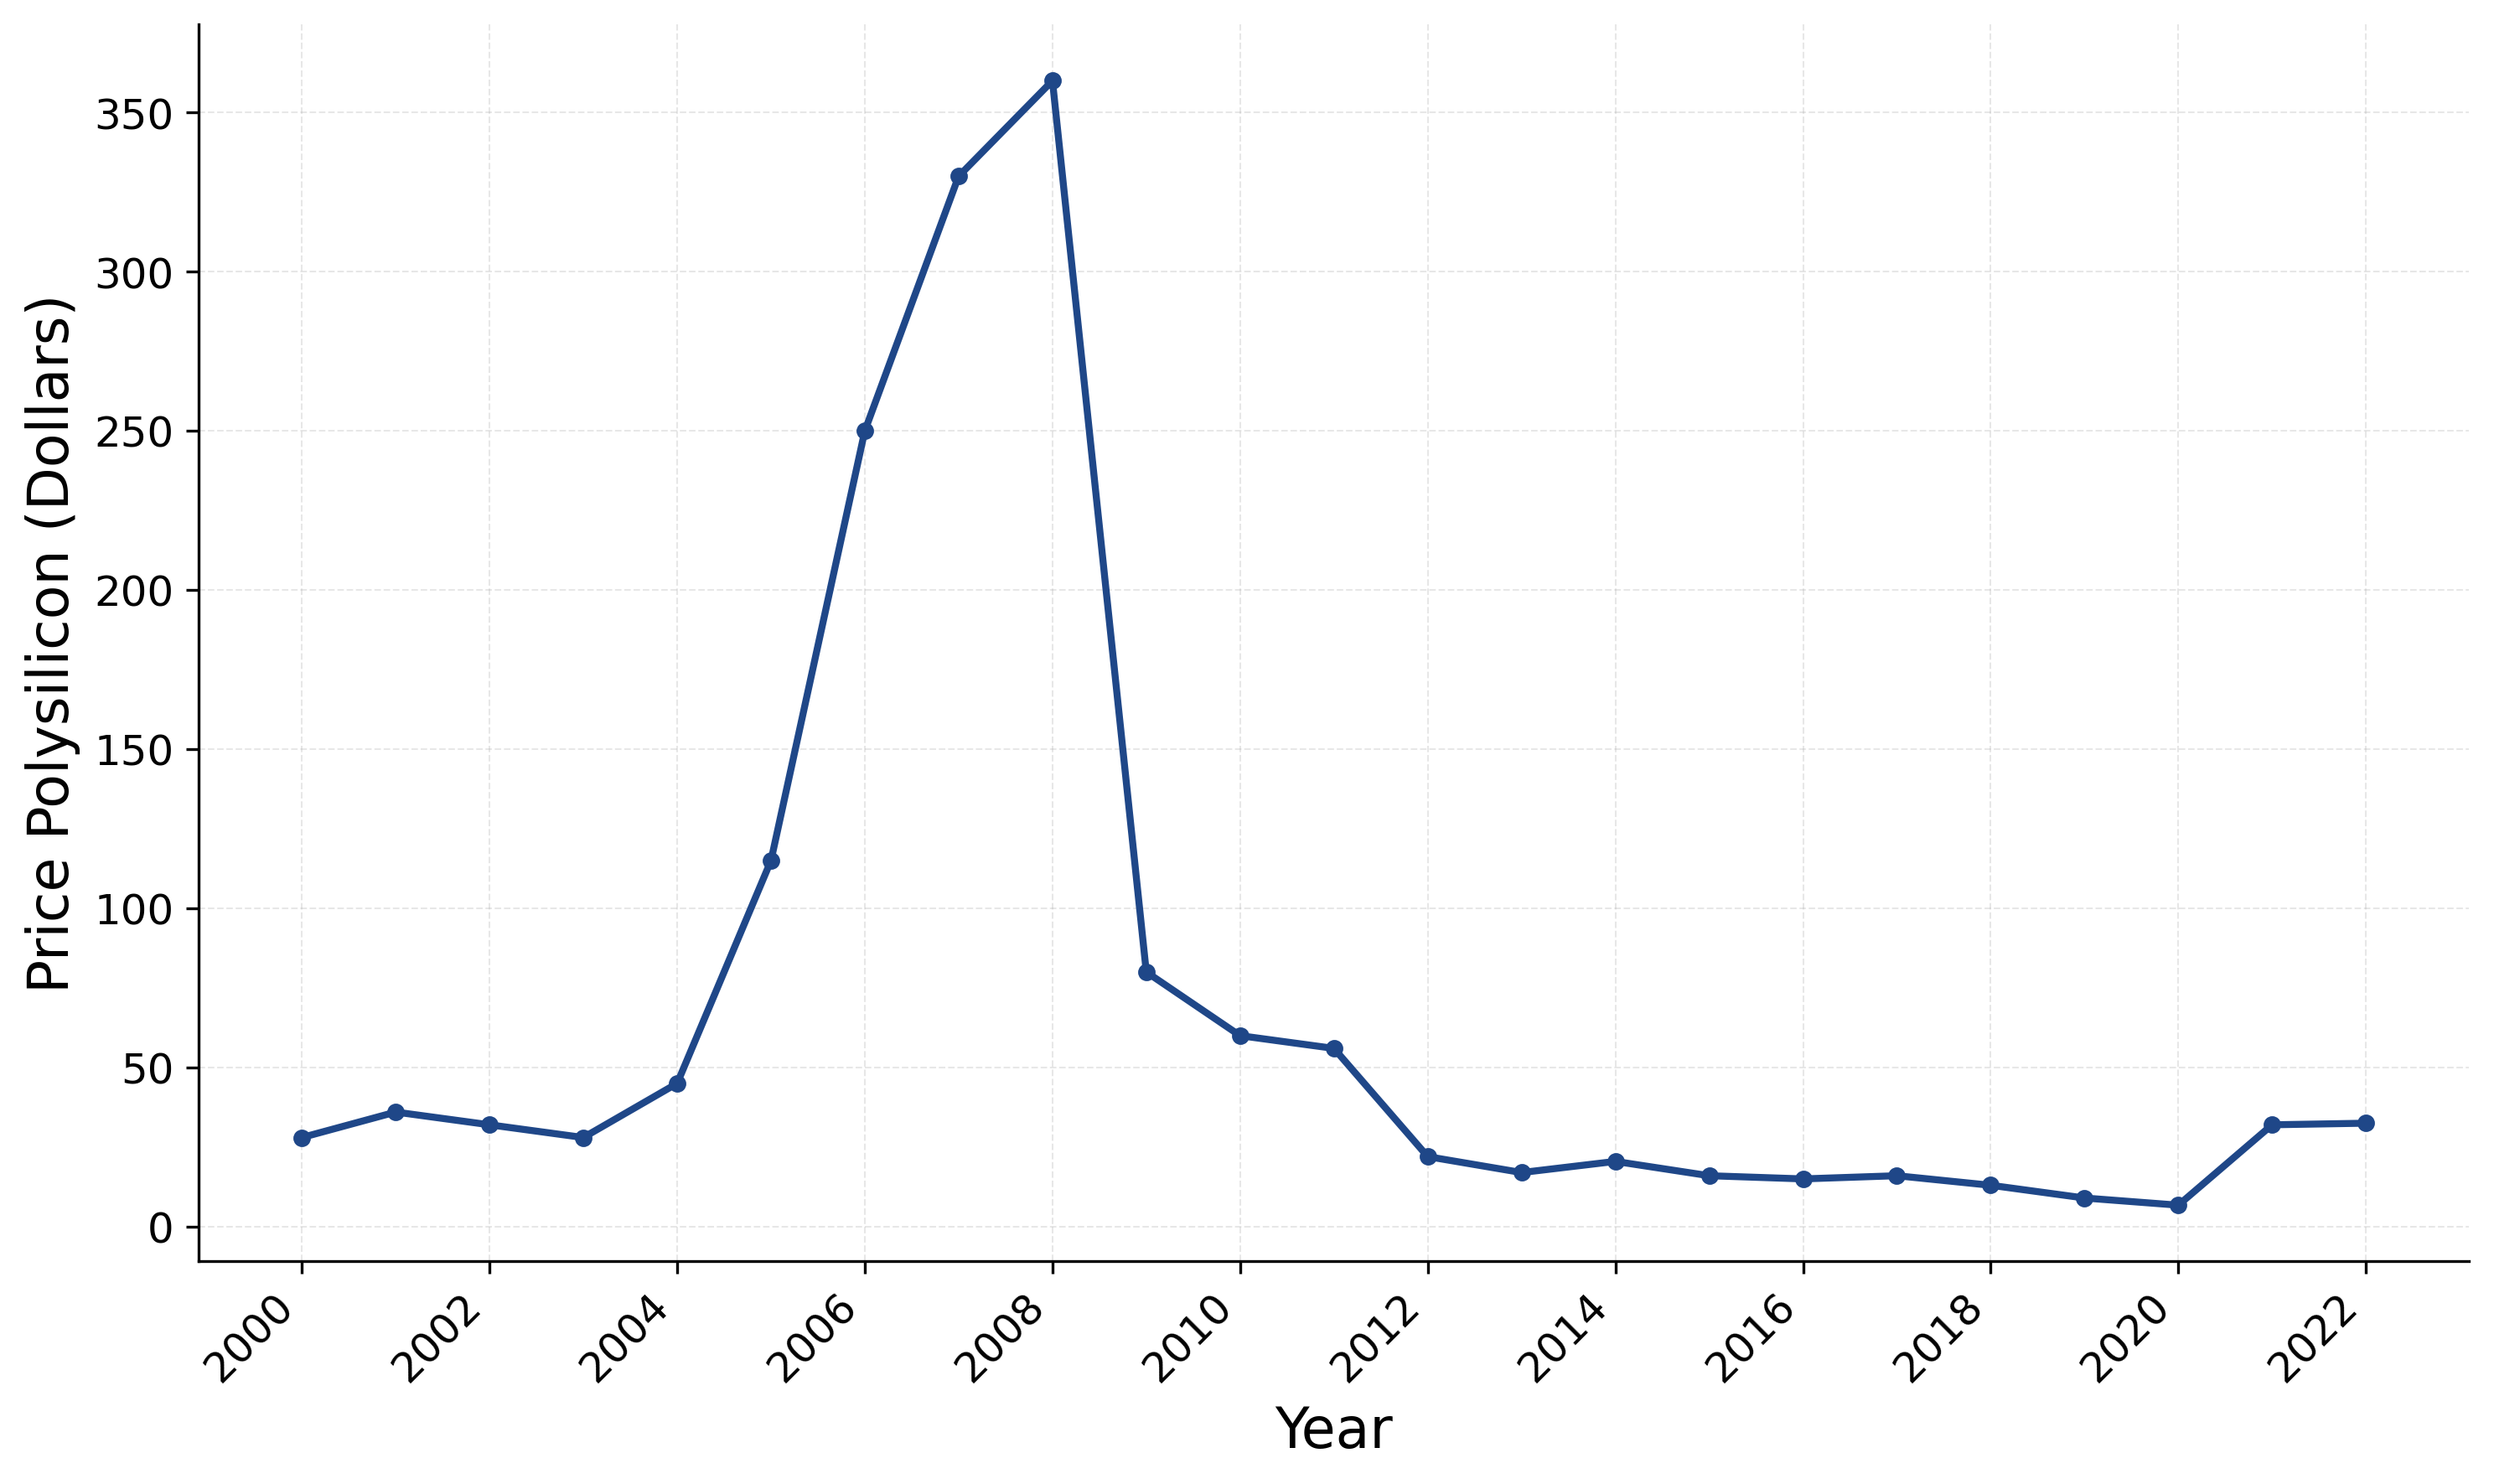
\includegraphics[scale=0.3]{Figures/polysilicon_price_series.png}
}
\subfloat[Thin-Film]
{\centering
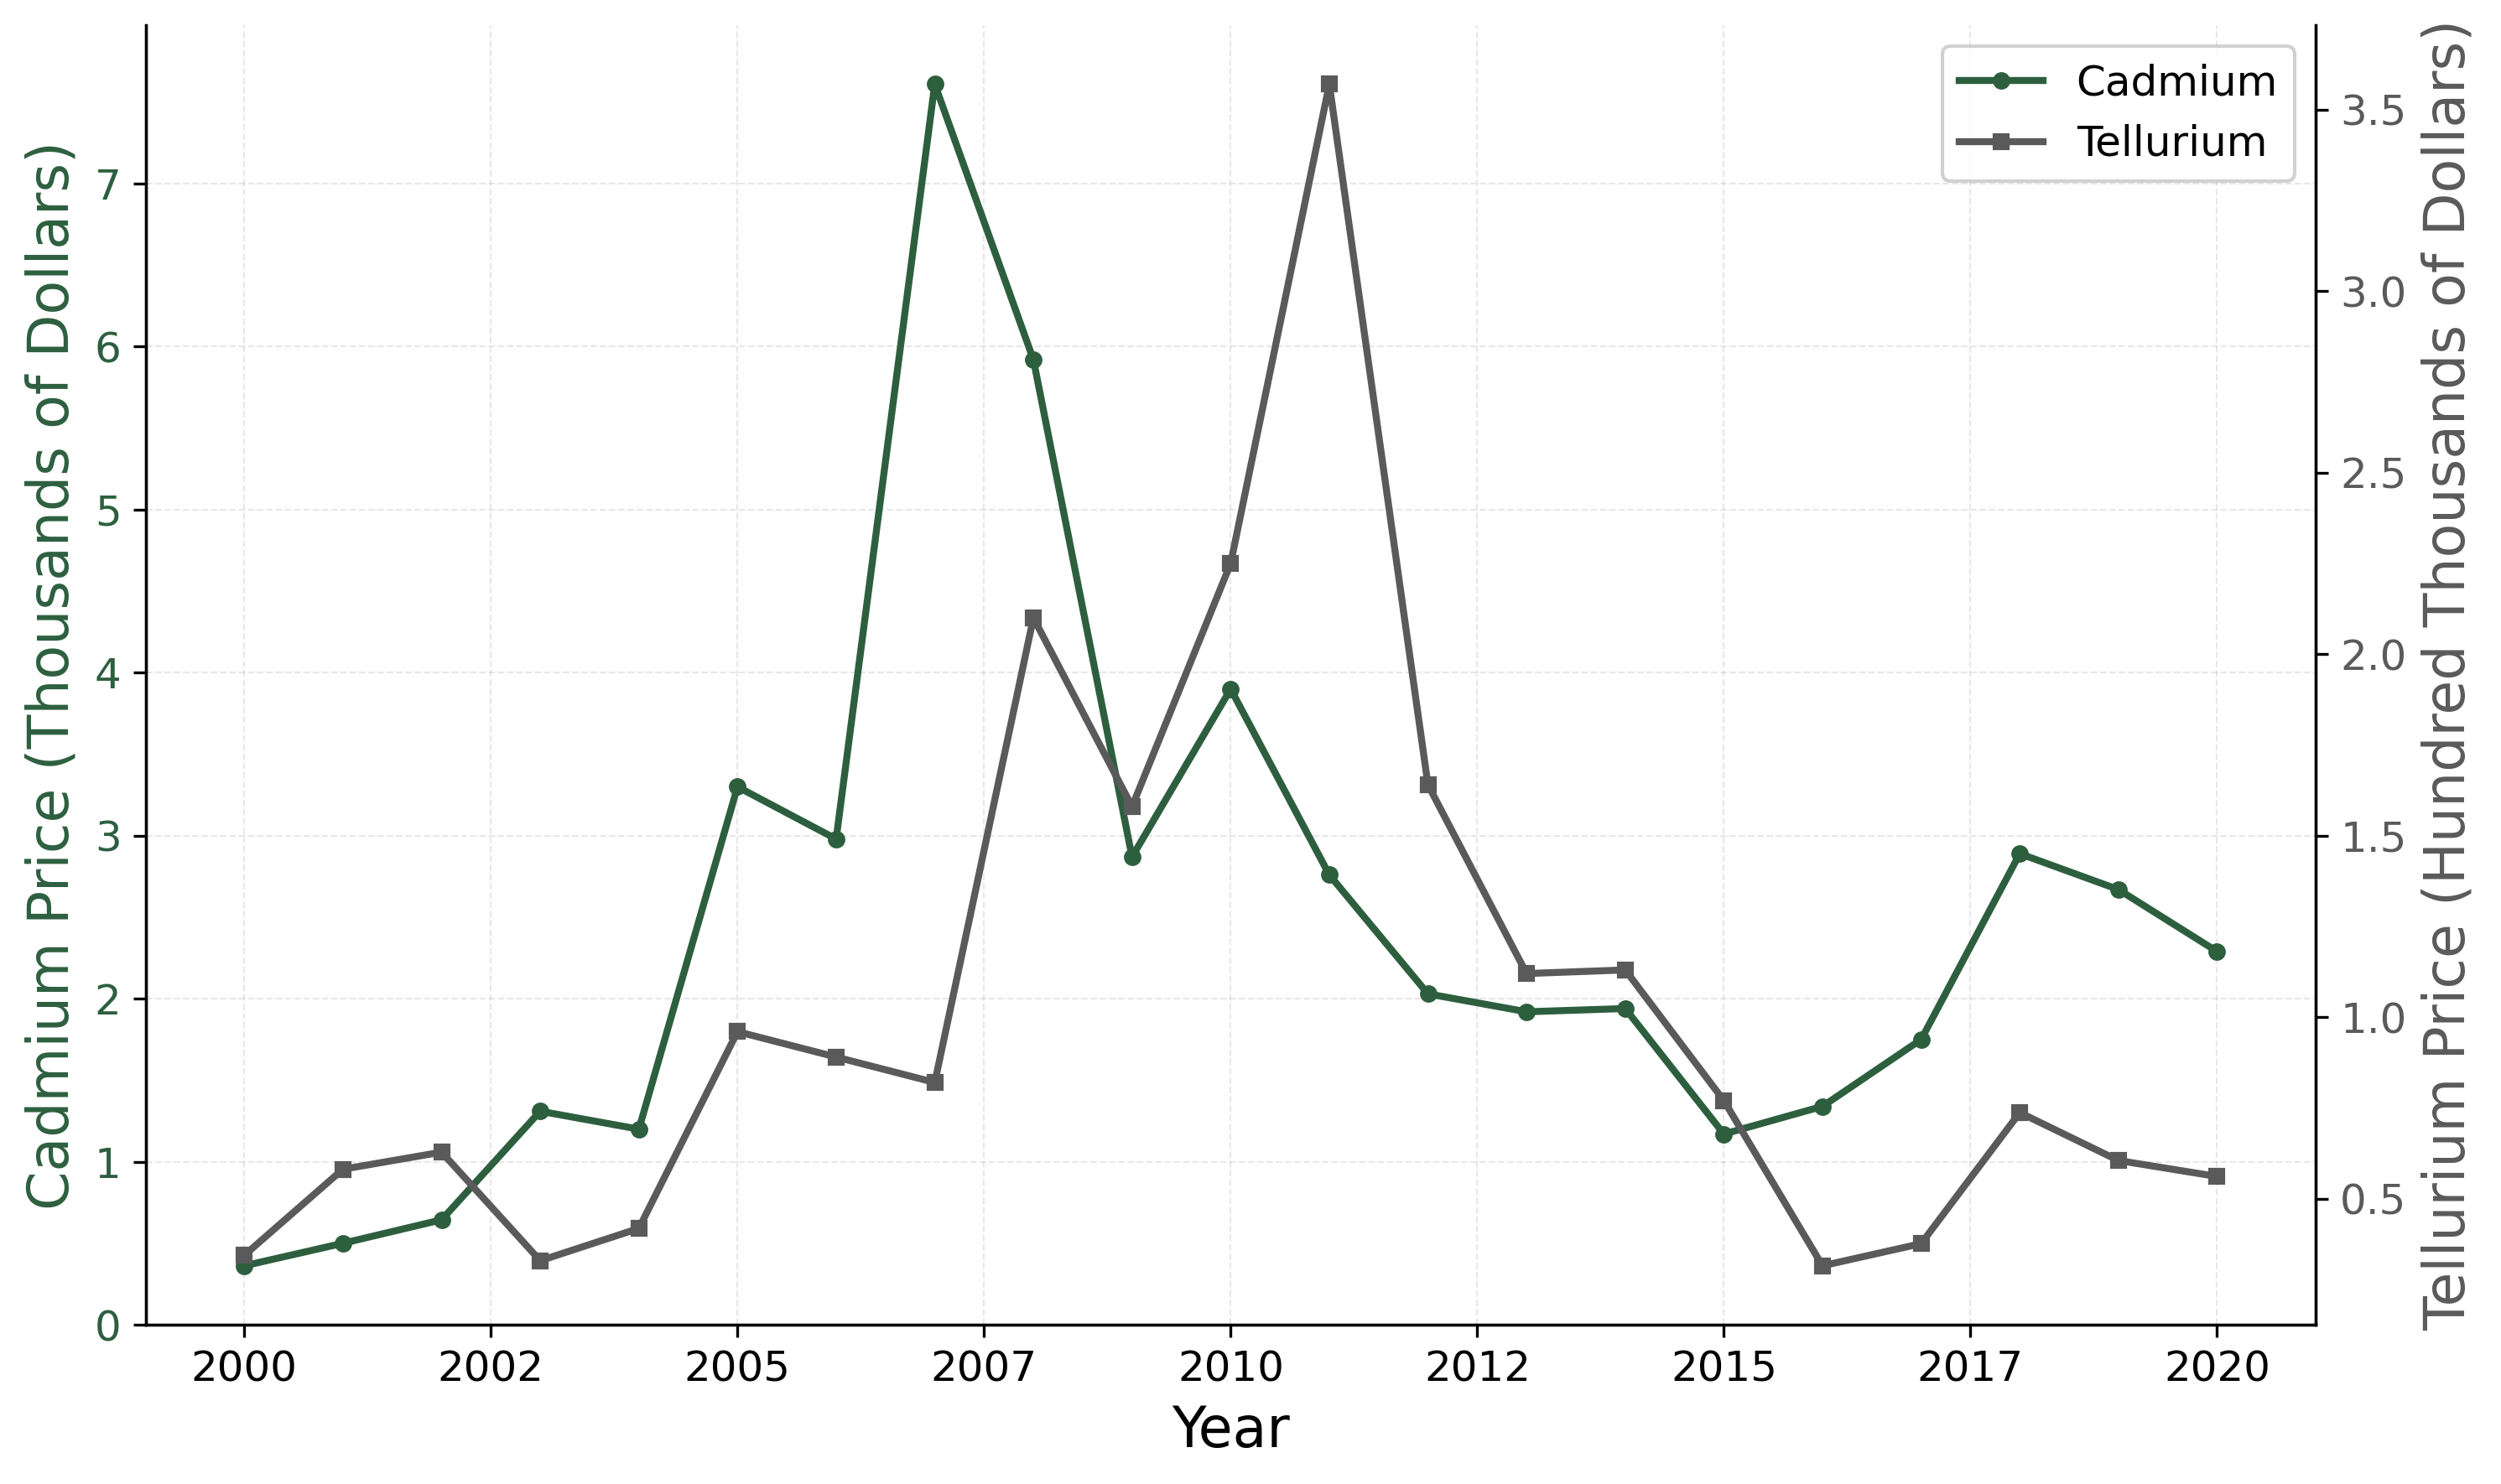
\includegraphics[scale=0.3]{Figures/cadmium_tellurium_prices.png}
}
\end{figure}

\subsection{Industrial Policies}
\label{subsec:ind_policy}
The rapid expansion of solar panel adoption is partly driven by a variety of industrial policies implemented around the world.  These policies fall into two primary categories.  The first consists of demand-side policies, designed either to encourage consumers to install solar panel systems or to discourage the use of certain types of solar panels. The second comprises production-side policies, which directly affect manufacturers' costs related to producing solar panel, as well as entering or exiting the market.

\paragraph{Demand-Side Policies}
Demand-side subsidies to encourage the adoption of solar panels have been implemented worldwide. The most widely used form is feed-in tariffs, in which governments provide a fixed payment for each unit of renewable electricity fed into the grid. These tariff rates differ substantially over time and across countries. A second form of demand subsidy is output-based support, such as net metering. A third common type of subsidy is direct payments or tax credits to cover a proportion of the upfront investment costs. 

The primary form of subsidy in the EU has been feed-in tariffs, in place since the early 2000s. For example, Germany and Spain offered solar feed-in tariffs of 40–60 cents per kWh, far exceeding the wholesale electricity prices received by other forms of electricity generations. By contrast, the primary federal demand-side subsidy in the US is the Investment Tax Credit, which provided a 30\% subsidy on upfront capital costs. In 2009, China launched the ``Golden Sun Program" to speed up the deployment of solar panel power plants, covering up to 50\% of investment costs through 2013, after which it was replaced by other policy instruments.\footnote{Further details on the program can be found in \cite{iea_golden_sun_2021}.} In addition, China implemented feed-in tariffs in 2010, with rates comparable to those offered in the EU.

The rapid decline in solar panel prices has not been without controversy. \citet{nemet2019solar} uses ``gift to the world" to refer to the dramatic production cost reductions achieved by Chinese solar panel manufacturers. However, other nations view China's dominance in solar panel manufacturing as a competitive threat. This perception is partly due to accusations of unfair trade practices and industrial policies by the Chinese government. In response, both the US and the EU have implemented a range of measures aimed at safeguarding their domestic industries since 2010. The first round of anti-dumping and countervailing duties was introduced in 2012. In addition, both the US and the EU start to impose tariffs on c-Si solar panels imported from China. Additional information on US tariffs on solar panels is provided in \citet{bollinger2025strategic}.

 The sharp drop in solar panel prices has generated considerable debate. \citet{nemet2019solar} characterizes the substantial reductions in production costs achieved by Chinese solar manufacturers as a “gift to the world.” Yet many countries regard China’s dominant position in solar panel production as a competitive threat. This concern is fueled in part by allegations of unfair trade practices and government-backed industrial policies in China. In reaction, the US and the EU have, since 2010, adopted various measures to protect their domestic industries. The first wave of anti-dumping and countervailing duties was imposed in 2012. Moreover, both the US and the EU began levying tariffs on c-Si solar panels imported from China. Further details on US tariffs on solar panels can be found in \citet{bollinger2025strategic}.
 
% In response to the surge in Chinese production, both the US and the EU have implemented a range of measures aimed at safeguarding their domestic industries since 2010.  The US enacted the first round of anti-dumping and countervailing duties in 2012. For major Chinese producers who participated in the investigations, the anti-dumping margins ranged from 18.3\% to 31.7\%, while all other Chinese producers were assigned a “PRC-Wide Entity” rate of 249.96\%. In 2014, the US expanded the duties to cover all solar panels assembled in China, irrespective of where the cells were manufactured.\footnote{Under the first Trump administration, the tariff regime was further expanded to include a broader set of countries, with a 30\% tariff imposed on crystalline silicon products from all major solar exporters to the US, pursuant to Section 201 of the Trade Act of 1974. In addition, tariffs of up to 25\% were levied on Chinese imports under Section 301 of the same Act. In 2024, the Biden administration revised and prolonged the Section 201 tariffs through 2026 and raised the ad valorem rate on Section 301 tariffs from 25\% to 50\%.} For comparison, the EU launched its initial round of anti-dumping investigations into Chinese solar manufacturers at roughly the same time as the US and subsequently imposed anti-dumping duties on major cooperating Chinese producers ranging from 27.3\% to 64.9\%, as well as a 53.4\% rate on other “PRC-Wide Entity” producers. In 2018, the EU lifted both the anti-dumping tariffs and the minimum import price requirements applied to Chinese producers.

% They initiated multiple anti-dumping investigations against Chinese manufacturers and imposed tariffs on solar cells manufactured in China.

% The US enacted the first round of US anti-dumping and countervailing duties in 2012. For major Chinese producers who participated in the investigations, the anti-dumping margins ranged from 18.3\% to 31.7\%, while all other Chinese producers were assigned a “PRC-Wide Entity” rate of 249.96\%. In 2014, the US implemented a second round of tariffs to address loopholes in the 2012 measures, expanding the duties to cover all solar panels assembled in China, irrespective of where the cells were manufactured. Under the first Trump administration, the tariff regime was further expanded to include a broader set of countries, with a 30\% tariff imposed on crystalline silicon products from all major solar exporters to the US, pursuant to Section 201 of the Trade Act of 1974. In addition, tariffs of up to 25\% were levied on Chinese imports under Section 301 of the same Act. In 2024, the Biden administration revised and prolonged the Section 201 tariffs through 2026 and raised the ad valorem rate on Section 301 tariffs from 25\% to 50\%.

% The EU launched its initial round of anti-dumping investigations into Chinese solar manufacturers at roughly the same time as the US and subsequently imposed anti-dumping duties on major cooperating Chinese producers ranging from 27.3\% to 64.9\%, as well as a 53.4\% rate on other “PRC-Wide Entity” producers. In 2018, the EU lifted both the anti-dumping tariffs and the minimum import price requirements applied to Chinese producers.

%\textcolor{blue}{[Insert two graphs. Graph (a) displays the weighted average feed-in-tariffs for each region for the years panning from 2000 to 2013. Graph (b) displays the tariff rate imposed by US and EU on Chinese solar panels during this period.]}

\paragraph{Production-Side Policies} Direct subsidies to producers are relatively limited in the EU and the US,\footnote{Some manufacturers have benefited from targeted subsidies, such as R\&D loans or funding to renewable energy.} but are prevalent in many emerging economies, especially in China. 
China supported the solar panel manufacturing industry through an extensive range of policy instruments. During the initial growth phase, most of solar panel production subsidies were granted by provincial and local government. These took the form of reduced land prices or rents, low-interest loans, tax exemptions, and decreased electricity rates.\footnote{For example, Suntech in Jiangsu  benefited from \$3.7 billion in low-interest loans from a state-owned bank and an additional \$1.4 billion in tax rebates and other export support subsidies from 2005 to 2012, as noted in \cite{urban2016solar}.}

During the later stage of the surge, the central government stepped in. In 2010, the State Council declared solar panel as more than just renewable energy, labeling it a ``strategic emerging industry". State-owned banks supported this industry by extending billions of dollars in credits, as mentioned in \cite{lexology2010strategic} and \cite{nahm2023state}. The central government also supported the creation of a domestic silicon industry, although the initial goal was to supply inputs for semiconductors instead of solar panels. According to data from \cite{waferpro_2024_china_silicon_supply}, China's polysilicon production surged from 6,000 Metric Tons in 2000 to 410,000 in 2019. %However, China was still a major importer of polysilicon before 2024, as noted by \cite{solarbe_2024_global_polysilicon}. The subsidization of polysilicon shielded Chinese solar panel manufacturers from the industry shortages that affected other nations, as mentioned in \cite{bernreuter_2020_polysilicon_market_analysis}.

However, systematic data on the quantitative impact of production-side industrial policies is still scarce. Since these policies cannot be directly measured in practice, we follow an indirect strategy: we use detailed firm-level data on production and entry/exit to infer the implied subsidies on production and entry costs by assuming that the observed decisions arise from the equilibrium of a suitably specified model. This methodology has been employed, among others, by \citet{barwick2025industrial} in their analysis of the Chinese shipbuilding industry.


\subsection{Data}
\label{subsec:inst_data}

Our analysis combines data from multiple sources spanning the years 2000 to 2013. 

\paragraph{Chinese Solar Panel Export Volumes}
The first source is the \textit{Chinese Customs Transactions}, which contains the quantity and trade value of all Chinese solar panel export transactions. Using this dataset, we construct export volumes at the firm–destination–year level. For the empirical analysis, we group export destinations into five regions: the EU, India, Japan, the US, and the Rest of the World (ROW).

\paragraph{Chinese Solar Panel Manufacturers}
The second data source is the \textit{Annual Survey of Manufacturing}, an annual survey administered by the Chinese National Bureau of Statistics that provides detailed information on the manufacturing firms surveyed. This dataset has been used in various academic studies, including \citet{roberts2018role} on the footwear industry and \citet{barwick2025industrial} on shipbuilding, among others. \textcolor{blue}{[Some description about how we identify solar panel manufacturing firms.]} For each manufacturer in each year, the survey reports its output, total fixed assets, and a set of time-varying characteristics, such as location (province), ownership status (whether it is state-owned, privately owned, or foreign firm), and the year in which the firm was established.  Using data on total fixed assets, we construct measures of capital stock and investment following the methodology in \citet{brandt2012creative} and \citet{barwick2025industrial}.

\paragraph{Regional-Level Solar Panel Installation and Demand Incentives}
We obtain quarterly information on the solar panel installation for each technology for each of the six economic regions -- China, EU, India, Japan, US, and ROW -- based on data from \cite{OWID_solar_pv_capacity_2025} and \textcolor{blue}{percentages drawn from various news and literature sources cite}. In addition, we collect information on demand subsidy policies in each economic region, including tax credit or rebates, feed-in tariff rates, and import tariff rates on c-Si solar panels. The data on tax credits and rebates and feed-in tariff rates is sourced from \textit{IEA's database} and also \cite{gerarden2023demanding}.

\paragraph{Prices of Solar Panel and Inputs for each Technology}
We obtain the quarterly global price per Watt for each of the two technologies, along with the quarterly global price for Polysilicon and the annual prices for Cadmium, and Tellurium. The quarterly Polysilicon price data is sourced from \textit{Bloomberg New Energy Finance} and \textit{Bernreuter Research}, while the annual prices of Cadmium, Tellurium, silver, and aluminum are obtained from the \textit{United States Geospatial Services (USGS)}. 

\paragraph{Auxiliary Data}
We supplement our main data with several auxiliary data. First, we compile aggregate annual production figures for the two solar panel technologies in regions outside China over the sample period. Second, we collect socioeconomic variables (such as GDP and total electricity consumption) for each economic region. Third, we obtain the global prices for key inputs used in the two solar panel manufacturing technologies, including polysilicon, cadmium, and tellurium.


\subsection{Descriptive Evidence}
\label{subsec:inst_china_PV}

Figure \ref{fig:data_sum_China_output}(a) presents China's production of the two solar panel technologies and its share in the global market.
China's solar panel manufacturing industry was miniscule in the early 2000s. 
The cell production was 3 megawatts (MW) in 2000, accounting for less than 2 percent of global output. China’s share then jumped to 14 percent in 2006 and grew fast over the following five years. By 2011 it reached 60 percent and has remained above that level ever since. The figure also shows that China’s solar panel manufacturing is dominated by c-Si technology, whereas the global share of thin-film fluctuates over time, particularly in response to changes in polysilicon prices, as shown in Figure \ref{fig:data_sum_two_tech_price_output}(b).
%The cell production was 3 megawatts (MW) in 2000 according to \cite{EarthPolicy_indicator12_solar_2000_2013}, accounting for less than 2 percent of global output. It is evident that China’s expansion accelerates after 2005 and is concentrated primarily in c-Si technology.

Figure \ref{fig:data_sum_China_output}(b) displays the number of new entries, exits, and active solar panel firms in China during this time period. It indicates that a massive wave of new solar panel firm entries occurred after China declared solar panel as a ``strategic emerging industry" in 2010. New entries jumped to 118 in 2010 and remained above 50 in subsequent years. At the same time, a comparable volume of firm exits kept the total number of active firms relatively stable at about 200. 

As illustrated in Figure \ref{fig:data_sum_two_tech_price_output}(a), solar panel prices stayed high in the early 2000s, reached a peak in 2007, started to fall after 2008, and remained low from 2011 onward. In contrast, China's production grew steadily before 2009 and then accelerated after 2010, closely aligning with the timing of major industrial policy rollouts.

%China’s solar panel manufacturing industry was miniscule before 2005.  It breached 100 megawatts (MW) of cell production in that year, jumping to 7 percent of global supply from less than 2 percent in 2003. Production grew by an order of magnitude in the next two years, another order of magnitude in the following three, and doubled again in 2011, capping roughly 200x growth in a six-year span. China’s share of the global market had surpassed 60 percent by 2011, and it has remained above that level since then.


\begin{figure}[tbh]
\centering
\caption{\label{fig:data_sum_China_output}China's Market Share and Number of Firms}
\subfloat[Market Share]
{\centering
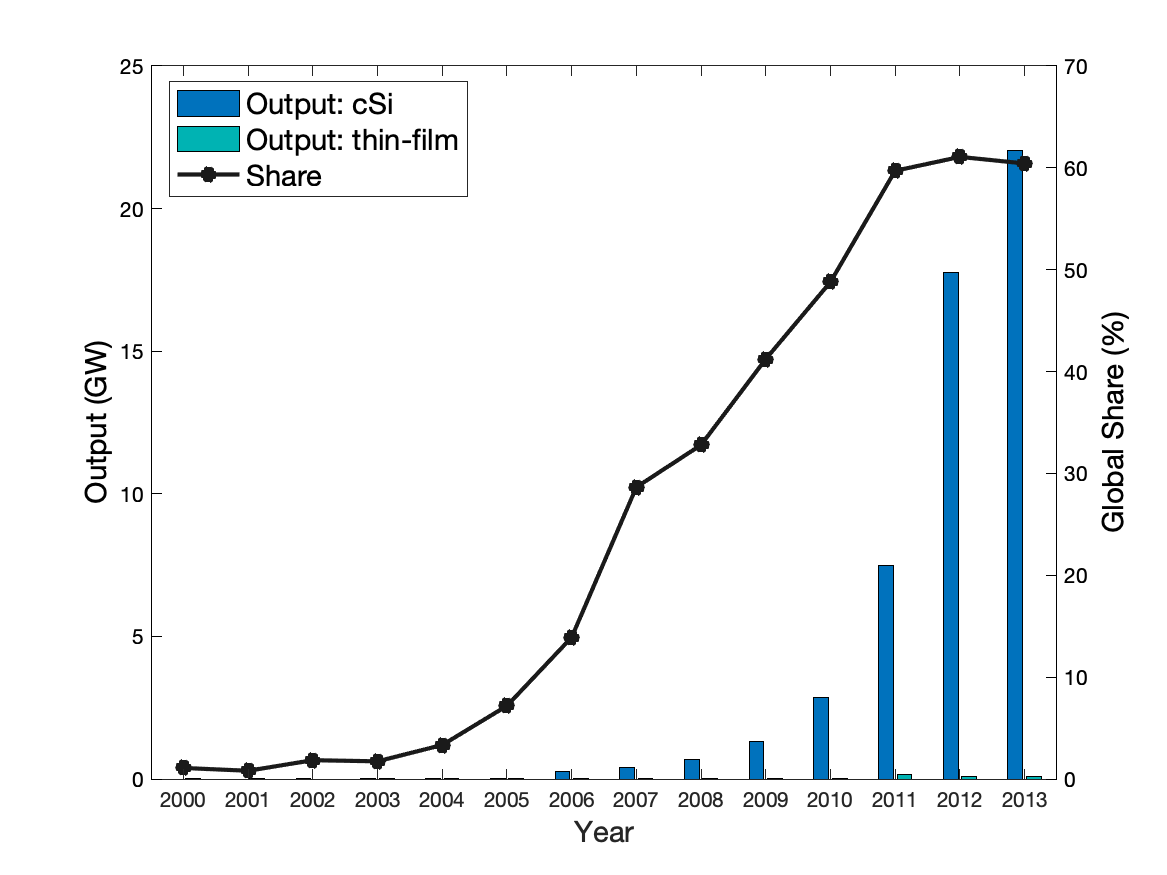
\includegraphics[scale=0.4]{Figures/Fig_data_sum_mkt_share.png}
}
\subfloat[Number of Firms]
{\centering
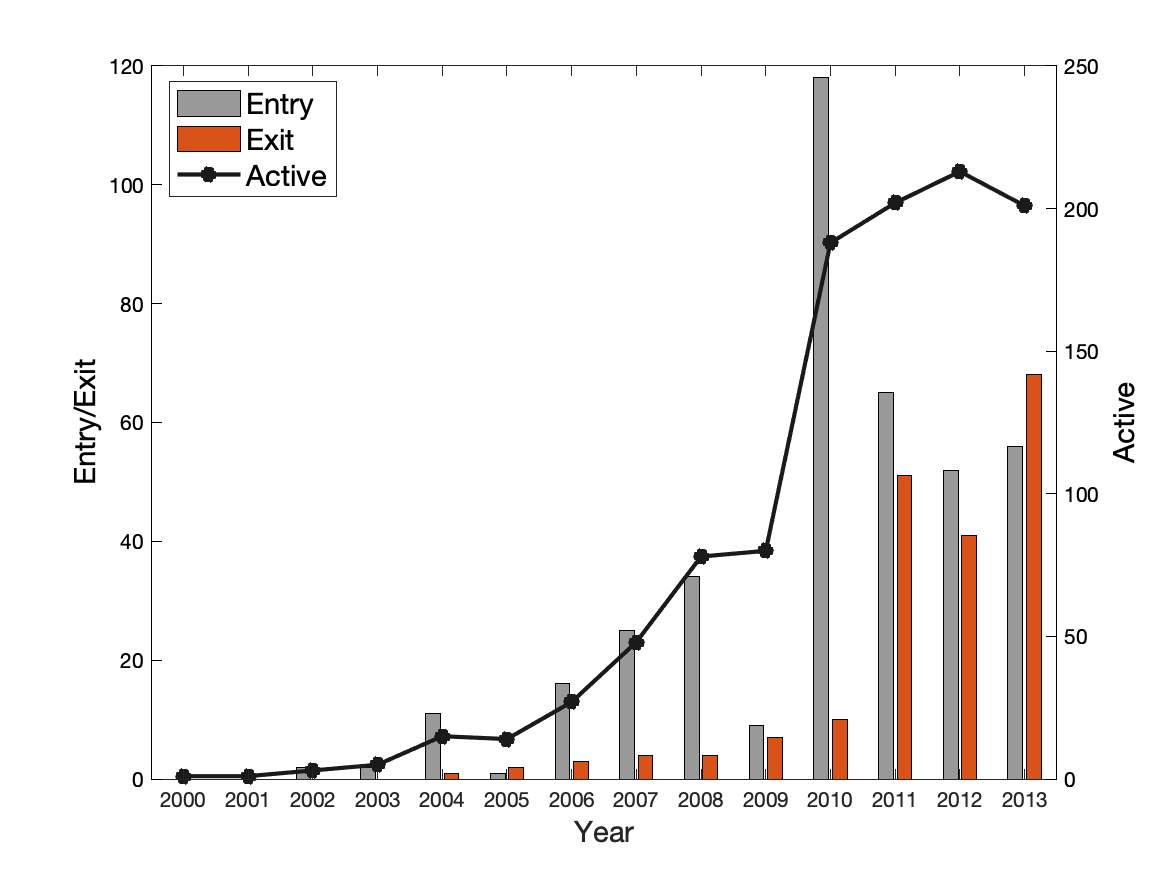
\includegraphics[scale=0.4]{Figures/Fig_data_sum_num_firms.png}
}
\end{figure}


% China supported the solar panel manufacturing industry through an extensive range of policy instruments. During the initial growth phase, most of solar panel production subsidies were granted by provincial and local government. These took the form of reduced land prices or rents, low-interest loans, tax exemptions, and decreased electricity rates. For example, Suntech in Jiangsu  benefited from \$3.7 billion in low-interest loans from a state-owned bank and an additional \$1.4 billion in tax rebates and other export support subsidies from 2005 to 2012, as noted in \cite{urban2016solar}.

% During the later stage of the surge, the central government stepped in. In 2010, the State Council declared solar panel as more than just renewable energy, labeling it a "strategic emerging industry". State-owned banks supported this industry by extending billions of dollars in credits, as mentioned in \cite{lexology2010strategic} and \cite{nahm2023state}. On the demand side, the central government initiated the Golden Sun Project, which provided a subsidy covering up to 70\% of installation costs for developers of off-grid solar panel systems. Additionally, it offered a subsidy for Grid-connected projects with a 300 kW capacity, covering 50\% of the installation and electricity transmission costs. Further details on the program can be found in \cite{iea_golden_sun_2021}.

%The central government also supported the creation of a domestic silicon industry, although the initial goal was to supply inputs for semiconductors instead of solar panels. According to data from \cite{waferpro_2024_china_silicon_supply}, China's polysilicon production surged from 6,000 Metric Tons in 2000 to 410,000 in 2019. However, China was still a major importer of polysilicon before 2024, as noted by \cite{solarbe_2024_global_polysilicon}. The subsidization of polysilicon shielded Chinese solar panel manufacturers from the industry shortages that affected other nations, as mentioned in \cite{bernreuter_2020_polysilicon_market_analysis}.

% The rapid decline in solar panel prices has not been without controversy. \citet{nemet2019solar} uses ``gift to the world" to refer to the dramatic production cost reductions achieved by Chinese solar panel manufacturers. However, other nations view China's dominance in solar panel manufacturing as a competitive threat. This perception is partly due to accusations of unfair trade practices and industrial policies by the Chinese government. In response, to bolster their local manufacturers, both the U.S. and the E.U. have implemented high tariffs on solar imports from China and other nations.\footnote{In June 2022, the Biden administration used the Defense Production Act to accelerate the development of solar panel manufacturing within the country.}

\begin{comment}
Table \ref{tab:data_sum} reports the summary statistics on key variables of interest of Chinese solar panel manufacturers.

\begin{table}[!h]
\centering
\caption{Summary Statistics on Chinese solar panel Manufacturers}
\label{tab:data_sum}
\begin{threeparttable}
\begin{tabularx}{0.7\textwidth}{Xcccccc}
\toprule
Variable & Mean & SD \\
\midrule
\multicolumn{3}{l}{\textit{c-Si solar panel:}} \\
%$\mathds{1}(\text{Polysilicon solar panel})$ &   &  \\
\quad Output (GW) &  65 & 300 \\
%\quad Investment (mill RMB) &  9.32 & 32.90 \\
\quad Capital (mill RMB) & 362  & 881 \\
\quad Age & 5.701  & 5.59 \\
\quad $\mathds{1}(\text{Private owned})$ & .435  & .496 \\
\quad $\mathds{1}(\text{Foreign JV})$ & .516 & .500 \\

\multicolumn{3}{l}{\textit{Thin-film solar panel:}} \\
%$\mathds{1}(\text{Polysilicon solar panel})$ &   &  \\
\quad Output (GW) & 24 & 70\\
%\quad Investment (mill RMB) & 9.59  & 17.1 \\
\quad Capital (mill RMB) & 455  &663  \\
\quad Age &  5.67 & 4.48 \\
\quad $\mathds{1}(\text{Private owned})$ & .112  & .317 \\
\quad $\mathds{1}(\text{Foreign JV})$ & .806  &  .397 \\
\bottomrule
\end{tabularx}
\begin{tablenotes}
  \item  Notes: This table includes 912 firm-year level observations of c-Si solar panel and 98 firm-year level observations of thin-film solar panel.
\end{tablenotes}
\end{threeparttable}
\end{table}
\end{comment}

\section{Model}
In this section, we present a dynamic model of firm entry, technology adoption, exit, and production. Time is discrete and a period is a year, denoted as $t$. There are two types of technologies, with $n=1$ denotes c-Si and $n=2$ denotes thin-film solar panels. The global market is divided into $m=1,...,m$ economic regions, including China, EU, India, Japan, US, and rest of the world (ROW). In any given period, there exist $j = 1,...,J_{nt}$ firms in the world that produce solar panels using technology $n$. 

At the beginning of every period, incumbent firms observe their scrap values and decide whether to exit the market. If they choose to stay, these incumbents observe their production cost shocks for each region and determine how many units to produce for each region. Meanwhile, potential entrants observe their entry shocks and decide on whether to enter and, if they do, choose which technology to adopt. 


% At the beginning of every year $t$, incumbent firms observe scrap value $\phi_{jnt}$ and decide whether to exit. Conditional on remaining active, incumbent firms observe production cost shocks for each region $\omega_{jnmt}$, choose how many units to produce for each region $q_{jnmt}$. Entrants observe entry shock $\zeta_{jnt}$, decide whether to enter and if entering, which technology to use.

\subsection{Per-Period Demand}

The aggregate inverse demand for technology-$n$ solar panel is expressed as:
\begin{equation}
Q_{nmt}=Q_{nm}(P_{1mt},P_{2mt},X_{mt}), \label{eq:model_demand}
\end{equation}
where $Q_{nmt}$ is the total quantity of technology-$n$ solar panel products demanded by consumers in region $m$ during time period $t$. The vector $X_{mt}$ includes various demand shifters, such as overall economic activity indicators, regional fixed effects, and year  fixed effects. The variable $P_{nmt}$ is the price faced by  consumers to install a technology $n$ solar panel system, encompassing both the retail panel  price and installation costs. This consumer price may differ from the global price $P_{nt}$ due to region-technology-specific tariffs and installation subsidies. Specifically, the consumer price is given by:
\[P_{nmt} = P_{nt}\times (1 + \text{tariff}_{nmt}) + P^{I}_{mt} - \text{subsidy}_{mt},\]
where $\text{tariff}_{nmt}$ is the tariff rate, which applies only to c-Si technology, $P^{I}_{mt}$ is the installation costs, and $\text{subsidy}_{mt}$ is the subsidy amount provided by region $m$ in period $t$.

\subsection{Incumbents: Production and Exit}
At the beginning of each period, incumbents observe their private scrap values that are drawn from a technology-specific distribution, and then decide to either exit or continue operations. We denote the scrap value for technology-$n$ incumbent $j$ as $\phi_{jnt}$ and its distribution as $F_{\phi,n}$. If a firm exits, it receives its scrap value. If it remains active, it observes its marginal cost shocks across all regions, denoted as $\mathbf{\omega}_{jnt} =\{\omega_{jnmt}\}_{m=1}^M$. Remaining active, firms engage in Cournot competition while considering how their current output decisions will influence future production costs. They simultaneously decide the quantity of solar panels to produce for each region, $\mathbf{q}_{jnt} = \{q_{jnmt}\}_{m=1}^M$, to maximize their discounted profit, taking as given the production decisions of rival firms. This new output, $\sum_{m=1}^M q_{jnmt}$, is added to the next period's accumulated experience, which in turn affects its future production costs.

\paragraph{Production Cost}
The production cost for firm $j$ using technology $n$, when choosing a vector $\mathbf{q}_{jnt}$, consists of two parts:
\begin{eqnarray}
   TC_{n}(\mathbf{q}_{jnt},s_{jnt},\mathbf{\omega}_{jnt})&=& C_0(\sum_{m=1}^M q_{jnmt}, s_{jnt}) + \sum_{m=1}^M C_m(q_{jnmt},\omega_{jnmt}) \label{eq:model_c_q},
\end{eqnarray}
where the first component, $C_0(\sum_{m=1}^M q_{jnmt}, s_{jnt})$, represents the total production cost of $\sum_{m=1}^M q_{jnmt}$, which depends on a vector of state variables $s_{jnt}$. These state variables include the firm's accumulated experience $e_{jnt}$, and firm characteristics such as capital, age, location, ownership status, as well as aggregate cost shifters affecting all firms (e.g., input price), and policy dummies that reflect the impact of industrial policies on production costs, including indicators for specific time periods and provinces. The second component, $C_m(q_{jnmt},\omega_{jnmt})$, accounts for the additional cost of transporting $q_{jnmt}$ to region $m$ in year $t$.

The experience of firm $j$, denoted as $e_{jnt}$, can potentially reduces production costs in the future, incentivizing the firm to increase output to gain more experience in the current period.  This experience is defined as the cumulative past production:
\[e_{jnt} = \sum_{\tau<t} \sum_m q_{jnm\tau},\]
where $q_{jnm\tau}$ is the units sold by firm $j$ to region $m$ during year $\tau$. The primary parameter of interest is the learning coefficient, which indicates how rapidly the unit cost of solar panel manufacturing declines as the production experience grows. 

\paragraph{Incumbent Value Function}
The value function of a technology-$n$ incumbent $j$, after observing the scrap value $\phi_{jnt}$ but before observing the realization of the production cost shock $\mathbf{\omega}_{jnt}$, is defined as:
\begin{eqnarray}
V_n(s_{jnt},\phi_{jnt})&=&\max\{\phi_{jnt},CV_n(s_{jnt})\},  \label{eq:incumbent_value_fn} 
\end{eqnarray}
where the continuation value $CV_n(s_{jnt})$  is expressed as:
\begin{eqnarray}
CV_n(s_{jnt}) & \equiv & \mathbb{E}_{\omega}\Big[ max_{\mathbf{q}} \{\sum_m P_{nm}(q_{m}, \mathbf{q}_{-mt},X_{mt}) q_{m} - TC_{n}(\mathbf{q},s_{jnt},\mathbf{\omega}_{jnt})  \nonumber \\
&& +\beta \mathbb{E}[V_n(s_{jnt+1})|s_{jnt}, \mathbf{q}] \}\Big]. \label{eq:incumbent_EV_fn}
\end{eqnarray}
Here, $\mathbf{q} = \{q_m\}_{m=1}^M$ is a vector of output choice for each region, while $\mathbf{q}_{-mt}$ denotes the output vectors that are chosen by other competing solar panel firms for region $m$. The expected value $\mathbb{E}_{\omega}$ is calculated with respect to the production cost shocks $\mathbf{\omega}_{jnt}$, 

\paragraph{Optimal Exit Decision}
The optimal decision to exit follows a threshold structure. A firm exits the market if the scrap value exceeds the continuation value; otherwise, it remains active. Therefore, the probability of exiting is:
\begin{eqnarray}
    p_n^x(s_{jnt}) & \equiv & Pr(\phi_{jnt} > CV_n(s_{jnt})) = 1-F_{\phi,n}(CV_n(s_{jnt})). \label{eq:exit_policy_fn}
\end{eqnarray}

\paragraph{Optimal Production Decision}
Provided that firm $j$ with technology-$n$ stays active, the optimal output level, $q_{jnmt}^*=q_{nm}^*(s_{jnt},\omega_{jnmt})$, satisfies the following first-order condition:
 \begin{eqnarray}
 \frac{\partial TC_{n}(\mathbf{q}_{jnt}^*,s_{jnt},\mathbf{\omega}_{jnt})}{\partial q_{jnmt}^*} & = & \underbrace{
    P_{nmt}+q_{jnmt}^*\frac{\partial P_{nm}(q^*_{jnmt}, \mathbf{q}^*_{-mt},X_{mt})}{\partial q_{jnmt}}}_{\text{Impact on current profit}} \nonumber \\
    && +  \underbrace{\beta \frac{\partial \mathbb{E}[V_n(s_{jnt+1})|s_{jnt}, \mathbf{q}_{jnt}^*] }{\partial q_{jnmt}} }_{\text{Impact on future profits via LBD}}, \label{eq:model_foc_q}
\end{eqnarray}  
where $\mathbf{q}^*_{-mt}$ is a vector of equilibrium outputs that are chosen by all other competing solar panel firms for region $m$ during year $t$.

\begin{comment}
\paragraph{Firm Profit}
Firm $j$'s expected profit before the production cost shocks are realized is given by:
\[
\pi_n(s_{jnt}) = \mathbb{E} [\sum_m \pi_{nm}(s_{jnt},\omega_{jnmt})]
\]
where $\pi_{nm}(s_{jnt},\omega_{jnmt})$ is firm $j$'s equilibrium profit from region $m$.
\end{comment}

\paragraph{Equilibrium Global Price}
In each period, the global price of technology-$n$ solar panels, denoted as $P_{nt}$, equates the aggregate demand and supply, where the aggregate demand is described by equation (\ref{eq:model_demand}) and the aggregate supply is the sum of $q_{jnmt}^*$ defined in equation (\ref{eq:model_foc_q}) across all firms using technology $n$.  
%\textcolor{blue}{We only have data on the Chinese firms, rather than all firms in the world. It is biased to use a subset of firms to compute the global price that equalizes the total supply and total demand.}

\subsection{Potential Entrants: Entry and Technology Selection}
At the end of each period $t$, a total of $\bar N$ potential entrants observe their profit shocks $\zeta_{j0t}$ for not entering, as well as entry costs $\kappa_1(s_{jnt})-\zeta_{j1t}$ for entering with c-Si technology, and $\kappa_2(s_{jnt})-\zeta_{j2t}$ for entering with thin film technology. The terms $\kappa_1(s_{jnt})$ and $\kappa_2(s_{jnt})$ denote the expected entry costs associated with the two technologies. The vector $s_{jnt}$ includes policy dummies to capture the impact of industrial policies on the decisions regarding entry and technology selection.

Upon observing their profit shocks $\zeta$'s, potential entrants make a decision about entering the market and, if they choose to enter, select a technology. Should they decide to enter, they incur the entry cost during the current period and start earning profit from the product market starting from the following period. Therefore, the potential entrant $j$'s maximization problem can be formulated as:
\begin{eqnarray}
 && max\{\zeta_{j0t}, max_{n\in \{1,2\}} \{-\kappa_n(s_{jnt}) + \zeta_{jnt} + \beta \mathbb{E}[V_n(s_{jnt+1}) \mid s_{jnt}]\}\} \}
\end{eqnarray}

A firm stays out of the market if its profit shock from not entering exceeds the expected profit of entering with either technology option. It chooses to enter with technology $n$ if this option provides the highest profit. We use $p^{e,n}(s_{jnt})$ to denote the probability that a potential entrant $j$ enters with technology $n$, given by
\begin{eqnarray}
  p^{e,n}(s_{jnt}) & \equiv & \text{Pr}\{\zeta_{jnt} - \zeta_{jn't}  > \kappa_n(s_{jnt})-\kappa_{n'}(s_{jn't}) + \beta \mathbb{E}[V_{n'}(s_{jn't+1}) \mid s_{jn't}] - \beta \mathbb{E}[V_n(s_{jnt+1}) \mid s_{jnt}] \nonumber \\
  & & \quad  \& \  \zeta_{jnt}-\zeta_{j0t} + >\kappa_n(s_{jnt})-\beta \mathbb{E}[V_n(s_{jnt+1}) \mid s_{jnt}] \} \label{eq:entry_policy_fn}
\end{eqnarray}

\subsection{Markov-Perfect Equilibrium}
A Markov-Perfect Equilibrium is characterized by policy function, $q^*_{nm}(s_{jnt}$,$\omega_{jnmt})$, $p_n^x(s_{jnt})$, $p_n^e(s_{jnt})$, value function $V_n(s_{jnt})$, and global price $P_{nt}$, such that production policy function $q^*_{nm}(s_{jnt},\omega_{jnt})$ satisfies (\ref{eq:model_foc_q}), exit policy function $p_n^x(s_{jnt})$ satisfies (\ref{eq:exit_policy_fn}), entry policy function $p_n^e(s_{jnt})$ satisfies (\ref{eq:entry_policy_fn}), global price $P_{nt}$ ensures that aggregate demand and aggregate supply are in balance, while the incumbent's value function $V_n(s_{jnt})$ satisfies (\ref{eq:incumbent_value_fn}).

\subsection{Discussion of Model Assumptions}

Before moving on to the estimation, we discuss two key simplifying assumptions made by our model. 
%First, we assume that solar panels are homogeneous conditional on their production technology. This assumption is consistent with the highly commoditized nature of solar panels. In addition, \cite{bollinger2025strategic} analyze a dataset of solar panel shipments to the United States, constructed from quarterly IHS Markit data, and document very little price dispersion across manufacturers at any given time.
First, cost shocks $\omega_{jnmt}$ are assumed to be i.i.d., because allowing for a persistent time-varying unobserved state variable in a dynamic model would introduce substantial computational complexity. Nonetheless, our model does incorporate persistent effects through the accumulation of experience. When firms receive positive demand shocks, they increase quantity, which in turn increases their stock of experience.  Since experience is a state variable, firms with more experience have lower production costs and thus choose higher output levels, further building experience and reducing long-run costs. This feedback mechanism is the key driver of why firms that are ex-ante identical can exhibit divergent growth paths over time.

Second, following most of the existing literature such as \citet{ryan2012costs} and \citet{barwick2025industrial}, we assume that all firms view government policies as permanent.  Relaxing this assumption would require modeling firms’ expectations and their adjustment to a changing policy environment, which would greatly increase the complexity of our analysis. This is an important avenue for future research; see \citet{gowrisankaran2025policy} and \citet{chen2024dynamic} for further discussion.


\section{Estimation Strategy}
In this section, we outline the strategy for estimating model parameters. In Section \ref{subsec:est_specifications}, we detail our demand model, specify the production cost function, as well as the distributions related to the scrap value and entry costs. In sections \ref{subsec:est_dynamic_first} and \ref{subsec:est_dynamic_second}, we present the two-stage procedure for estimating dynamic parameters, including those associated with the production cost function and the distributions for the scrap value and entry cost shocks.


% The model contains four primitives: (i) the global demand function for solar panel for each technology and region, $Q_{jnmt}(\cdot)$, (ii) the total production cost function for each technology and region, $TC_{n}(\cdot)$, (iii) the distribution of scrap value, and (iv) the distribution of entry costs for each technology.

%In Section \ref{subsec:est_static} we describe the estimation of the static parameters, which include those associated with the demand functions.  

We estimate the dynamic parameters using the firms' observed choices of production, exit, and entry, including not entering, entering with c-Si technology, or entering with thin-film technology. Using the BBL approach from \citet{bajari2007estimating}, we estimate these parameters in two stages. In the first stage, we flexibly estimate policy functions, including production, exit, and entry with technology selection, as well as the transition process of state variables directly from the data. After that, we approximate the value function using a set of B-spline basis functions of state variables, as described in (\citet{sweeting2013dynamic}). In the second stage, we estimate the dynamic parameters. We provide additional details in Appendix \textcolor{red}{XX}.

\subsection{Specifications}
\label{subsec:est_specifications}

\paragraph{Logit Demand.}
We parameterize the solar panel demand, expressed in (\ref{eq:model_demand}), using a simple Logit model. To be specific, the demand of technology-$n$ solar panels in the region $m$ during the year $t$ is given by:
\begin{eqnarray*}
Q_{nmt} & = & \frac{M_{mt}\cdot exp(-\alpha_{m} P_{nmt} + X_{mt}\eta +\xi_{nmt})}{1+\sum_{n'}exp(-\alpha_{m} P_{n'mt} + X_{mt}\eta +\xi_{n'mt})}.  \label{eq:demand_specification}
\end{eqnarray*}
Here, $M_{mt}$ is the market size for region $m$ in year $t$, measured by the total electricity consumption. $P_{nmt}$ is the price of technology-$n$ solar panels that is faced by consumers in region $m$, calculated by adjusting the global price $P_{nt}$ with local installation cost, tariffs, and subsidies. $X_{mt}$ is a vector of demand shifters, including GPD, feed-in tariff, regional fixed effects, and yearly fixed effects. 

For the given demand, the estimation equation is represented as:
\begin{eqnarray}
ln( \frac{Q_{nmt}}{M_{mt}} ) - ln( \frac{M_{mt}- Q_{1mt}- Q_{2mt}}{M_{mt}} ) & = &  -\alpha_{m} P_{nmt} + X_{mt}\eta +\xi_{nmt}. \label{eq:demand_est_mkt}
\end{eqnarray}

To address the issue of price endogeneity, we follow \citet{bollinger2025strategic} and use the prices of silver and aluminum as instruments for the solar panel price. Silver and aluminum are key inputs in both c-Si and thin-film solar technologies. Our identifying assumption is that the prices and production levels of these two inputs are not correlated with the  regional demand shocks for solar panels, $\xi_{nmt}$. This assumption is plausible because the solar industry represents less than 5\% of global demand for silver and aluminum throughout the sample period, and the share of demand for solar panels originating from any given region is below 1\% of total demand.

% To address the issue of price endogeneity, we use the price and production data of major inputs as instruments. Specifically, we use the global price and output of polysilicon as instruments for the price of c-Si solar panel, and the global prices and outputs of cadmium and tellurium as instruments for the price of thin film solar panel. The assumption for identification is that the global price and output of the inputs are not correlated with the demand shocks for solar panel at the region level, $\epsilon_{nmt}$. \textcolor{blue}{[Are these valid IVs??]}

%This is plausible for the following reasons. First, only a modest portion of global polysilicon production is used in solar panel production during this period, while the major demanders of polysilicon are the semiconductor manufacturing. \textcolor{red}{I am not sure we can make this argument. According to Bernreuter Research, 90 percent of polysilicon was used for solar panels at the end of the period. https://www.bernreuter.com/polysilicon/uses/.} Second, cadmium and tellurium are the by products of steel production, and the proportion of cadmium and tellurium is used in the thin-film solar panel production is negligible. \textcolor{red}{I'm also not sure we can make this argument. USGS considers thin-film solar as a major market for Cadmium https://www.usgs.gov/centers/national-minerals-information-center/cadmium-statistics-and-information. USGS also cites thin-film solar as the primary market for tellurium: https://pubs.usgs.gov/periodicals/mcs2024/mcs2024-tellurium.pdf} Lastly, the demand shock $\epsilon_{nmt}$ is at the region level. It is less of a concern that the demand shock for solar panel in a specific region is correlated with the global price of those major inputs.

\paragraph{Production Costs.} 
%We decompose a firm's cost shock into two components: one capturing the firm's overall efficiency shock $\bar{\omega}_{jnt}$ and the other one capturing the firm's shock in a specific region $\tilde{\omega}_{jnmt}$, that is $\omega_{jnmt} = \bar{\omega}_{jnt} + \tilde{\omega}_{jnmt}$.
As shown in \ref{eq:model_c_q}, the production cost function for firm $j$ of technology-$n$ is decomposed into two components, specified as
\begin{eqnarray*}
   C_0(\sum_m q_{jnmt},s_{jnt}) &=& (\gamma_{n}^0 + s_{jnt} \gamma_n^s) \cdot (\sum_m q_{jnmt}),
\end{eqnarray*}
and
\begin{eqnarray*}
   C_m(q_{jnmt},\omega_{jnmt}) &=& (\gamma_{m}^{ex}+\omega_{jnmt}) \cdot q_{jnmt},
\end{eqnarray*}
where $\gamma_{n}^0$ are technology-specific constants, parameters $\gamma_n^s$ measure the impact of state variables on the unit cost for a specific technology, $\gamma_{m}^{ex}$ are parameters particular to each region that capture the additional cost associated with shipping or exporting to that particular region, and $\omega_{jnmt}$ are cost shocks, which are assumed to follow an independent and identically distributed normal distribution with a mean of zero and a variance of $\sigma_\omega^2$.

As a result, the marginal cost that firm $j$ ships $q_{jnmt}$ to region $m$ is:
\begin{eqnarray}
  \frac{\partial TC_{jnt}}{\partial q_{jnmt}} &=&  \gamma_{n}^0 + s_{jnt} \gamma_n^s  +\gamma_{m}^{ex} +\omega_{jnmt}. \label{eq:est_mc_q}
\end{eqnarray}
Here, the vector of state variables $s_{jnt}$ includes the firm's cumulative experience $e_{jnt}$, along with other firm characteristics such as age, location, and ownership type. In addition, it includes technology-specific cost shifters that impact all firms, such as prices of major inputs, and policy variables that reflect the impact of industrial policies on production costs. As mentioned in Section \ref{subsec:inst_china_PV}, the central government has been directly supporting this industry \textcolor{blue}{since 2009}, and several provincial governments also provide generous support. To capture these policy impacts, we incorporate indicators for the year 2009 onward and for the Zhejiang province. 


\paragraph{Distributions of Scrap Value and Entry Costs.} 
We assume that the scrap value $\phi_{jnt}$ follows an exponential distribution characterized by a parameter $1/\sigma_{\phi}$. \textcolor{blue}{(Note: we can allow the parameter to differ across the two technologies, $1/\sigma_{\phi,n}$)}.
Additionally, we assume that the entry cost shocks $\zeta$ conform to an independent and identically distributed Type 1 Extreme Value (T1EV) distribution.

\subsection{First Stage: Policy Functions and State Transition}
\label{subsec:est_dynamic_first}

\paragraph{Exit Policy Function} 
We can estimate the exit policy function using a Probit regression:
\begin{eqnarray}
     Pr_n(\chi_{jnt} &=&1|s_{jnt})=\Phi(h_n(s_{jnt})), \label{eq:est_exit}
\end{eqnarray}
where the variable $\chi_{jnt}=1$ indicates the exit of firm $j$ with technology $n$ from the market in period $t$. Here, $h_n(s_{jnt})$ is a polynomial function of the states tailored to the specific technology, and $\Phi$ is the cumulative distribution function of a standard normal distribution. We use $\hat{p}^x_n(s)$ to refer to the estimated exit probability given state $s$.


\paragraph{Production Policy Function}
Similar to the optimal investment in \citet{bajari2007estimating}, the production policy function $q_{nm}^*(s_{jnt},\omega_{jnmt})$ decreases monotonically with the cost shock $\omega_{jnmt}$ and can be recovered as follows:
\begin{eqnarray}
q_{nm}^*|s_{jnt} &=& G_{nm}^{-1}(1-F_{\omega}(\omega\mid s_{jnt})), \label{eq:est_output_1}
\end{eqnarray}
where $G_{nm}(q\mid s_{jnt})$ is the empirical distribution of production given the state variables, and $F_{\omega}(\omega\mid s_{jnt})$ is the assumed distribution of $\omega$.

We can express the optimal production as the sum of two components: one is a function of the state variables, and the other is a function of the shock. This is given by 
\begin{eqnarray}
q_{jnmt}^* &=& h_{1nm}(s_{jnt})+h_{2nm}(\omega_{jnmt}),\label{eq:est_output_2}
\end{eqnarray}
where $h_{1nm}(\cdot)$ and $h_{2nm}(\cdot)$ are two unknown functions that need to be estimated.

We first perform a flexible non-parametric regression of $q_{jnmt}$ on $s_{jnt}$ to get the estimate $\hat{h}_{1nm}(s_{jt})$, which allows us to compute $q^*_{jnmt}-\hat{h}_{1nm}(s_{jnt})$. Then, we estimate $h_{2nm}(\cdot)$ using equation (\ref{eq:est_output_1}).

\paragraph{State Transition}
The vector of state variables $s_{jnt}$ includes the state of all firms in the industry, making it high-dimensional. To reduce the dimension, we assume that firms do not keep track of each competitor's state variables, but instead rely on industry-level prices as a sufficient statistic, akin to the oblivious equilibrium concept introduced by (\citet{weintraub2008markov} and \citet{benkard2015oblivious}). This assumption is justified given that the industrial HHI being \textcolor{blue}{XXX}, indicating that market power is not a significant issue. This approach has often been adopted in the literature, for example, \citet{jeon2022learning}, \citet{chen2023structural}, and \citet{barwick2025industrial}.

Some of the state variables, such as firm location and ownership status, are fixed over time. The firm age transits deterministically. As for experience stock, it transits as follows:
\[
e_{jnt+1}  =  e_{jnt} + \sum_m q_{jnmt}.
\]
where $\sum_m q_{jnmt}$ is the total production of firm $j$ during year $t$.

The equilibrium price for each type of solar panel clears the market by equalizing aggregate demand and aggregate supply of that type of solar panel, which makes it a complicated object. Following \citet{barwick2025industrial} and other studies, we model them as AR(1) processes. We account for different technologies having different price processes. Furthermore, we incorporate changes in constant terms across different periods. We make similar assumptions for input prices. 
%\textcolor{blue}{
%We estimate the following AR(1) processes:
%\[
%y_t = \lambda_0^{pre} + \lambda_0^{post} \mathds{1}(t is post) + \lambda_1 y_{t-1} + \lambda_2 (t-t_0) + e_t,
%\]
%where $t_0$ indexes the first year of the sample, $y_t$ refers to the state variable in year $t$ including the price of c-Si %solar panels, price of thin-film solar panels, price of inputs, and demand subsidies.
%}

\subsection{Second Stage: MLE}
\label{subsec:est_dynamic_second}

\subsubsection{Value Function Approximation}
The ex-ante value function, prior to the realization of $\phi_{jnt}$, is described by
\begin{eqnarray}
    V_n(s_{jnt}) & = & \mathbb{E}_\phi[ max\{\phi_{jnt},CV_n(s_{jnt})\}] \nonumber \\
    & = &  p_n^x(s_{jnt}) \sigma_\phi + CV_n(s_{jnt}), \label{eq:est_bellman}
\end{eqnarray}
where $p_n^x(s_{jnt})$ denotes the exit probability, and $CV_n(s_{jnt})$ denotes the continuation value as defined in equation (\ref{eq:incumbent_EV_fn}).

Following the existing literature (e.g., \citet{sweeting2013dynamic}), we approximate the ex-ante value function using B-spline basis functions of the state variables. This is expressed as $V_n(s_{jnt}) = \sum_l \rho_{n,l} u_{n,l}(s_{jnt})$ where $u_{n,l}(s_{jnt})$ are basis functions and $\rho_{n,l}$ are coefficients that need to be estimated along with the dynamic parameters.

Specifically, we search for coefficients $\rho$ that minimize the violation of the Bellman equation (\ref{eq:est_bellman}) given the dynamic parameters, given by
\begin{eqnarray}
     &  & min_{\rho} \Vert V_n(s_{jnt};\rho) -\hat{p}^x_n(s_{jnt}) \sigma_{\phi} - CV_n(s_{jnt};\rho)\Vert_2.\label{eq:est_value_func_approx}
\end{eqnarray}
Here, $\Vert \cdot \Vert_2$ is the $L^2$ norm, $\hat{p}^x_n(s_{jnt})$ is the estimated first-stage exit policy function, and the continuation value is evaluated based on these estimated policy functions, given by
\begin{eqnarray*}
CV_n(s_{jnt};\rho) & = & \mathbb{E}_{\omega} \Big[ \sum_m P_{nmt} \hat{q}^*_{nm}(s_{jnt},\omega_{jnmt}) - TC_{jnt}(\hat{q}^*_{nm}(s_{jnt},\omega_{jnmt}),s_{jnt},\omega_{jnt}) \\
&& + \beta \mathbb{E}[V(s_{jnt+1};\rho)\mid s_{jnt}, \hat{q}^*_{jnmt}] \Big],
\end{eqnarray*}
where $\hat{q}^*_{nm}(s_{jnt},\omega_{jnmt})$ is the estimated first-stage production policy function.

\subsubsection{Estimation of Production Costs and Scrap Value}

\paragraph{Log-Likelihood of Output}
The optimal output $q^*_{jnm}(s_{jnt},\omega_{jnmt})$ is determined by the first-order conditions in equation (\ref{eq:model_foc_q}). By construction, $q^*_{jnm}(s_{jnt},\omega_{jnmt})$ is strictly monotonic in $\omega_{jnmt}$. Assuming it is also differentiable,  the likelihood of output can be expressed as
\begin{eqnarray}
    g_{nm}(q_{jnmt};\theta) &=& \frac{f_\omega(\omega_{jnmt})}{|\partial q_{nm}^*(s_{jnt},\omega_{jnmt}) /\partial \omega_{jnmt}|},\label{eq:est_log_likelihood_output}
\end{eqnarray}
where $|\partial q_{nm}^*(s_{jnt},\omega_{jnmt}) /\partial \omega_{jnmt}|$ is the absolute value of the derivative of $q_{nm}^*(s_{jnt},\omega_{jnmt})$ with respect to $\omega_{jnmt}$.

\paragraph{Log-Likelihood of Exiting}
Let $\chi_{jnt}$ indicate that firm $j$ of technology $n$ exits in year $t$ in the data. The maximum likelihood estimate of the standard deviation scrap value, $\sigma_\phi$, maximizes the following log-likelihood for exit decisions:
\begin{eqnarray}
    log(f_n(s_{jnt};\theta)) &=& \Big[ (1-\chi_{jnt}) log(1-exp(-\frac{CV_n(s_{jnt};\rho)}{\sigma_\phi})) - \chi_{jnt} \frac{CV_n(s_{jnt};\rho)}{\sigma_\phi} \Big]. \label{eq:est_log_likelihood_exit}   
\end{eqnarray}

\paragraph{MLE}
Let $\theta$ summarize the parameters associated with the distribution of scrap values and the production cost functions, where $\theta = (\sigma_\phi, \gamma)$. The maximum likelihood estimator for $\theta$ is determined by maximizing the joint log-likelihood of exiting and production:   
\begin{eqnarray}
        max_\theta L(\theta) & = & \sum_{j,n,t} log(f_n(\chi_{jnt};\theta)) + \sum_{j,n,m,t} log(g_{nm}(q_{jnmt};\theta)), \label{eq:log-likilihood}
\end{eqnarray}
where $f_n(\chi_{jnt};\theta)$ is the exit probability as described in equation (\ref{eq:est_log_likelihood_exit}), and
$g_{nm}(q_{jnmt};\theta)$ is the output density as described in equation (\ref{eq:est_log_likelihood_output}).

Equation (\ref{eq:est_value_func_approx}) is imposed as a constraint when estimating dynamic parameters. Specifically, for each guess of the dynamic parameters, we solve for coefficients $\rho$ that satisfy equation (\ref{eq:est_value_func_approx}) and use the estimated $\hat{\rho}$ to construct the sample log-likelihood described in equation (\ref{eq:log-likilihood}).

\subsubsection{Estimation of Entry Costs}
The probability that potential entrant $j$ enters with technology $n$ is expressed as
\begin{eqnarray}
  p^{e,n}(s_{jnt}) & \equiv & \frac{exp\Big(-\kappa_n(s_{jnt}) + \beta \mathbb{E}[V_n(s_{jnt+1}) \mid s_{jnt}] \Big)}{1 + \sum_{n'} exp\Big(-\kappa_{n'}(s_{jn't}) + \beta \mathbb{E}[V_{n'}(s_{jn't+1}) \mid s_{jn't}]\Big)}. %\label{eq:entry_policy_fn}
\end{eqnarray}
We estimate the mean entry costs using the observed entry decisions via MLE.

\section{Estimation Results}
\label{sec:est_results}

\subsection{Estimates of Demand Equation}
\label{subsec:est_results_demand}

Table \ref{tab:est_demand} reports the parameter estimates for the demand equation (\ref{eq:demand_est_mkt}). Column (I) assumes a homogeneous preference for c-Si solar panels, whereas column (II) allows this preference to vary across economic regions. In both specifications, regional solar panel prices for a given year are instrumented using that year’s prices of the major inputs. We use the specification in column (II) as our preferred estimates for the subsequent supply estimation and counterfactual analysis.

All parameter estimates have the expected signs. Among the six economic regions, Japan exhibits the smallest price coefficient in absolute value, while China dislikes price the most, except the rest of the world (ROW). 
Consumers generally prefer c-Si solar panels over thin-film solar panels, with EU consumers demonstrating the strongest preference. The utility derived from solar panels increases with both the GDP and the feed-in tariff of a region.


\begin{table}[tbh]
\centering
\caption{Demand Estimates}
\label{tab:est_demand}
\begin{threeparttable}
\begin{tabularx}{0.85\textwidth}{Xlllllll}
\toprule
 & \multicolumn{2}{c}{(I)}  && \multicolumn{2}{c}{(II)} \\
\cmidrule{2-3} \cmidrule{5-6}
 & Est. & SE   && Est. & SE \\
\midrule
\multicolumn{6}{l}{Solar panel price ($\alpha_m$)} \\
\quad $\times$ China & -1.168\sym{***} & (0.111) && -1.428\sym{***} & (0.122) \\
\quad $\times$ EU     & -0.997\sym{***} & (0.105) && -1.116\sym{***} & (0.107) \\
\quad $\times$ India  & -1.317\sym{***} & (0.116) && -1.243\sym{***} & (0.130) \\
\quad $\times$ Japan  & -0.720\sym{***} & (0.090) && -0.779\sym{***} & (0.093) \\
\quad $\times$ US     & -1.142\sym{***} & (0.113) && -1.206\sym{***} & (0.125) \\
\quad $\times$ ROW    & -1.204\sym{***} & (0.101) && -1.469\sym{***} & (0.095) \\[0.3em]

\multicolumn{6}{l}{Demand shifters ($\eta_m$)} \\
\quad \mathds{1}(c-Si solar panel) & 3.214\sym{***} & (0.360) && & \\
\quad\quad $\times$ China & & && 3.654\sym{***} & (0.383) \\
\quad\quad $\times$ EU & & && 3.983\sym{***} & (0.338) \\
\quad\quad $\times$ India & &  && 2.641\sym{***} & (0.402) \\
\quad\quad $\times$ Japan & &  && 3.526\sym{***} & (0.331) \\
\quad\quad $\times$ US & & && 2.388\sym{***} & (0.359) \\
\quad\quad $\times$ ROW & & && 3.599\sym{***} & (0.356) \\
\quad GDP & 9.490\sym{***} & (1.720) && 2.410\sym{*} & (1.340) \\
\quad Feed-in tariff & 1.954\sym{***} & (0.531) && 1.898\sym{***} & (0.573) \\
\quad Constant & -30.422\sym{***} & (0.366)  && -29.411\sym{***} & (0.250) \\

\midrule
\(R^2\)                      & \multicolumn{2}{c}{0.731} &&  \multicolumn{2}{c}{0.809} \\
\bottomrule
\end{tabularx}
\begin{tablenotes}
\footnotesize
\item Notes: %239 observations in each regression. 
Standard errors in parentheses.
\sym{*}\,$p<0.10$, \sym{**}\,$p<0.05$, \sym{***}\,$p<0.01$.
\end{tablenotes}
\end{threeparttable}
\end{table}


\subsection{Estimates of Policy Functions and State Transitions}
\label{subsec:est_results_first_stage}

\paragraph{Exit Policy Function}
The panel (I) of Table \ref{tab:est_policy_func} reports the estimated exit policy function obtained from a Probit model. Firms with more experience are less likely to exit the market. The estimates also show that their exit decisions also respond to industrial policies. Stronger demand subsidies reduce the likelihood of exit. Moreover, the probability of exit is lower in the period 2006–2010, but rises after 2011.  Firms located in Zhejiang or with government ownership are also less likely to exit.
Lastly, the exit probability declines as the solar panel price increases and rises as the input prices go up.

\begin{table}[tbh]
\centering
\caption{Estimates of Exit and Production Policy Functions}
\label{tab:est_policy_func}
\begin{threeparttable}
\begin{tabularx}{0.75\textwidth}{Xllllllll}
\toprule
 & \multicolumn{2}{c}{(I) Exit } && \multicolumn{2}{c}{(II) Production } \\
\cmidrule{2-3} \cmidrule{5-6}
 & Est. & SE && Est. & SE \\
\midrule
\multicolumn{6}{l}{\underline{\textit{Common Variables:}}} \\
\quad Experience & -0.378 & (0.389) && 3.800\sym{***} & (0.366) \\
\quad Feed-In Tariff & 1.363\sym{***} & (0.521) && 1.323\sym{***} & (0.276) \\
\quad 2006–2010& -1.920\sym{**} & (0.815) && 0.335 & (0.344) \\
\quad 2011+& 0.077 & (0.218) && 0.157\sym{**} & (0.092) \\
\quad Zhejiang & -0.083 & (0.162) && -0.096 & (0.099) \\
\quad SOE & -0.193 & (0.226) && 5.018 & (3.200) \\
\quad Constant & -0.211 & (0.320) && 0.040 & (0.127) \\

\multicolumn{6}{l}{\underline{\textit{c-Si Firms:}}} \\
\quad c-Si price
  & -2.380\sym{**} & (0.970) && 0.026 & (0.025) \\
\quad Polysilicon price
  & -1.037\sym{**} & (0.519) && -0.293 & (0.217) \\

\multicolumn{6}{l}{\underline{\textit{Thin-Film Firms:}}} \\
\quad Thin-film price 
  & 0.244 & (0.347) && -1.010 & (1.980) \\
\quad Cadmium price
  & -1.008\sym{*} & (0.555)&& -0.044 & (0.132) \\
\quad Tellurium price
  & 7.060 & (4.470) && -0.287 & (1.620) \\
\midrule

Log-Likelihood 
  & \multicolumn{2}{c}{-234.52} && 
    \multicolumn{2}{c}{} \\

\bottomrule
\end{tabularx}

\begin{tablenotes}
  \begin{itemize}\setlength\itemsep{0em}
  \end{itemize}
  \item \textit{Note:} \sym{*} \(p<0.1\), \sym{**} \(p<0.05\), \sym{***} \(p<0.01\)
\end{tablenotes}

\end{threeparttable}
\end{table}

\paragraph{Production Policy Function}
The panel (II) of Table \ref{tab:est_policy_func} reports OLS estimates for the production policy function. \textcolor{blue}{In Appendix XX, We also report Tobit estimates, which assume that $h_{2nm}(\omega)$ follows a normal distribution, as well as Censored Least Absolute Deviation (CLAD) estimates, which are distribution-free with respect to the cost shock and estimate $h_{2nm}(\omega)$ non-parametrically. These alternative approaches yield similar coefficient estimates but exhibit a lower overall model fit. We therefore adopt OLS as our preferred specification.} 

Firms with greater experience produce more. The output also increases when more generous demand subsidy (feed-in tariffs) are provided. The coefficients on the 2006–2010 and 2011+ policy dummies are both positive, with the latter being statistically significant. This results align with the policy rollout, especially the center government's declaration of solar panels as a ``strategic emerging industry" in 2010. Lastly, c-Si firms expand production when solar panel prices rise and scale back production when input prices increase.

%\paragraph{State Space Transition}





\subsection{Estimates of Dynamic Parameters}
\label{subsec:est_results_dyn_para}

\paragraph{Production Cost Parameters.}
Table \ref{tab:est_dyn_para_1} reports the MLE results for the production cost function as outlined in Equation (\ref{eq:est_mc_q}). We categorize the parameters into three groups: (i) those specific to c-Si solar panel firms, (ii) those specific to thin-film solar panel firms, and (iii) those shared by both technologies. 

We begin with discussing the cost parameters of c-Si solar panel firms. The estimated learning parameter $\gamma_n^{s,e}$ is -0.451, indicating that doubling manufacturing experience reduces marginal costs by $ln(2)\times 0.451 = 0.313$ per MW. At this rate, c-Si solar panel manufacturers' cumulative experience over the sample period lowered prices by \textcolor{blue}{\$XX (XX\%) per MW}.
\textcolor{blue}{compare with the findings of other studies on the learning rate of solar panels.} The coefficient $\gamma_n^{0}$ represents the baseline costs, which is the solar panel production cost when a firm begins production and sells to the domestic market in 2000. The baseline cost is estimated to be 0.742 \textcolor{blue}{RMB per MW}. The production cost is higher when the input price is higher. Specifically, the pass-through rate from the polysilicon price the to c-Si solar panel price is approximately 13\%.   

Compared with the pre-2006 baseline period, production costs are lower during 2006-2008, and substantially lower after 2010.
Our estimates imply that during 2006-2008, Chinese solar panel manufacturers received subsidies of \textcolor{blue}{XX RMB per MW of production}, corresponding to \textcolor{blue}{XX\%} of the unit production cost being subsidized. These figures help explain the surge of Chinese manufacturers’ output after 2005, despite the surge in polysilicon price and sharp drop in solar panel prices.

Although thin-film solar panel firms exhibit cost estimates with the same signs as c-Si firms, their magnitudes differ. The baseline cost is 0.239 \textcolor{blue}{RMB per MW} higher compared to that of c-Si firms. The estimated learning parameter is minimal in magnitude and not statistically significant. Again, production costs rise with increases in input prices. \textcolor{blue}{why input price coefficients are negative?}

Finally, we turn to the estimates of these common parameters. Our estimates indicate that exporting to the EU and Japan is more costly than selling to the domestic market, while exporting to the US and India is actually less costly. This might be attributed to China’s export tax rebate policy, which effectively lowers exporters’ costs for shipments to the US (\cite{chandra2013vat}). We also find that state-owned firms incur higher costs. 



%The cost for firms located in Zhejiang is 0.128 lower, indicating substantial provincial subsidies.
 
\begin{table}[!h]
\centering
\caption{Estimates of Production Cost Parameters}
\label{tab:est_dyn_para_1}
\begin{threeparttable}
\begin{tabularx}{0.75\textwidth}{Xcc}
\toprule
 & Est. & SE \\
\midrule
\underline{\textit{(i) c-Si Firms:}} & \\
\quad Constant ($\gamma^{0}_n$) & 2*0.429 & (0.042) \\
\quad Experience ($\gamma^{s,e}_n$) & -0.077& (0.005) \\
%\quad Input price ($\gamma^{s,i}_n$) & \\
%\quad\quad Polysilicon price & 0.256 & (0.006) \\
\quad 2006-2008 ($\gamma^{s,s}_n$)  & \textcolor{red}{-0.016} & () \\
%\quad 2010+&  -0.710 & (0.0125) \\
\underline{\textit{(ii) Thin-Film Firms:}} \\
\quad Constant ($\gamma^{0}_n$) & 0.732 & (0.107) \\
\quad Experience ($\gamma^{s,e}_n$) & -0.097 & (0.0747) \\
%\quad Input price ($\gamma^{s,i}_n$) & \\
%\quad\quad Cadmium price &  0.056 & (0.024) \\
%\quad\quad Tellurium price & -0.044 & (0.023) \\
\underline{\textit{(iii) Common Variables:}} &  \\
\quad Exporting ($\gamma_m^{ex}$) & \\
\quad\quad EU & 0.0095 & (0.005) \\
\quad\quad India & 0.085 & (0.008) \\
\quad\quad Japan & 0.012 & (0.009) \\
\quad\quad US & 0.010 & (0.012) \\
\quad\quad ROW &  0.003 & (0.007) \\
\quad Other state variables ($\gamma^{s,o}$) &  \\
\quad\quad SOE & 0.247 & (0.012) \\
%\quad\quad 2006-2010 & 0.215 & (0.011) \\
% \quad\quad 2010+&  -0.570 & (0.010) \\
\quad SD of shocks ($\sigma^{\omega}$) & 0.5*2.943 & (0.045) \\
\bottomrule
\end{tabularx}
\begin{tablenotes}
  \item Notes: Standard errors from reported output.
\end{tablenotes}
\end{threeparttable}
\end{table}

\textcolor{blue}{Note: back of envelop calculation of the subsidy during 2006-2008. According to industrial reports, one unit (kT) of polysilicon can generate 115 units (MW) of solar panel on average during 2006-2008. The price of polysilicon increased by around \$250 per unit during this time. It suggests the MC of solar panel per unit is \$250/115 higher. The subsidy that makes the MC unchanged should be around 250/115 * 7.5 = 16 RMB per MW, which is 0.016 RMB per watt. }

\paragraph{Scrap Value and Entry Cost Parameters.}
Table \ref{tab:est_dyn_para_2} presents the estimated standard deviation of scrap value and the mean entry costs for the two technologies. As discussed in Section \ref{sec:institution_data}, the number of new entrants increases sharply after 2010, prompting us to differentiate c-Si firms' entry costs before and after 2010. Our estimates indicate that the entry cost for c-Si firms was roughly 6.362 \textcolor{blue}{million RMB} lower prior to 2010, representing an estimate of the overall entry subsidy before that year.
Additionally, entrants in Zhejiang constitute \textcolor{blue}{XX\%} of all new solar panel firms over the sample period. To account for this locational variation, we allow for differing entry costs in Zhejiang province. Our analysis reveals that the entry cost in Zhejiang is 4.874 million RMB less than in other provinces, implying that the local government may offer substantial subsidies for the entry of solar panel firms.

\begin{table}[!h]
\centering
\caption{Estimates of Scrap Value and Entry Cost}
\label{tab:est_dyn_para_2}
\begin{threeparttable}
\begin{tabularx}{0.75\textwidth}{Xcc}
\toprule
 & Est. & SE  \\
\midrule
\multicolumn{3}{l}{\textit{Scrap Value ($\sigma_{\phi}$):}} \\
% \quad Mean ($\sigma_{\phi}$) & 2.953 & (0.056) \\
\quad\quad 2000--2009 & 1.2*2.953 & () \\
\quad\quad 2010+ & 0.8*2.953 & () \\
\multicolumn{3}{l}{\textit{Entry Cost:}} \\
\quad c-Si technology ($\kappa_{1}$) & & \\
\quad\quad 2000--2009 & 1.2*8.218 & (1.784) \\
\quad\quad 2010+ & 0.8*8.218 & (0.850) \\
%\quad\quad Zhejiang & -5.00 & (0.00912) \\
\quad Thin-film technology ($\kappa_{2}$) & 9.144& (2.218) \\
\quad Zhejiang & -0.5*4.855 & (1.879)\\
\bottomrule
\end{tabularx}
\begin{tablenotes}
  \item Notes: Entry costs are in millions of RMB.
\end{tablenotes}
\end{threeparttable}
\end{table}

\subsection{Model Fit}
To assess how well our estimated model matches the data, we simulate the model's equilibrium and plot both the observed and predicted output and the number of active firms. Overall, our model fits the data well. Specially, it captures the rapid expansion in output during the sample period, and the rapid growth in the number of firms before 2011 as well as the subsequent slowdown.


\begin{itemize}
    \item output: (mean, SD) or draw a graph
    \item number of exits/exit
    \item number of active firms
\end{itemize}


\section{LBD and Industrial Policies}
In this section we quantify the welfare effects of both demand-side and supply-side policies with and without LBD incorporated. 

\paragraph{Industrial Policies}

\begin{enumerate}
    \item Demand policies
        \begin{enumerate}
            \item feed-in tariff. The coefficient before this variable = 1.898. We set it to be zero to remove the impact of feed-in tariff.
            \item tax credits. We adjust the local price in each region by removing tax credits. 
            \item import tariff on c-Si technology. We adjust the local price in each region by removing import tariffs.
        \end{enumerate}
    \item Production cost subsidies
        \begin{enumerate}
            \item polysilicon price drop in 2008.  We assume that the polysilicon price after 2008 follows the same trend as before 2008. In particular, we set the constant term of the polysilicon price after 2008 to be the same as that before 2008.
            \item exporting subsidies. We set the exporting cost to US to be zero. (some positive number?)
            \item other subsidies on production cost. To remove the subsidies either at the national level or at the provincial level, we set the coefficient before 2009+ to be zero, and the coefficient before Zhejiang to be zero.
        \end{enumerate}
     \item Entry cost subsidies
        \begin{enumerate}
            \item subsidy on entry cost of c-Si tech before 2011. Set the coefficient of c-Si entry cost before 2011 to be the same as that after 2011.
            \item local subsidy on entry. Set the coefficient of Zhejiang to be zero.
        \end{enumerate}
\end{enumerate}

LBD creates a positive ``feedback loop".
To remove the impact of LBD, we set the coefficient before experience in the production cost function $\gamma_n^e$ to be zero.

Since both production and entry have dynamic impacts, we simulate the industry over a long horizon to assess the impacts of industrial policies. In each counterfactual scenario, we turn on the policy of interest while keeping other policies off, and compute the averages across 50 simulations of the industry, starting in 2000 and ending in 2050. In each simulation, Chinese firms strategically choose their production quantities and whether to exit or enter. The production quantities of firms in other countries are fixed at the levels observed in the data. Equilibrium prices are then pinned down by the interaction of global demand and supply of solar panels. 

Section \ref{subsec:cf_demand} examines the impact of demand-side policies, including subsidies (feed-in tariffs and tax credits) that are applied across all regions over the sample period, as well as the tariffs on c-Si panels introduced by the EU and the US since 2012. Section \ref{subsec:cf_production} investigates the impact of policies aimed at lowering production cost, including development of the upstream segment that reduces the polysilicon prices, and other forms of subsidies. Section \ref{subsec:cf_entry} focuses on policies that intended to lower firms' entry costs.

\subsection{Outcomes of Interest}
\label{subsec:cf_outcomes}
The key market outcomes of interest include: (i) global solar panel output and prices, (ii) the market share of c-Si technology, (iii) China's market share and producer surplus, (iv) government subsidy spending, reported separately for China and for other regions, (v) consumer welfare, (vi) environmental benefits, and (vii) employment in the solar panel sector.
The first five sets of measures are relatively straightforward and can be directly computed based on the simulated market outcomes. In what follows, we describe how we measure the effects on environmental benefits and employment.

To quantify the impacts on environmental gains from solar panel adoption, we draw on prior estimates of the value of avoided air pollution damages from \citet{sexton2021heterogeneous}, which are also used in \citet{gerarden2023demanding}. For local air quality benefits, we rely on their estimates of damages avoided from emissions of nitrogen oxides, fine particulate matter, and sulfur dioxide. For global climate benefits arising from lower carbon dioxide emissions, we use the U.S. Environmental Protection Agency (2023) estimate of the social cost of carbon, set at \$190 per metric ton of $\text{CO}_2$ for emissions in 2020 (in 2020 dollars).

\textcolor{blue}{[Do we need to quantify the pollution from solar panel manufacturing??]}

To quantify employment effects, we distinguish between jobs in solar panel manufacturing and those related to deployment. We estimate impacts by multiplying the simulated changes in Chinese manufacturing by the average labor intensity of solar panel production, and by multiplying the simulated changes in solar panel adoption in each region by the average labor intensity of solar panel installation (including sales and distribution) in that region.\footnote{The labor intensity of Chinese solar panel manufacturing is calculated by dividing the number of solar panel manufacturing jobs in China by the volume of output produced in China. The labor intensity of solar panel adoption in a given region is calculated by dividing the number of solar panel installation jobs by the installed capacity in that region.}

\subsection{LBD}
We quantify the role of LBD when evaluating all policies in place.
\begin{itemize}
    \item CF0 (baseline): no policies + no LBD
    \item CF1: policies + no LBD
    \item CF2: no policies + LBD
    \item CF3 (model fit or data): policies + LBD
\end{itemize} 

The impact of policies without LBD = CF1-CF0.
The impact of policies with LBD = CF3-CF2.
We expect to see that the policies in the presence of LBD can lead to much larger impact than that when LBD is not present.


\subsection{Demand Policies}
\label{subsec:cf_demand}
In this section, we analyze two counterfactual policy configurations: (i)  a case where only demand-side subsidies (feed-in tariffs and tax credits) are in place, and (ii) a case where only c-Si tariffs are imposed. For each configuration, we simulate market outcomes and welfare, considering scenarios both with and without LBD. The subsequent figures and tables present the results, comparing simulated outcomes under these counterfactuals to those under the baseline scenario with no industrial policies, again both with and without LBD.

\begin{itemize}
    \item CF1-0: feed-in tariff + no LBD
    \item CF1-1: feed-in tariff + LBD
    \item CF2-0: tax credits + no LBD
    \item CF2-1: tax credits + LBD
    \item CF3-0: import tariffs + no LBD
    \item CF3-1: import tariffs + LBD
\end{itemize} 

\begin{table}[tbh]
\centering
\caption{Welfare Impacts of Demand-Side Policies}
\label{tab:cf_demand_policy}
\begin{threeparttable}
\begin{tabularx}{1.0\textwidth}{Xlllllll}
\toprule
 & \multicolumn{2}{c}{(I) Demand Subsidies } && \multicolumn{2}{c}{(II) Import Tariffs on c-Si } \\
\cmidrule{2-3} \cmidrule{5-6}
 & w/ LBD & w/o LBD && w/ LBD & w/o LBD \\
\midrule
$\Delta$ in Solar Panel Output in 2013 &  &  &&  &  \\
\quad\quad c-Si &  &  &&  &  \\
\quad\quad Thin-Film &  &  &&  &  \\
$\Delta$ in Solar Panel Price in 2013 &  &  &&  &  \\
\quad\quad c-Si &  &  &&  &  \\
\quad\quad Thin-Film &  &  &&  &  \\
$\Delta$ in China's Market Share in 2013 &  &  &&  &  \\
$\Delta$ in Chinese Producer Surplus &  &  &&  &  \\
$\Delta$ in Government Subsidies &  &  &&  &  \\
\quad\quad China &  &  &&  &  \\
\quad\quad US &  &  &&  &  \\
\quad\quad EU &  &  &&  &  \\
$\Delta$ in Consumer Surplus &  &  &&  &  \\
\quad\quad China &  &  &&  &  \\
\quad\quad US &  &  &&  &  \\
\quad\quad EU &  &  &&  &  \\
$\Delta$ in Employment &  &  &&  &  \\
\quad\quad Chinese Manufacturing & &   &&  &  \\
\quad\quad Worldwide Installation & &   &&  &  \\
$\Delta$ in Environmental Benefits &  &  &&  &  \\
\quad\quad Local Pollution & &  &&  &  \\
\quad\quad Global Pollution & &  &&  &  \\
\bottomrule
\end{tabularx}
\begin{tablenotes}
  \item \textit{Note:} 
\end{tablenotes}
\end{threeparttable}
\end{table}

\subsection{Production Cost Policies}
\label{subsec:cf_production}
We focus on subsidies on the production cost.
\begin{itemize}
    \item CF1-0: polysilicon price drop in 2008 + no LBD
    \item CF1-1: polysilicon price drop in 2008 + LBD
    \item CF2-0: exporting subsidies + no LBD
    \item CF2-1: exporting subsidies + LBD
    \item CF3-0: other subsidies + no LBD
    \item CF3-1: other subsidies + LBD
\end{itemize} 

\begin{table}[tbh]
\centering
\caption{Welfare Impacts of Production Cost Policies}
\label{tab:cf_production_policy}
\begin{threeparttable}
\begin{tabularx}{1.0\textwidth}{Xlllllll}
\toprule
 & \multicolumn{2}{c}{(I) Input Price} && \multicolumn{2}{c}{(II) Other Subsidies } \\
\cmidrule{2-3} \cmidrule{5-6}
 & w/ LBD & w/o LBD && w/ LBD & w/o LBD \\
\midrule
$\Delta$ in Solar Panel Output in 2013 &  &  &&  &  \\
\quad\quad c-Si &  &  &&  &  \\
\quad\quad Thin-Film &  &  &&  &  \\
$\Delta$ in Solar Panel Price in 2013 &  &  &&  &  \\
\quad\quad c-Si &  &  &&  &  \\
\quad\quad Thin-Film &  &  &&  &  \\
$\Delta$ in China's Market Share in 2013 &  &  &&  &  \\
$\Delta$ in Chinese Producer Surplus &  &  &&  &  \\
$\Delta$ in Government Subsidies &  &  &&  &  \\
\quad\quad China &  &  &&  &  \\
\quad\quad US &  &  &&  &  \\
\quad\quad EU &  &  &&  &  \\
$\Delta$ in Consumer Surplus &  &  &&  &  \\
\quad\quad China &  &  &&  &  \\
\quad\quad US &  &  &&  &  \\
\quad\quad EU &  &  &&  &  \\
$\Delta$ in Employment &  &  &&  &  \\
\quad\quad Chinese Manufacturing & &   &&  &  \\
\quad\quad Worldwide Installation & &   &&  &  \\
$\Delta$ in Environmental Benefits &  &  &&  &  \\
\quad\quad Local Pollution & &  &&  &  \\
\quad\quad Global Pollution & &  &&  &  \\
\bottomrule
\end{tabularx}
\begin{tablenotes}
  \item \textit{Note:} 
\end{tablenotes}
\end{threeparttable}
\end{table}

\subsection{Entry Cost Policies}
\label{subsec:cf_entry}
We focus on subsidies on entry cost.
\begin{itemize}
    \item CF1-0: subsidy on entry cost of c-Si tech before 2011 + no LBD
    \item CF1-1: subsidy on entry cost of c-Si tech before 2011 + LBD
    \item CF2-0: provincial subsidy on entry + no LBD
    \item CF2-1: provincial subsidy on entry + LBD
\end{itemize} 

\begin{table}[tbh]
\centering
\caption{Welfare Impacts of Entry Policies}
\label{tab:cf_entry_policy}
\begin{threeparttable}
\begin{tabularx}{0.75\textwidth}{Xlllllll}
\toprule
 & w/ LBD & w/o LBD  \\
\midrule
$\Delta$ in Solar Panel Output in 2013 &  &  \\
\quad\quad c-Si &  &  \\
\quad\quad Thin-Film &  &  \\
$\Delta$ in Solar Panel Price in 2013 &  &  \\
\quad\quad c-Si &  &  \\
\quad\quad Thin-Film &  &  \\
$\Delta$ in China's Market Share in 2013 &  &  \\
$\Delta$ in Chinese Producer Surplus &  &  \\
$\Delta$ in Government Subsidies &  &  \\
\quad\quad China &  &  \\
\quad\quad US &  &  \\
\quad\quad EU &  &  \\
$\Delta$ in Consumer Surplus &  &  \\
\quad\quad China &  &  \\
\quad\quad US &  &  \\
\quad\quad EU &  &  \\
$\Delta$ in Employment &  &  \\
\quad\quad Chinese Manufacturing & &  \\
\quad\quad Worldwide Installation & &   \\
$\Delta$ in Environmental Benefits &  &  \\
\quad\quad Local Pollution & &  \\
\quad\quad Global Pollution & &  \\
\bottomrule
\end{tabularx}
\begin{tablenotes}
  \item \textit{Note:} 
\end{tablenotes}
\end{threeparttable}
\end{table}

\section{Conclusion}


\newpage

\small
\singlespacing
\bibliographystyle{chicago}
\bibliography{solar_tech}

\newpage
\setcounter{table}{0} \renewcommand{\thetable}{\Alph{section}.\arabic{table}}
\setcounter{figure}{0} \renewcommand{\thefigure}{\Alph{section}.\arabic{figure}}
\setcounter{section}{0} \renewcommand{\thesection}{\Alph{section}}
\setcounter{subsection}{0} \renewcommand{\thesubsection}{\Alph{section}.\arabic{subsection}}
\setcounter{subsubsection}{0} \renewcommand{\thesubsubsection}{\Alph{section}.\arabic{subsection}.\arabic{subsubsection}}
\setcounter{equation}{0} \renewcommand{\theequation}{\Alph{section}.\arabic{equation}}

\appendix
%\appendixpage
\addappheadtotoc


\section{Estimation Details}
\begin{comment}
    


\subsection{Dynamics}
We consider one-period deviation similar to ... and other empirical dynamic papers. For exposition, we omit the subscript $(jn)$. Consider that the firm deviates to a production level $\tilde{q}_{mt}$ in year $t$. The firm's payoff at deviation is 
\begin{eqnarray*}
    V_{t}(\tilde{q}_{mt}) = \sum_m \text{mk}_{mt} \cdot \tilde{q}_{mt}  +  \sum_{\tau = 1}^{\infty} \beta^\tau \sum_m \text{mk}_{mt+\tau} \cdot  q_{mt+\tau}(\text{mk}_{mt+\tau}, \tilde{mc}_{mt+\tau})
\end{eqnarray*}
where $\tilde{mc}_{mt+\tau}$ is future marginal cost when the quantity in year $t$ is $\tilde{q}_{mt}$ instead of $q_{mt}$.

We impose the following simplifying assumptions.

\paragraph{[A1]} Firms believe that the current market structure, consumer preference, and market size remain the same as in the current period.

\paragraph{[A2]} Firms do not consider the impact of the output level on future markups:
\[
\frac{\partial \text{mk}_{mt+\tau}}{q_{mt}} = 0 \text{ for all } m\text{, and } \tau
\]

\paragraph{[A3]} Firms assume future markups to remain the same as the equilibrium markups in the current period:
\[
\text{mk}_{mt+\tau} = \text{mk}^*_{mt}  \text{ for all } m\text{, and } \tau
\]

Adjusting the production level in the current period affects not only current profits but also the experience gained via LBD, which influences future production costs. The future profits depend on future markups and quantities, and thus, the choice of the current quantity impacts future profits in two ways: (1) by changing future markups and (2) by influencing future output levels. Assumption [A2] indicates that firms do not account for the first channel (the impact on future markups) when setting output level in the current period. Instead, they focus solely on the second channel (how the current output affect future quantities via LBD cost reductions). Lastly, Assumption [A3] suggests that firms believe future markups remain at the current equilibrium level. Assumption [A2] is a behavioral assumption that makes the dynamic analysis tractable.

With these assumptions, the impact on future profits is as follows:
\begin{eqnarray}
 \frac{\partial \mathbb{E}[V_n(s_{jnt+1})|s_{jnt}, \mathbf{q}_{jnt}^*]}{\partial q_{jnmt}} & = & \frac{\partial \mathbb{E}[V_n(s_{jnt+1})]}{\partial e_{jnt+1}} \frac{\partial e_{jnt+1}(s_{jnt}, \mathbf{q}_{jnt}^*)}{\partial q_{jnmt}} \nonumber \\
 && = \sum_\tau \beta^{\tau} \sum_m \text{mk}^*_{mt} \frac{\partial q_{jnm\tau}}{\partial mc_{jnt+\tau}} \frac{\partial mc_{jnm\tau}(e_{jnt+\tau})}{\partial q_{jnmt}} \label{eq:est_foc_q_2}
\end{eqnarray} 
\end{comment}


\section{Data Details}

% \begin{figure}
%      \centering
%      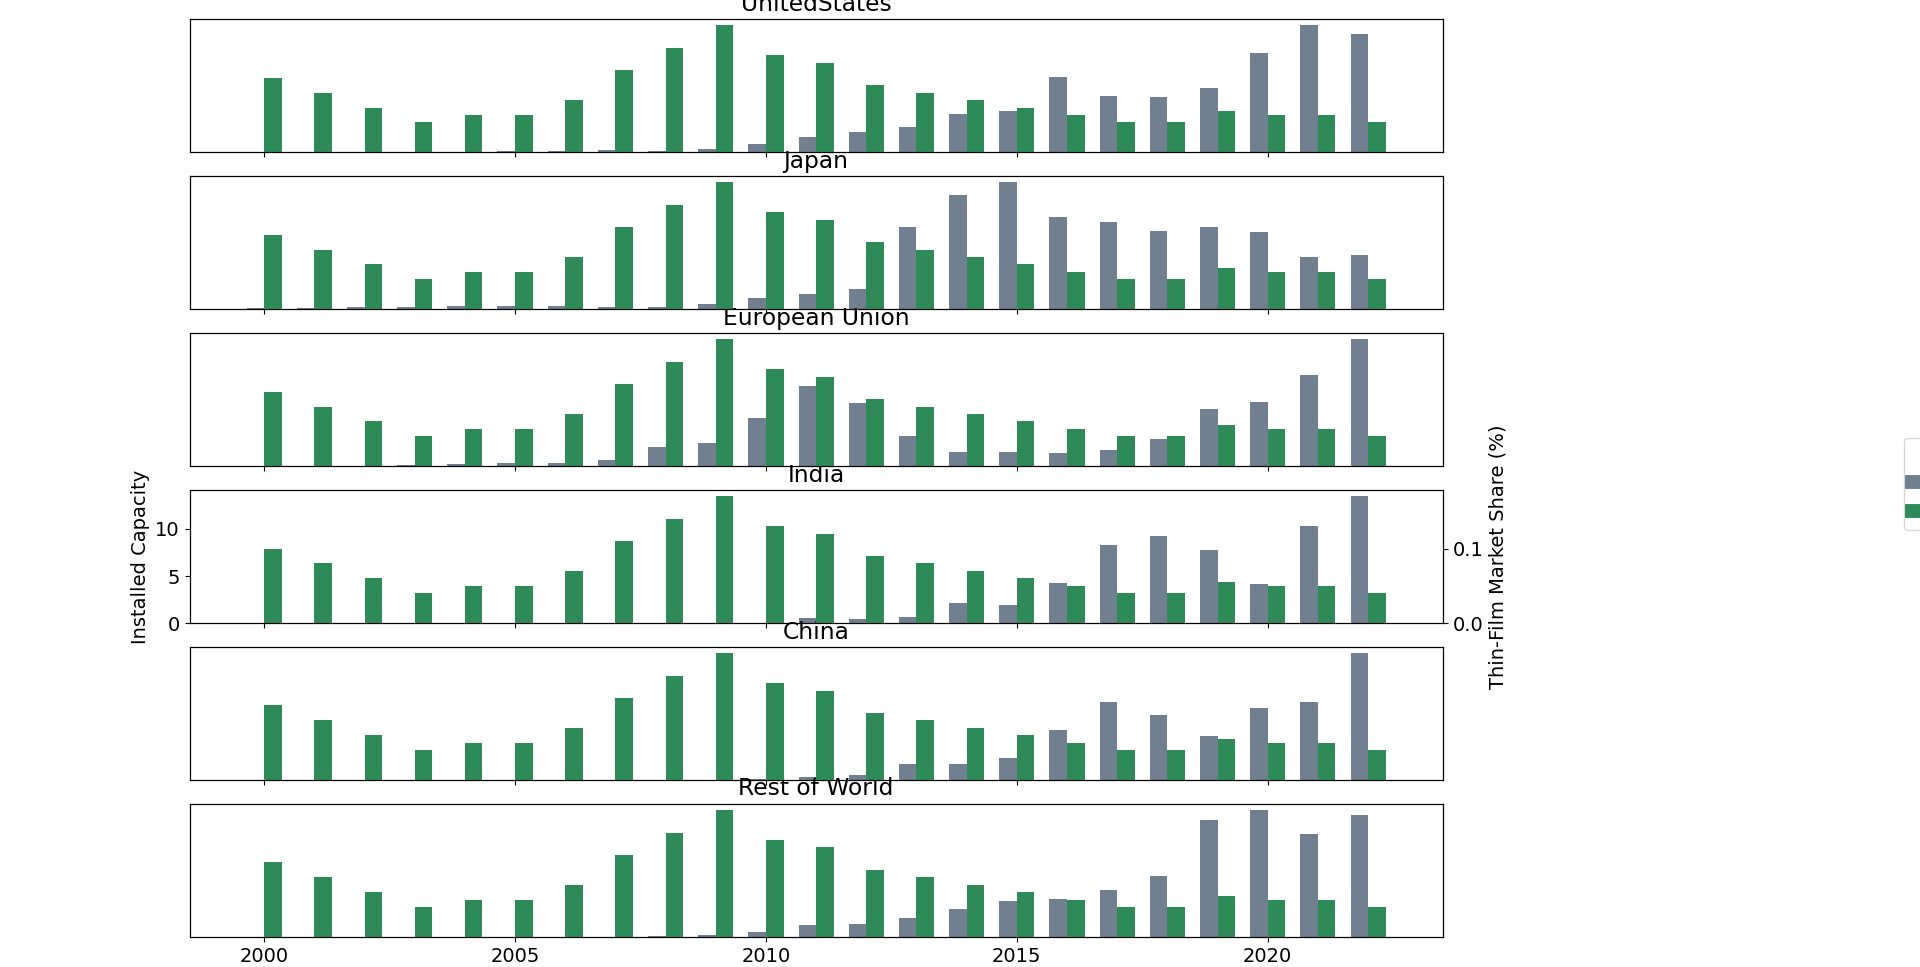
\includegraphics[width=0.5\linewidth]{Figures/Installed Capacity and Thin-film Market Share.png}
%      \caption{Total Capacity Installed and Thin Film Percentage by Country}
%      \label{fig:enter-label}
% \end{figure}

% \begin{figure}
%     \centering
%     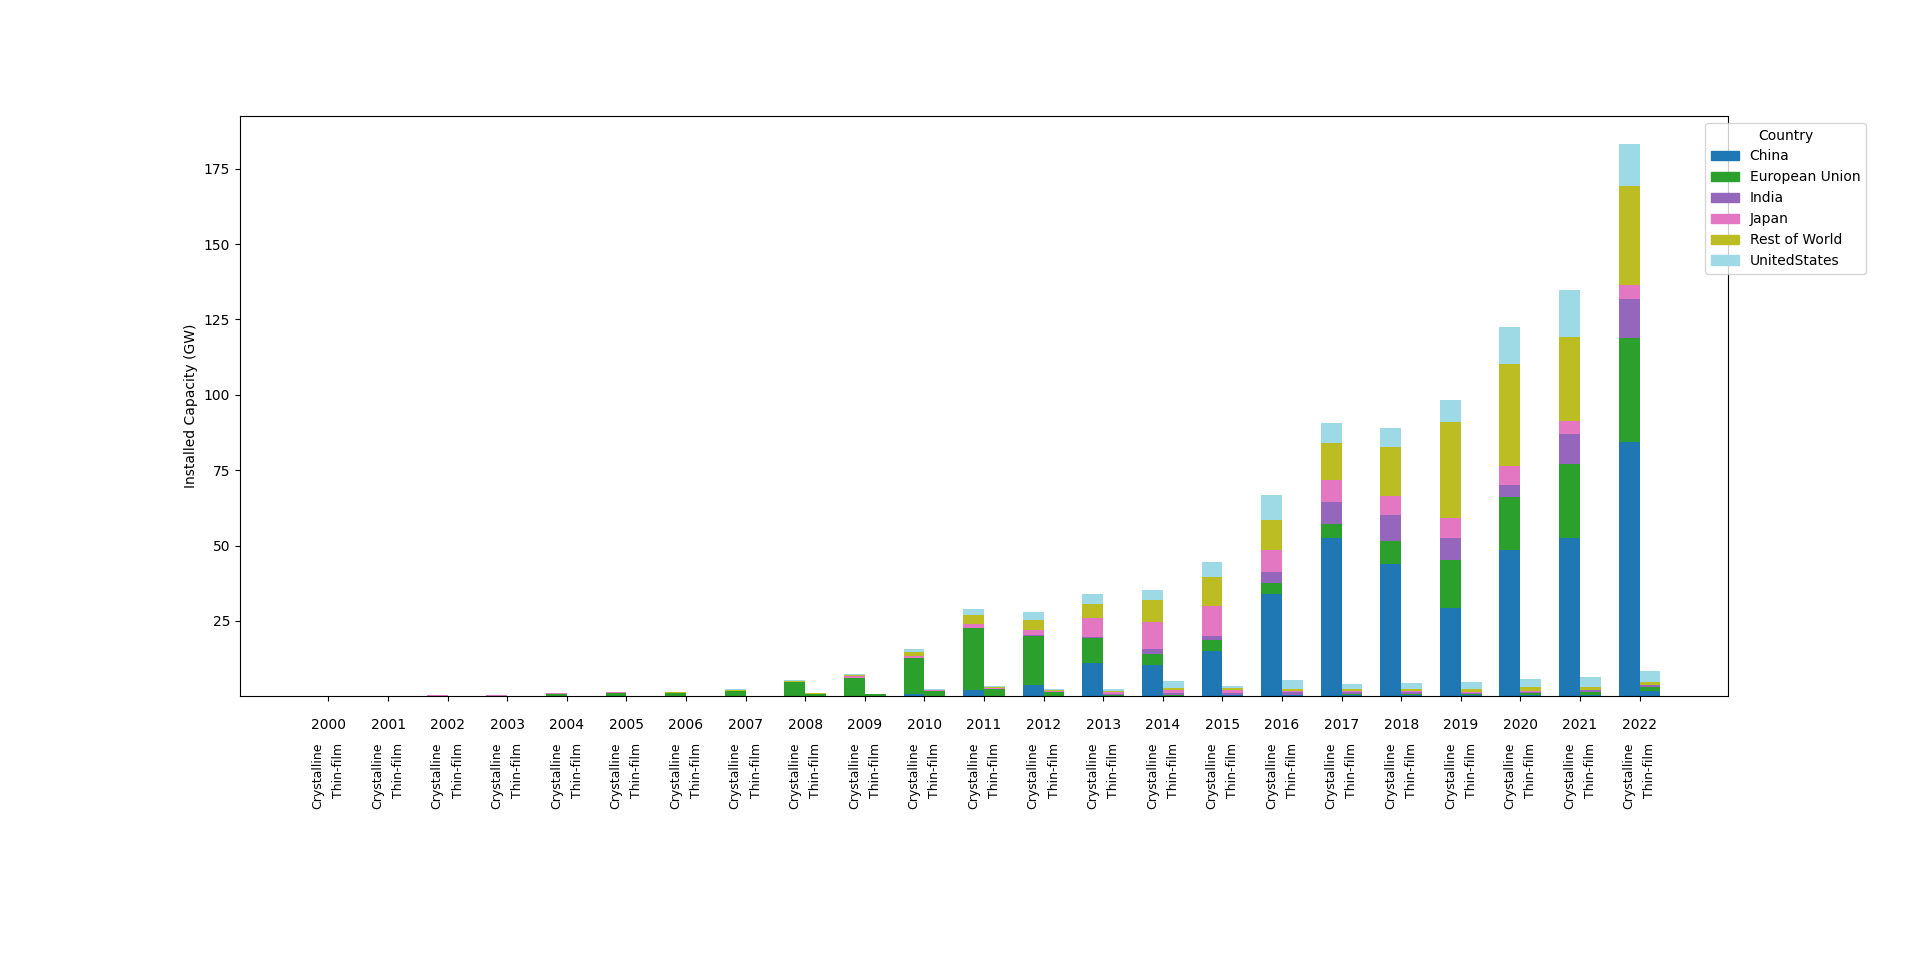
\includegraphics[width=0.5\linewidth]{Figures/Installed Capacity by Country.png}
%     \caption{Total Capacity Installed by Type by Country}
%     \label{fig:enter-label}
% \end{figure}


\begin{figure}[tbh]
\centering
\caption{\label{fig:data_sum_PV_price_region}Solar Panel Price by Region}
\subfloat[c-Si]
{\centering
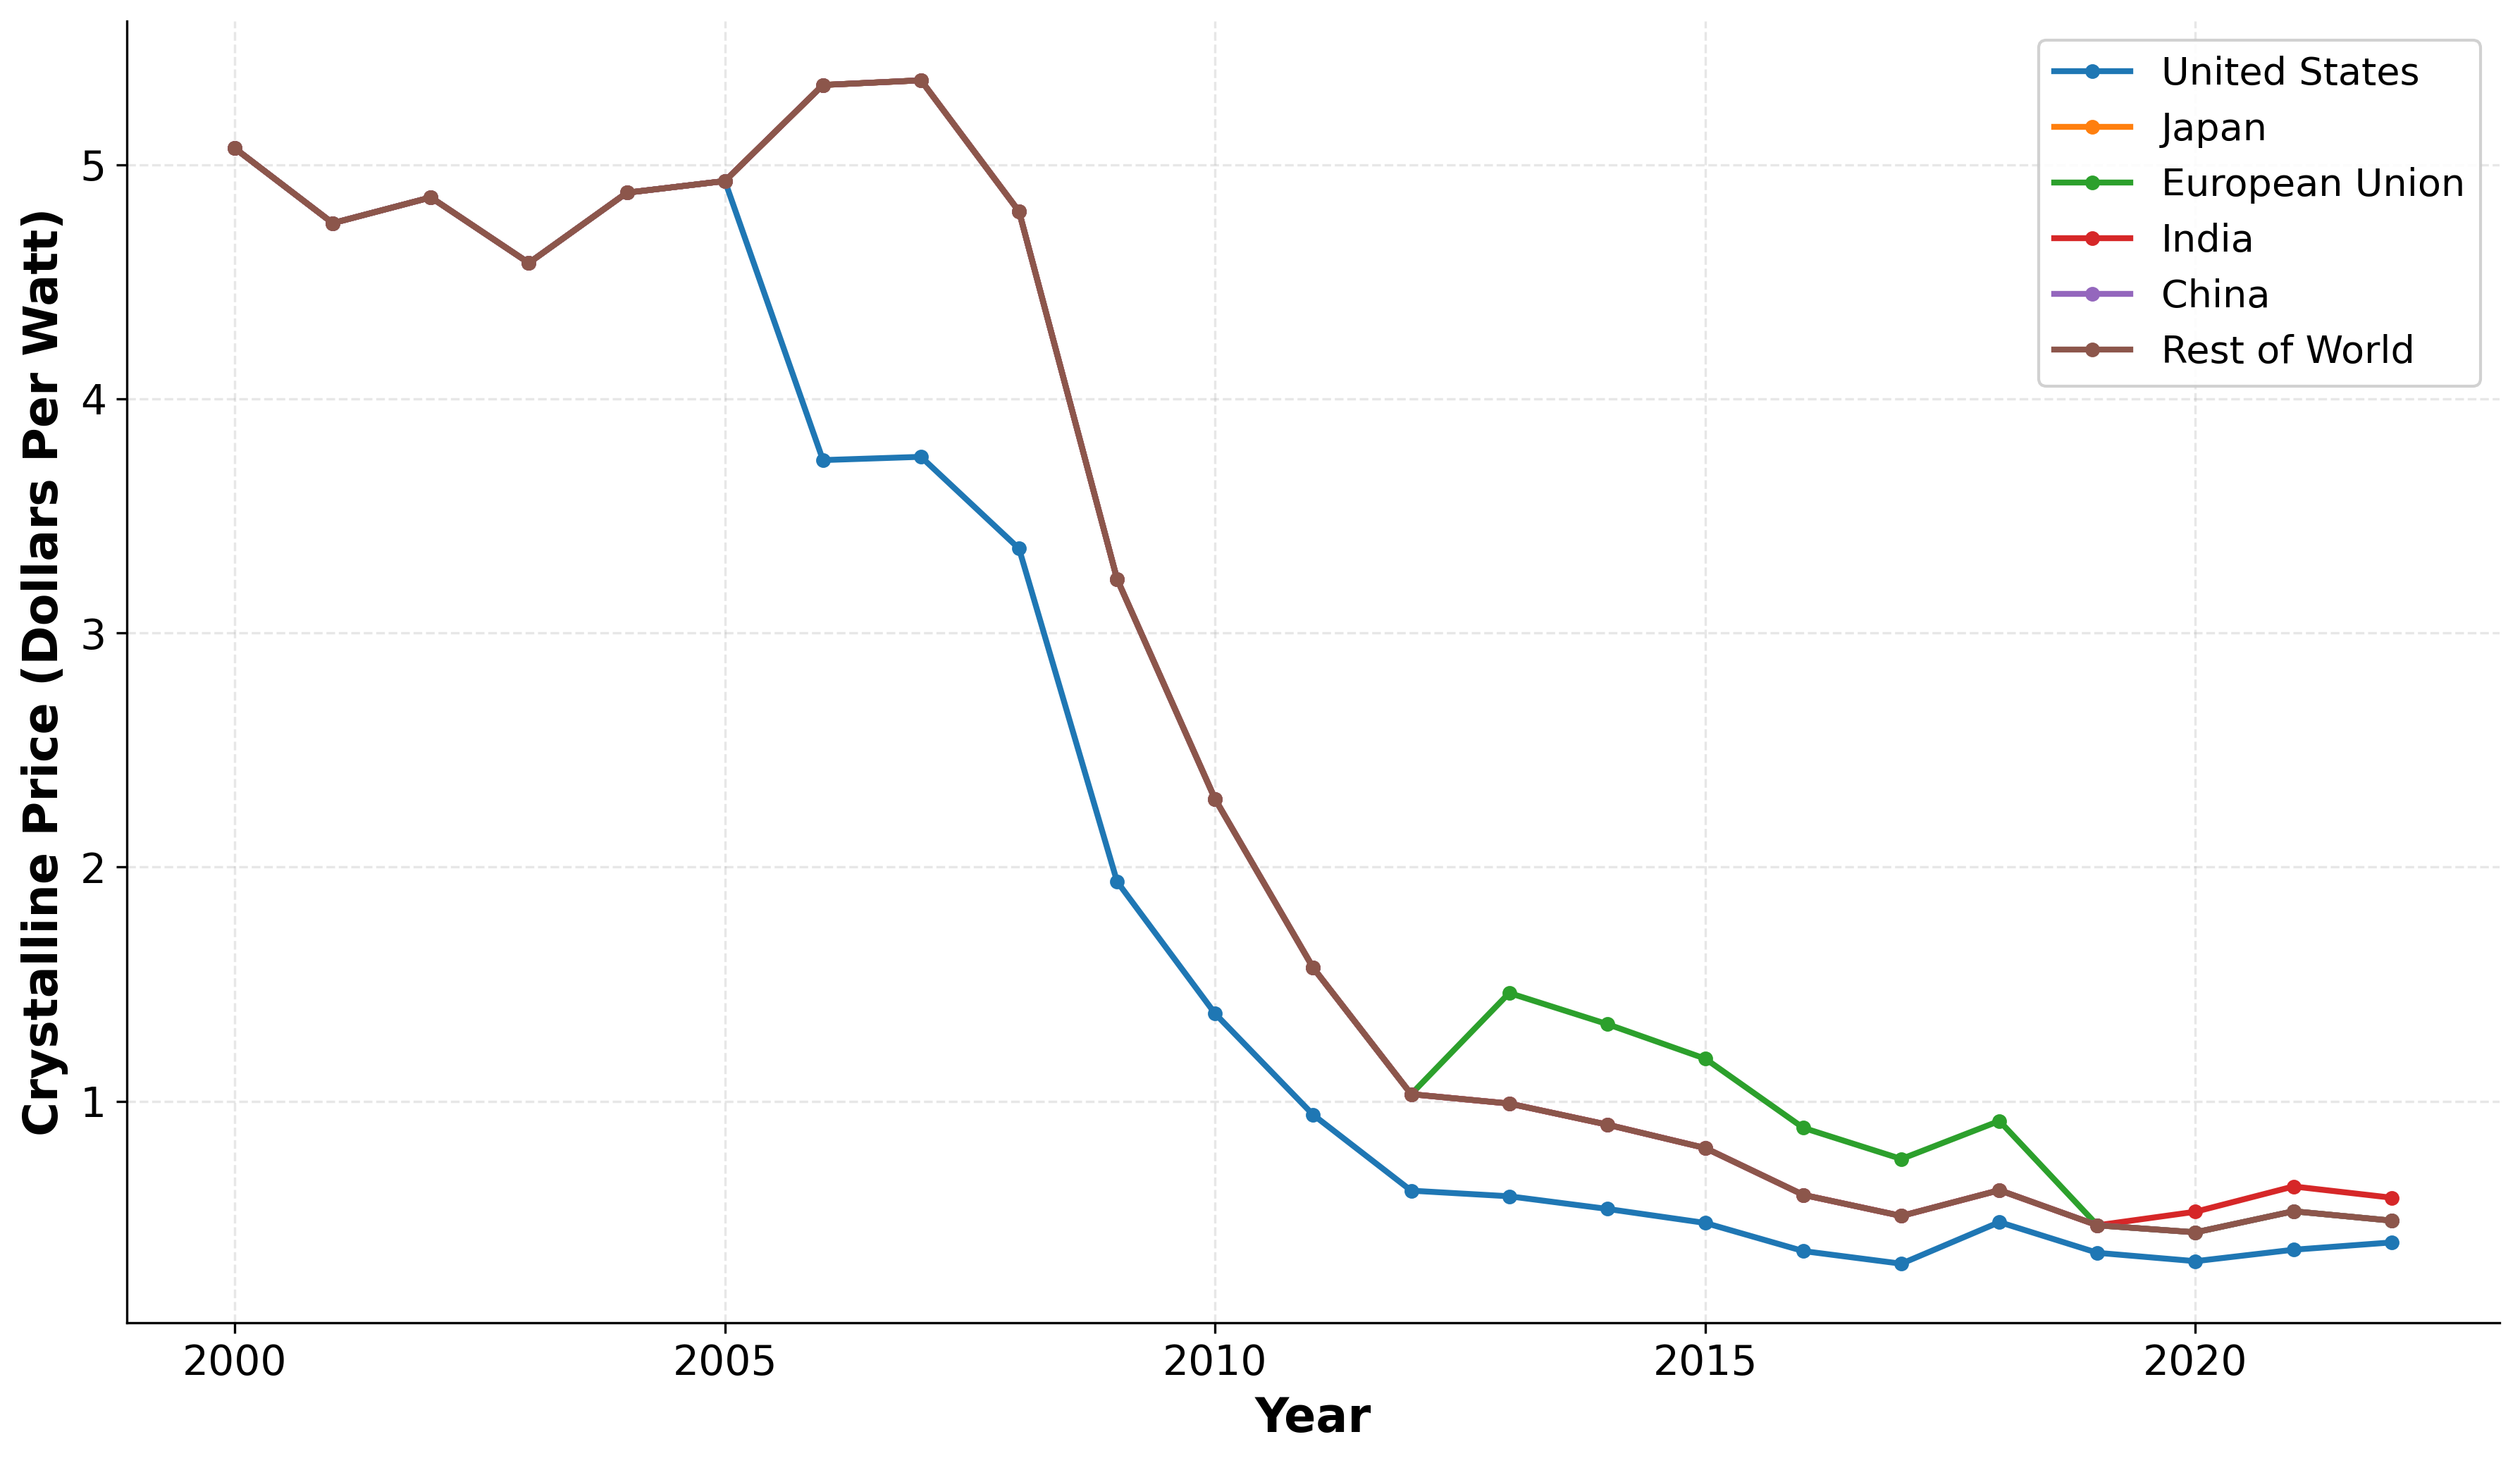
\includegraphics[scale=0.25]{Figures/crystalline_prices_by_country.png}
}
\subfloat[Thin-Film]
{\centering
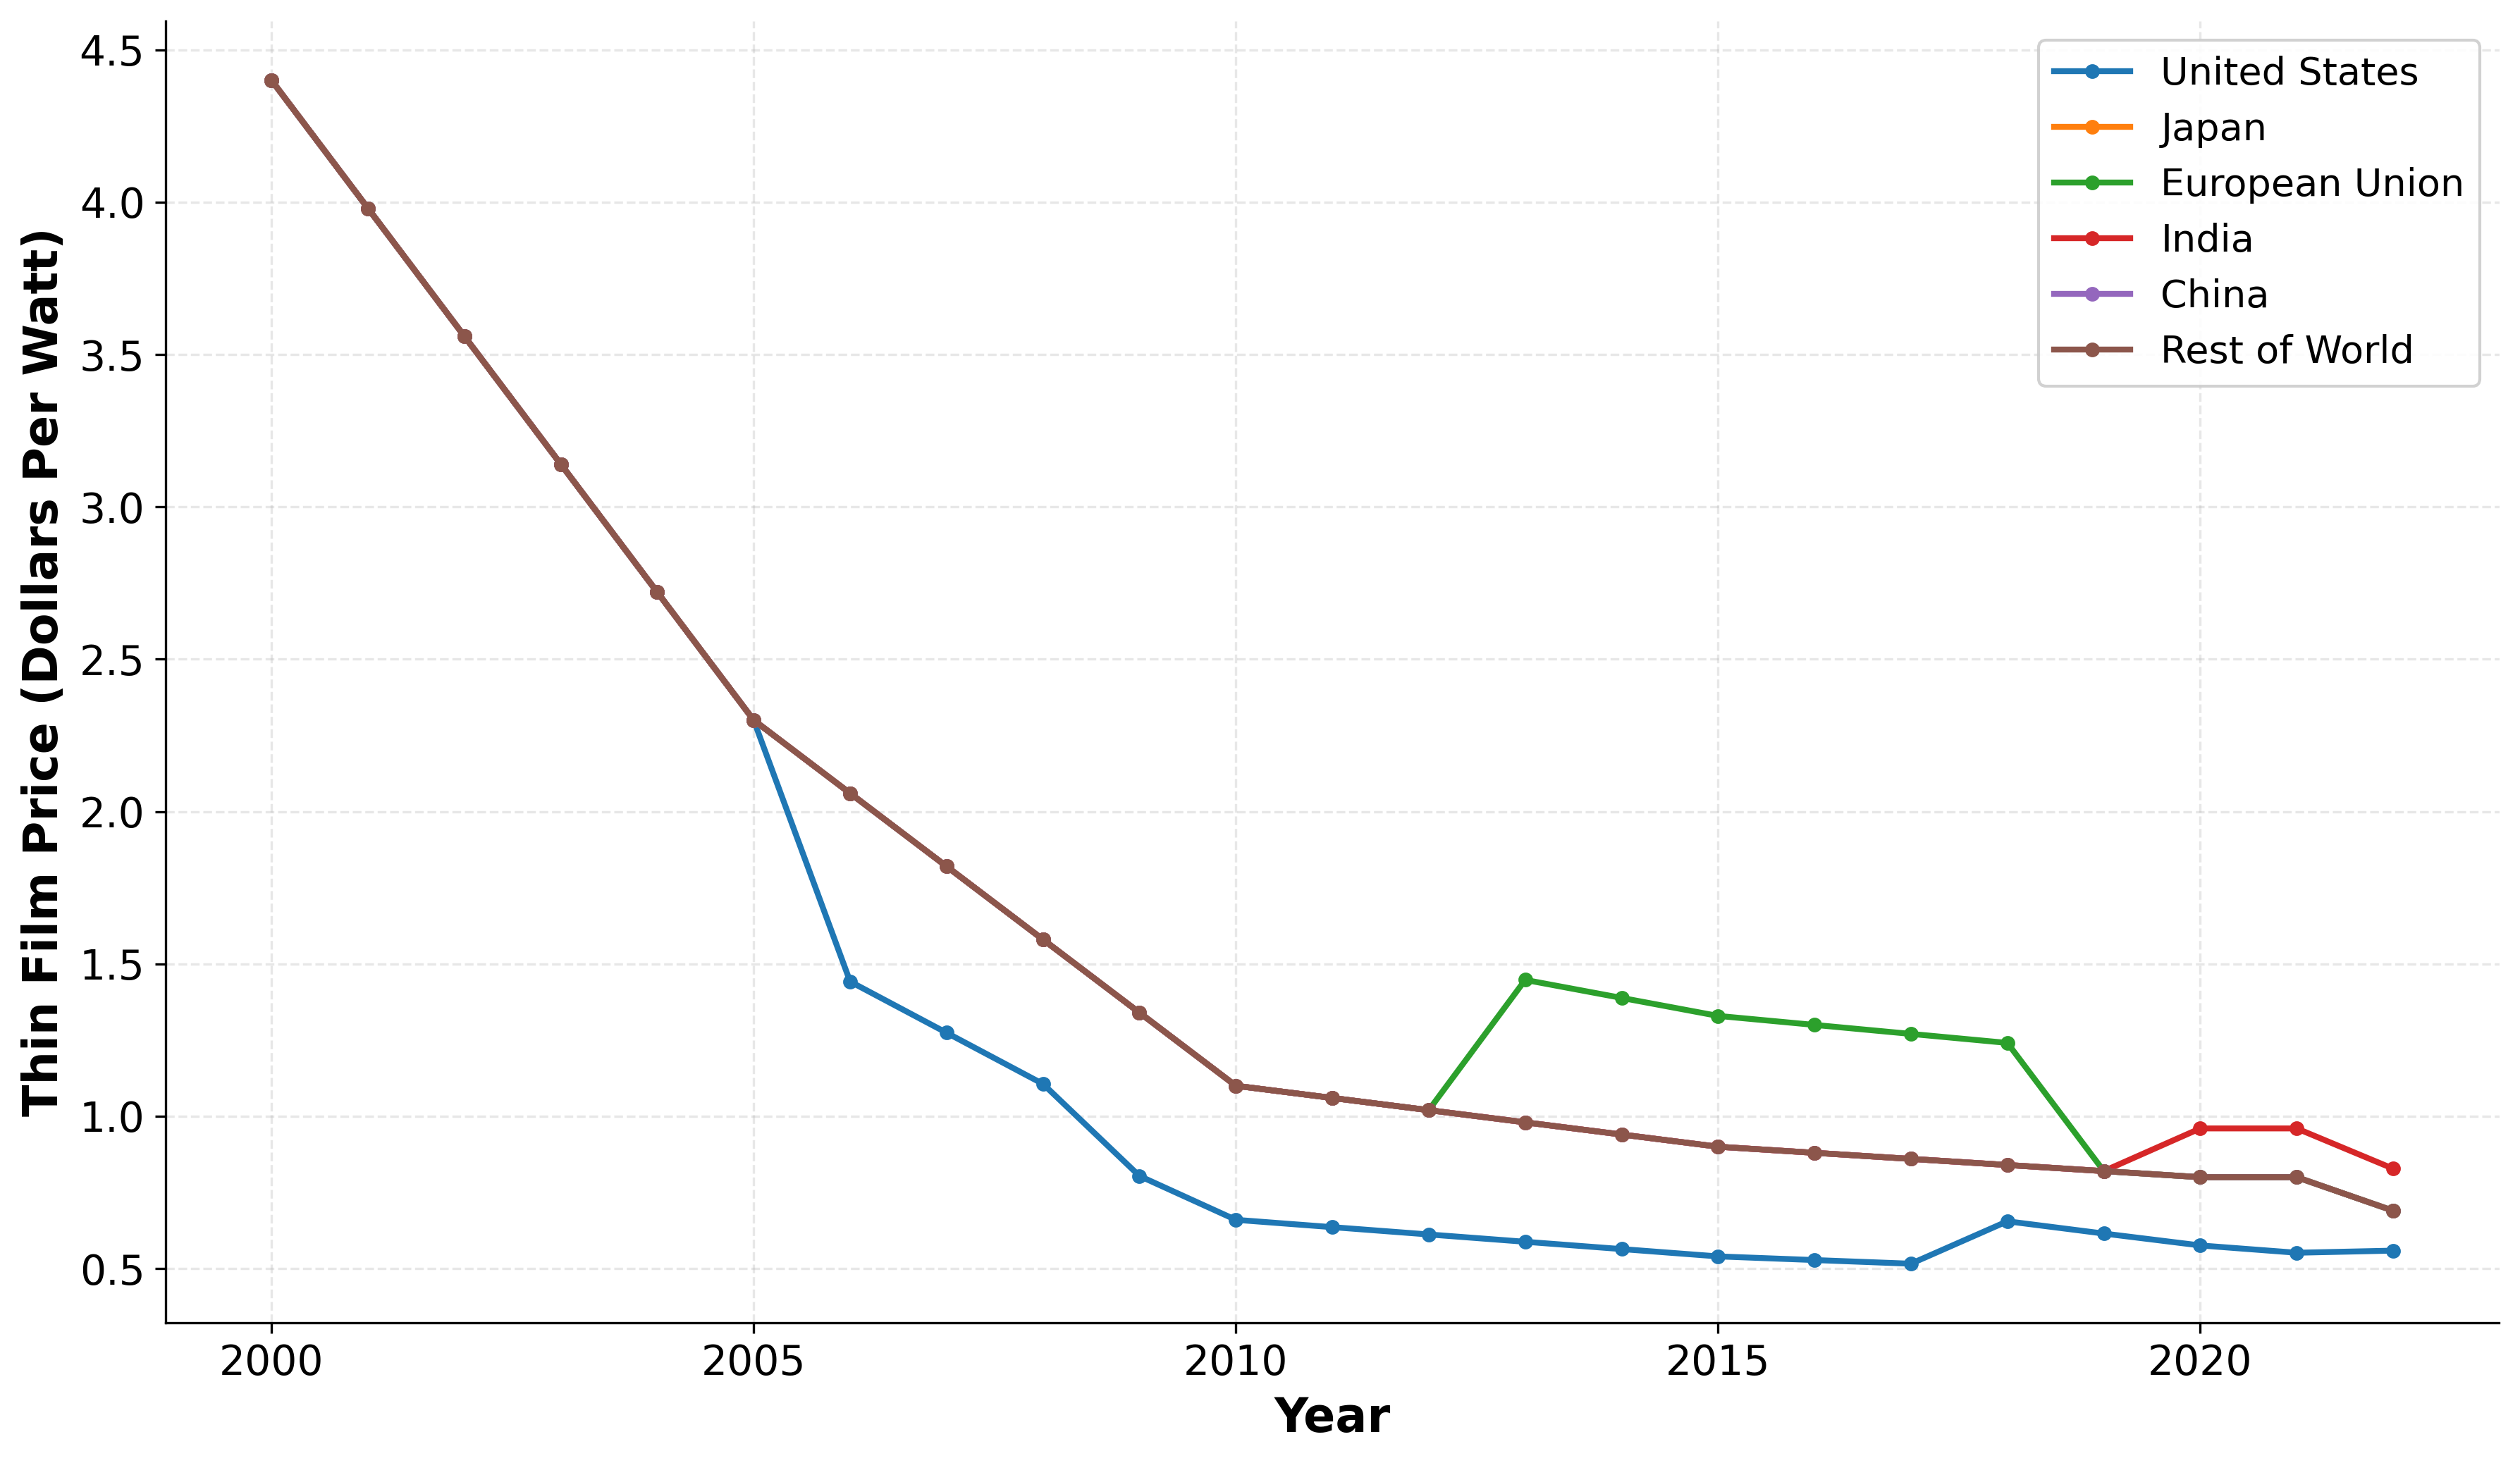
\includegraphics[scale=0.25]{Figures/thinfilm_prices_by_country.png}
}
\end{figure}


\begin{figure}[tbh]
\centering
\caption{\label{fig:data_sum_entry_exit}Entry and Exit of Chinese Solar Panel Manufacturers}
\subfloat[Entry]
{\centering
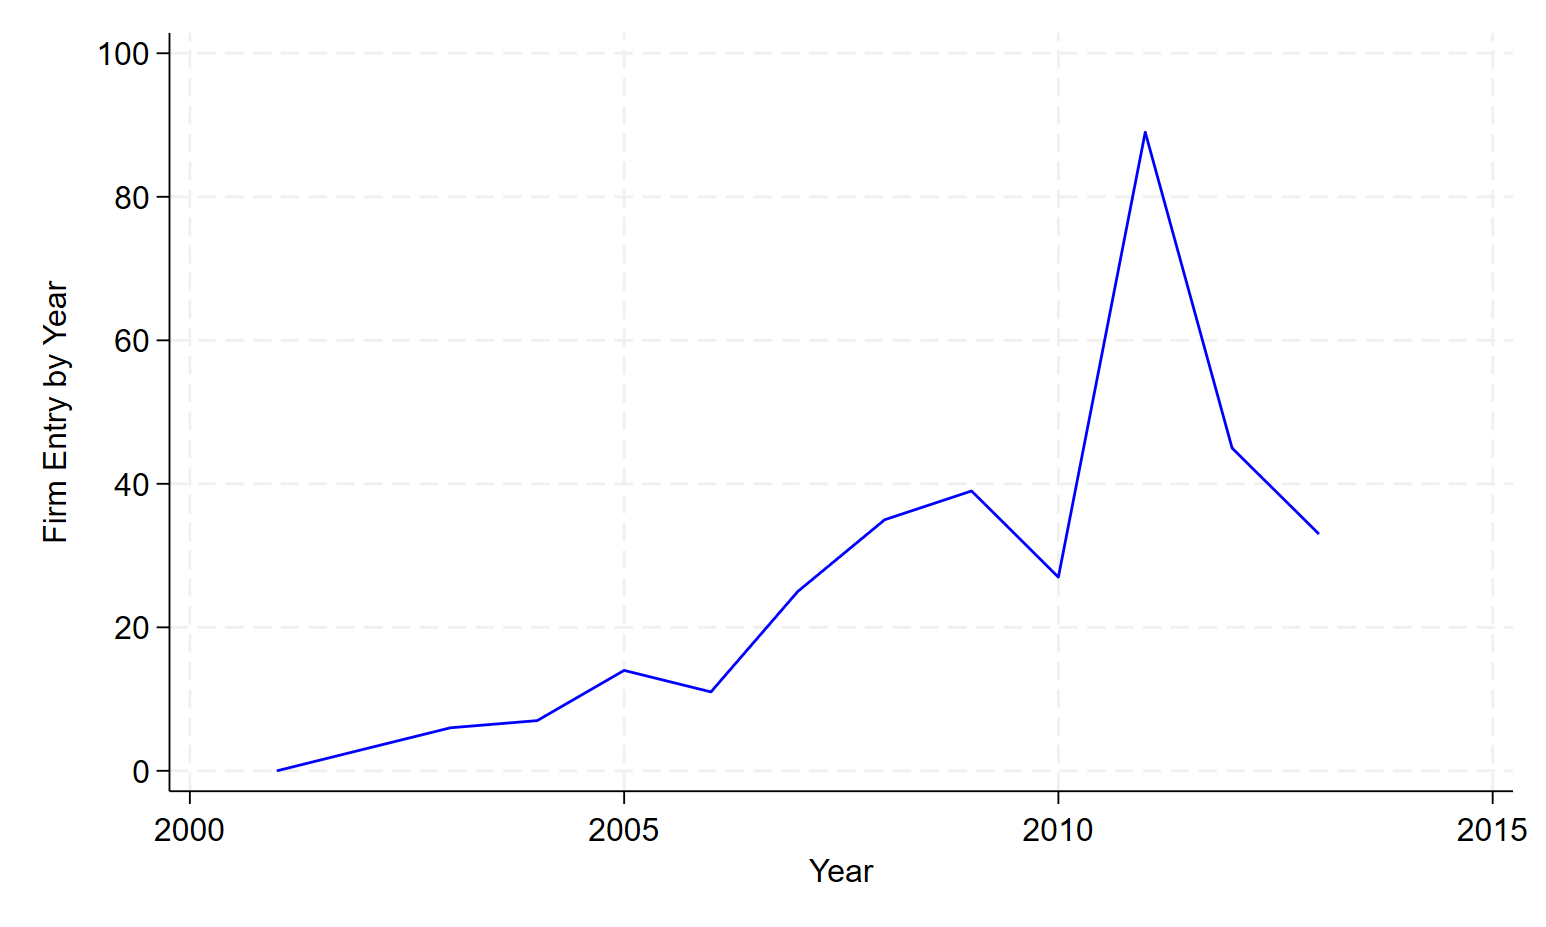
\includegraphics[scale=0.15]{Figures/FirmEntryOverTime.png}
}
\subfloat[Exit]
{\centering
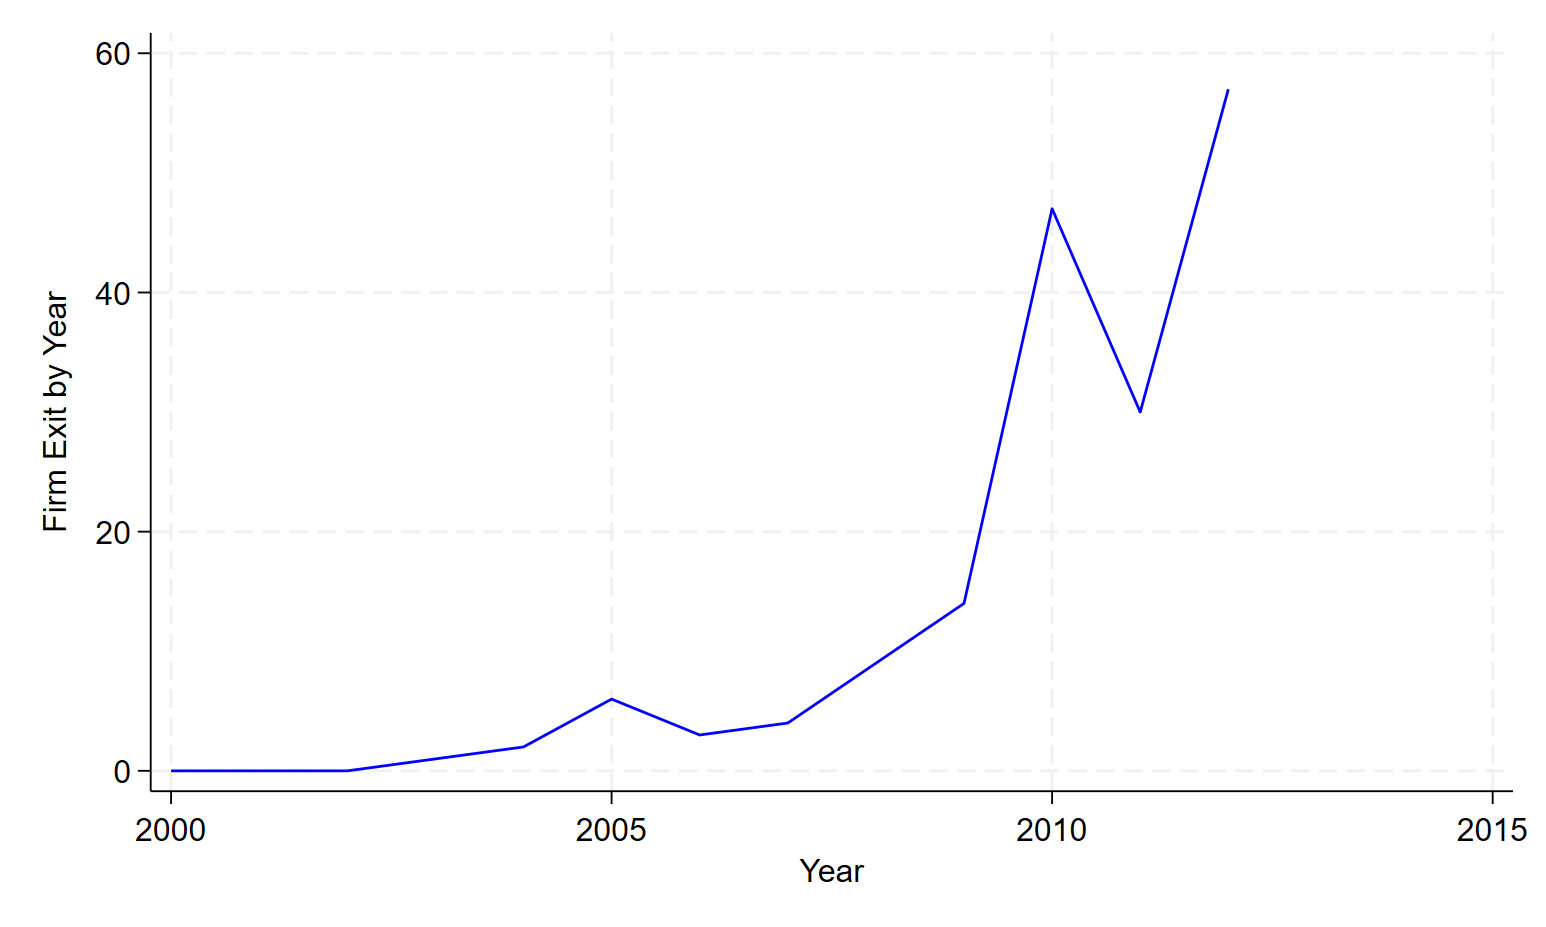
\includegraphics[scale=0.15]{Figures/FirmExitOverTime.png}
}
\end{figure}



\begin{table}[tbh]
\centering
\caption{AR(1) Estimates of State Transition Process}
\label{tab:est_state_transition}
\begin{threeparttable}
\begin{tabularx}{1.00\textwidth}{Xcccccccc}
\toprule
& \multicolumn{2}{c}{Output Price} && \multicolumn{1}{c}{Demand Subsidies} && \multicolumn{3}{c}{Input Price} \\
\cmidrule{2-3} \cmidrule{5-5} \cmidrule{7-9}
 & Poly. & Thin-film && Common && Poly. & Cadmium & Tell. \\
\midrule
$\lambda_0^{pre}$ 
    & 1.596 & -1.570 && 0.021 && 36.799 & 2.272 & 3.238 \\
    & (0.022) & (0.099) && (0.033) && (9.1) & (0.584) & (0.662) \\

$\lambda_0^{post}$ 
    & -1.761 & 7.223 && 0.131 && 6.07 &  &  \\
    & (0.048) & (0.439) && (0.229) && (9.72) &  &  \\

$\lambda_1$  
    & 0.804 &  && -0.053 &&  0.195 & 7.099 & 7.164 \\
    & (0.054) &  && (1.634) && (0.064) & (0.082) & (0.092) \\

\midrule
N 
    & 22 & 22 && 13 && 228 & 31 & 30 \\
$R^2$ 
    & 0.988 & 0.998 && 0.660 && 0.760 & 0.633 & 0.615 \\
AIC 
    & -29.671 & -97.774 &&  &  & 2362.69 & 44.499 & 32.491 \\
\bottomrule
\end{tabularx}
\begin{tablenotes}
    \item Notes: The dependent variable is the price in year $t$. Standard errors in parenthesis. We use different year as the cutoff to define Pre" and Post". The cutoff year is 2008 for the c-Si solar panel and polysilicon price, 2010 for the thin-film solar panel price, 2007 for the Cadmium price, 2011 and for the Tellurium price. The demand subsidies are measured in two ways. \textcolor{blue}{The first one is weighted by a region's share of demand among the all demand, i.e., $\sum_m sub_{mt} * \frac{Q_{mt}}{\sum_{m'}Q_{m't}}$, where $sub_{mt}$ is the demand subsidy in region $m$ and $Q_{mt}$ is the total demand in region $m$. The second one is weighted by the share of a firm's output to a region among this firm's total output, i.e., $\sum_m sub_{mt} * \frac{q_{jmt}}{\sum_{m'}q_{jm't}}$, where $sub_{mt}$ is the demand subsidy in region $m$ and $q_{jmt}$ is firm $j$'s sales to region $m$.} 
    \item Structural break years: Poly solar panel (2009), Thin-film (2010), Input (2019), Cadmium (2007), Tellurium (2001).
\end{tablenotes}
\end{threeparttable}
\end{table}

\end{document}